\documentclass[hidelinks, 11pt]{book}

%- Package imports --------------------------------------------------------------------------------------------------------------------------------------
\usepackage[british, german]{babel}

\usepackage{amsmath} 
\usepackage{amsthm}
\usepackage{amstext}
\usepackage{amssymb}
\usepackage{amsfonts}
\usepackage{breqn}
\usepackage{csquotes}
\usepackage{graphicx} % Necessary to insert images
\usepackage{float} % Image positioning
\usepackage{caption}
\usepackage{enumitem} 
\usepackage{bm} % For the \bm command
\usepackage{setspace} % For line spacing etc.

\usepackage[a4paper, margin=32mm]{geometry}

% \usepackage{setspace}
% \setstretch{1.1}
% \usepackage{parskip}

\usepackage{fancyhdr}  
\fancyhf{} % Clear preset header and footer settings
\renewcommand\headrulewidth{0pt} % Do not display a line between header and content
\fancyfoot[CO, CE]{\thepage} % Display page number at the bottom center of each page
\pagestyle{fancy}

\usepackage[most]{tcolorbox}

\newtcolorbox{abstractframe}[1][]{
    enhanced,
    arc=0pt,
    outer arc=0pt,
    colback=white,
    boxrule=0.8pt,
    #1
}

\usepackage{titlesec} % Customize chapter headings
\titleformat{\chapter}
  {\normalfont\huge\bfseries}
  {\thechapter}{1em}{}

\usepackage{standalone}
  
\usepackage{tikz} % Graph drawing
\usetikzlibrary{graphs, angles, quotes, babel, matrix, decorations.pathreplacing, calc, positioning, backgrounds} 

\newlength\mtxrowsep   \setlength\mtxrowsep{1.5ex}
\newlength\mtxcolsep   \setlength\mtxcolsep{2\arraycolsep}

\tikzset{
  ams/.style={
    baseline=-.7ex,
    % every delimiter/.style={yshift=-1pt},
    every left delimiter/.style={xshift=4pt},
    every right delimiter/.style={xshift=-4pt},
    % every node/.style={inner sep=0pt},
  },
  ams matrix/.style={
    % inner sep=0pt,
    % column sep=\mtxcolsep,
    % row sep=\mtxrowsep,
    matrix of math nodes,
    baseline, 
    left delimiter={[},
    right delimiter={]}, 
    column sep=4pt
  },
  bmatrix/.style={
    ams,
    every matrix/.style={
      ams matrix,
      left delimiter={[},
      right delimiter={]},
    }
  },
}

\newcommand{\mynode} {
    \node[circle, draw=black, fill=black, inner sep=2pt, minimum size=3pt]
}

\tikzstyle{underbrace style}=[decorate,decoration={brace,raise=2mm,amplitude=3pt,mirror},color=gray]
\tikzstyle{underbrace text style}=[font=\tiny, below, pos=.5, yshift=-3mm]


\newcommand*{\boxcolor}{orange}
\makeatletter
\renewcommand{\boxed}[1]{
    \textcolor{\boxcolor}{%
        \tikz[baseline={([yshift=-1ex]current bounding box.center)}] 
        \node [rectangle, minimum width=1ex,rounded corners,draw, fill=red!20] {\normalcolor\m@th$\displaystyle#1$};
    }
}
\makeatother

 
%- Bibliography management ------------------------------------------------------------------------------------------------------------------------------
\usepackage[
    style=alphabetic, 
    backend=biber,
    maxbibnames=9
]{biblatex}

\usepackage{doi} % Displays DOI references as links

\addbibresource{ressources.bib}

\renewbibmacro{in:}{%
  \ifentrytype{article}{}{\printtext{\bibstring{in}\intitlepunct}}}
  
\DeclareFieldFormat[article,periodical]{volume}{\mkbibbold{#1}} % Displays the volume of a journal bold
\DeclareFieldFormat[inproceedings]{number}{\mkbibbold{#1}} % Displays the volume of proceedings bold
\DeclareFieldFormat{url}{Available at\addcolon\space\url{#1}} % Use "Available at: " as prefix for URLs

\DefineBibliographyExtras{british}{\def\finalandcomma{\addcomma}} % Enable Oxford comma

\DeclareSourcemap{ % Always use full journal name
  \maps[datatype=bibtex]{
    \map[overwrite=true]{
      \step[fieldsource=fjournal]
      \step[fieldset=journal, origfieldval]
    }
  }
}


%- Styles -----------------------------------------------------------------------------------------------------------------------------------------------
\theoremstyle{definition}
\newtheorem{definition}{Definition}[section]
\newtheorem{example}[definition]{Example}
\newtheorem{remark}[definition]{Remark}
\newtheorem{question}[definition]{Question}

\theoremstyle{plain}
\newtheorem{theorem}[definition]{Theorem}
\newtheorem{lemma}[definition]{Lemma}
\newtheorem{corollary}[definition]{Corollary}
\newtheorem{proposition}[definition]{Proposition}
\newtheorem{observation}[definition]{Observation}
\newtheorem{claim}{Claim}[definition]
\newtheorem{conjecture}[definition]{Conjecture}

\renewcommand{\labelenumi}{\rm{(\roman{enumi})}}

%- Custom math operators --------------------------------------------------------------------------------------------------------------------------------
\DeclareMathOperator{\tr}{tr}
\DeclareMathOperator{\dist}{dist}
\DeclareMathOperator{\vspan}{span}
\DeclareMathOperator{\rank}{rank}
\DeclareMathOperator*{\argmax}{arg\,max}
\DeclareMathOperator{\supp}{supp}

\newcommand{\N}{\mathbb{N}}
\newcommand{\Z}{\mathbb{Z}}
\newcommand{\Q}{\mathbb{Q}}
\newcommand{\R}{\mathbb{R}}
\newcommand{\C}{\mathbb{C}}

%- Images ------------------------------------------------------------------------------------------------------------------------------------------------
\graphicspath{ {./images/} }


\title{Spectral Graph Theory:\\ Classical Results and Recent Applications in Geometry and Computer Science}
\author{Jakob Edmaier}
\date{8. April 2025}

\def\theexaminer{Prof.~Dr.~Stefan Glock}

\makeatletter
\let\thetitle\@title
\let\theauthor\@author
\let\thedate\@date
\makeatother

\begin{document}

\frontmatter

\selectlanguage{german}
\newgeometry{margin=32mm}
\begin{titlepage}
    \centering
    \onehalfspacing
    
\includegraphics[width=7cm]{uni-logo.png}

    \large
    
    \vspace{1.0cm}
    %\textbf{Lehrstuhl für Diskrete Mathematik}
            
    \vspace{2.5cm}

    \doublespacing
    {\huge{\textbf{\thetitle}}}

    \onehalfspacing
    
    \vspace{2.2cm}

    Bachelorarbeit von

    \vspace{1cm}

    {\LARGE{\textbf{\theauthor}}}
    
    \vspace{0.2cm}

    \vfill

    \begin{tabular}[l]{cc}
        Prüfer: & \theexaminer
    \end{tabular}

    \vspace{2.0cm}
    \thedate
\end{titlepage}

\selectlanguage{british}
\restoregeometry
\cleardoublepage
\chapter*{Abstract}

Spectral graph theory is a subfield of graph theory that studies graphs using the spectral properties of associated matrices, most notably the adjacency matrix.
For an undirected graph, the adjacency matrix is symmetric and therefore has real eigenvalues. 
The set of all eigenvalues, counted with multiplicities, is called the spectrum of the graph.
Interestingly, there are strong connections between the combinatorial properties of a graph and its spectrum, which is why spectral graph theory has found numerous applications over the past decades.

In this thesis, we give an overview of the fundamentals of spectral graph theory. 
We then present some classical results that showcase the connections to the theory of expander graphs and pseudorandomness.
In the second part of the thesis, we discuss two recent applications of spectral graph theory.
The first is a long-standing geometric problem, namely determining the maximum number of equiangular lines with a fixed angle in high dimensions. 
Jiang, Tidor, Yao, Zhang, and Zhao recently solved this problem using tools of spectral graph theory and also gained new insight into the distribution of the eigenvalues of certain graphs: They showed that the second largest eigenvalue of a connected bounded-degree graph has sublinear multiplicity.
As a second application, we analyse Huang's breakthrough proof of the sensitivity conjecture, previously a major open problem in computational complexity theory.

\bigskip
\selectlanguage{german}

\begin{abstractframe}
    \setlength{\parindent}{1em}
    \footnotesize
    \noindent \textbf{Deutsche Zusammenfassung.}
    Die spektrale Graphentheorie untersucht Graphen anhand der Eigenwerte und Eigenvektoren von assoziierten Matrizen, insbesondere der Adjazenzmatrix.
    Für einen ungerichteten Graphen ist die Adjazenzmatrix symmetrisch, und hat daher reelle Eigenwerte. 
    Die Menge aller Eigenwerte, mit Vielfachheiten gezählt, wird als Spektrum des Graphen bezeichnet.
    Interessanterweise bestehen tiefgreifende Zusammenhänge zwischen den kombinatorischen Eigenschaften eines Graphen und seinem Spektrum, weshalb die spektrale Graphentheorie in den letzten Jahrzehnten zahlreiche Anwendungen gefunden hat.
    
    Diese Arbeit gibt zunächst einen Überblick über die Grundlagen der spektralen Graphentheorie. 
    Anschließend präsentieren wir einige klassische Resultate, die u.a. den Zusammenhang mit der Theorie der Expandergraphen illustrieren.
    Im zweiten Teil der Arbeit diskutieren wir zwei aktuelle Anwendungen der spektralen Graphentheorie.
    Als erstes geht es dabei um ein altes geometrisches Problem, nämlich die Bestimmung der maximalen Anzahl von Geraden im hochdimensionalen Raum, die paarweise einen gleichen Winkel einschließen.
    Jiang, Tidor, Yao, Zhang und Zhao haben dieses Problem kürzlich mit Methoden der spektralen Graphentheorie gelöst, und zugleich neue Erkenntnisse über die Verteilung der Eigenwerte bestimmter Graphen gewonnen:
    Die Vielfachheit des zweitgrößten Eigenwerts eines zusammenhängenden Graphen mit beschränktem Maximalgrad ist sublinear.
    Als zweite Anwendung analysieren wir Huang's Beweis der Sensitivity-Vermutung, einem zuvor jahrzehntelang ungelösten Problem der Komplexitätstheorie.
\end{abstractframe}

\selectlanguage{british}

\tableofcontents 

\mainmatter

\chapter{Introduction}

Graph theory is a branch of mathematics concerned with the study of network-like structures called \textit{graphs}.
In this context, a graph consists of a collection of objects (called \textit{vertices}), and any two of these objects may be connected by an \textit{edge}.
Graphs can be used to model all kinds of binary relations. 
For example, the vertices could be a group of people, where two people are connected by an edge whenever they are mutual friends.
In computer science, communication networks are modelled by graphs in which the vertices represent hosts and routers, and the edges represent the communication links between them. 
Navigation systems use graphs to compute the shortest route between two places, and in the natural sciences, graphs can be used, for example, to model chemical structures such as molecules. % (see e.g. \cite{chemicalgraphtheory}).

Leonhard Euler's resolution of the Seven Bridges of Königsberg problem \cite{solutio} is often considered the first mathematical work on graph theory.
Since then, graph theory has evolved into an independent discipline within mathematics.
Over the course of the twentieth century, it has gained particular importance with the rise of computers and the development of theoretical computer science, as many graph-theoretic problems have algorithmic applications and connections to complexity theory.

In addition to combinatorial reasoning, tools from other mathematical disciplines, most notably probability theory, topology, and algebra, have been used to study graphs.
This thesis focuses on spectral graph theory, which investigates the spectral properties of matrices associated with graphs. 
The most natural matrix studied in spectral graph theory is the adjacency matrix. 
For a graph on $n$ vertices, this is an $(n \times n)$ matrix with entries in $\{0, 1\}$, where the entry $(i, j)$ indicates whether there is an edge from the $i$-th vertex to the $j$-th vertex.

In the case of an undirected graph, the adjacency matrix is symmetric. 
Therefore, the spectral theorem from linear algebra implies that all its eigenvalues are real and there exists an orthonormal basis of eigenvectors.
At first glance, it may be surprising that there is a strong interplay between the spectrum and the combinatorial properties of a graph. 
However, upon closer examination, these connections quickly become intuitive, and over the past few decades, a fruitful theoretical framework has been developed.

The simplest of these connections can be illustrated using the example of a $d$-regular graph $G$. 
Suppose that the eigenvalues of the adjacency matrix of $G$ are given by $\lambda_1 \ge \lambda_2 \ge \dots \ge \lambda_n$. 
We will see that:
\begin{itemize}[noitemsep]
    \item The largest eigenvalue satisfies $\lambda_1 = d$.
    \item The graph is connected if and only if $\lambda_1 > \lambda_2$.
    \item The graph is bipartite if and only if $\lambda_1 = -\lambda_n$.
\end{itemize}
Furthermore, a lot of information is provided by the \textit{spectral gap} of $G$, that is, the difference between its largest and second largest eigenvalue.

In addition to revealing interesting structural properties, eigenvalues and eigenvectors of graphs are also useful in their own right:
This can be seen, for example, in Google's PageRank algorithm, which played a key role in the search engine's huge success.
The algorithm ranks the importance of web pages by assigning a numerical weighting to each page.
The idea is that a page which is linked to by more pages should receive a higher weighting, and the higher the weighting of the referencing pages, the higher the weighting of this page (cf. Figure \ref{fig:page-rank}).
The PageRank algorithm achieves this by assigning to each page the corresponding entry of the Perron eigenvector (see Section \ref{section:perron-frobenius}) of an associated matrix of the World Wide Web graph. 
The vertices of the underlying directed graph are web pages $P_1, \dots, P_n$, with an edge from $P_i$ to $P_j$ whenever $P_i$ contains a hyperlink referencing $P_j$.
More details on PageRank can be found in \cite{thelinearalgebrabehindgoogle}.

\begin{figure}[h]
    \centering
    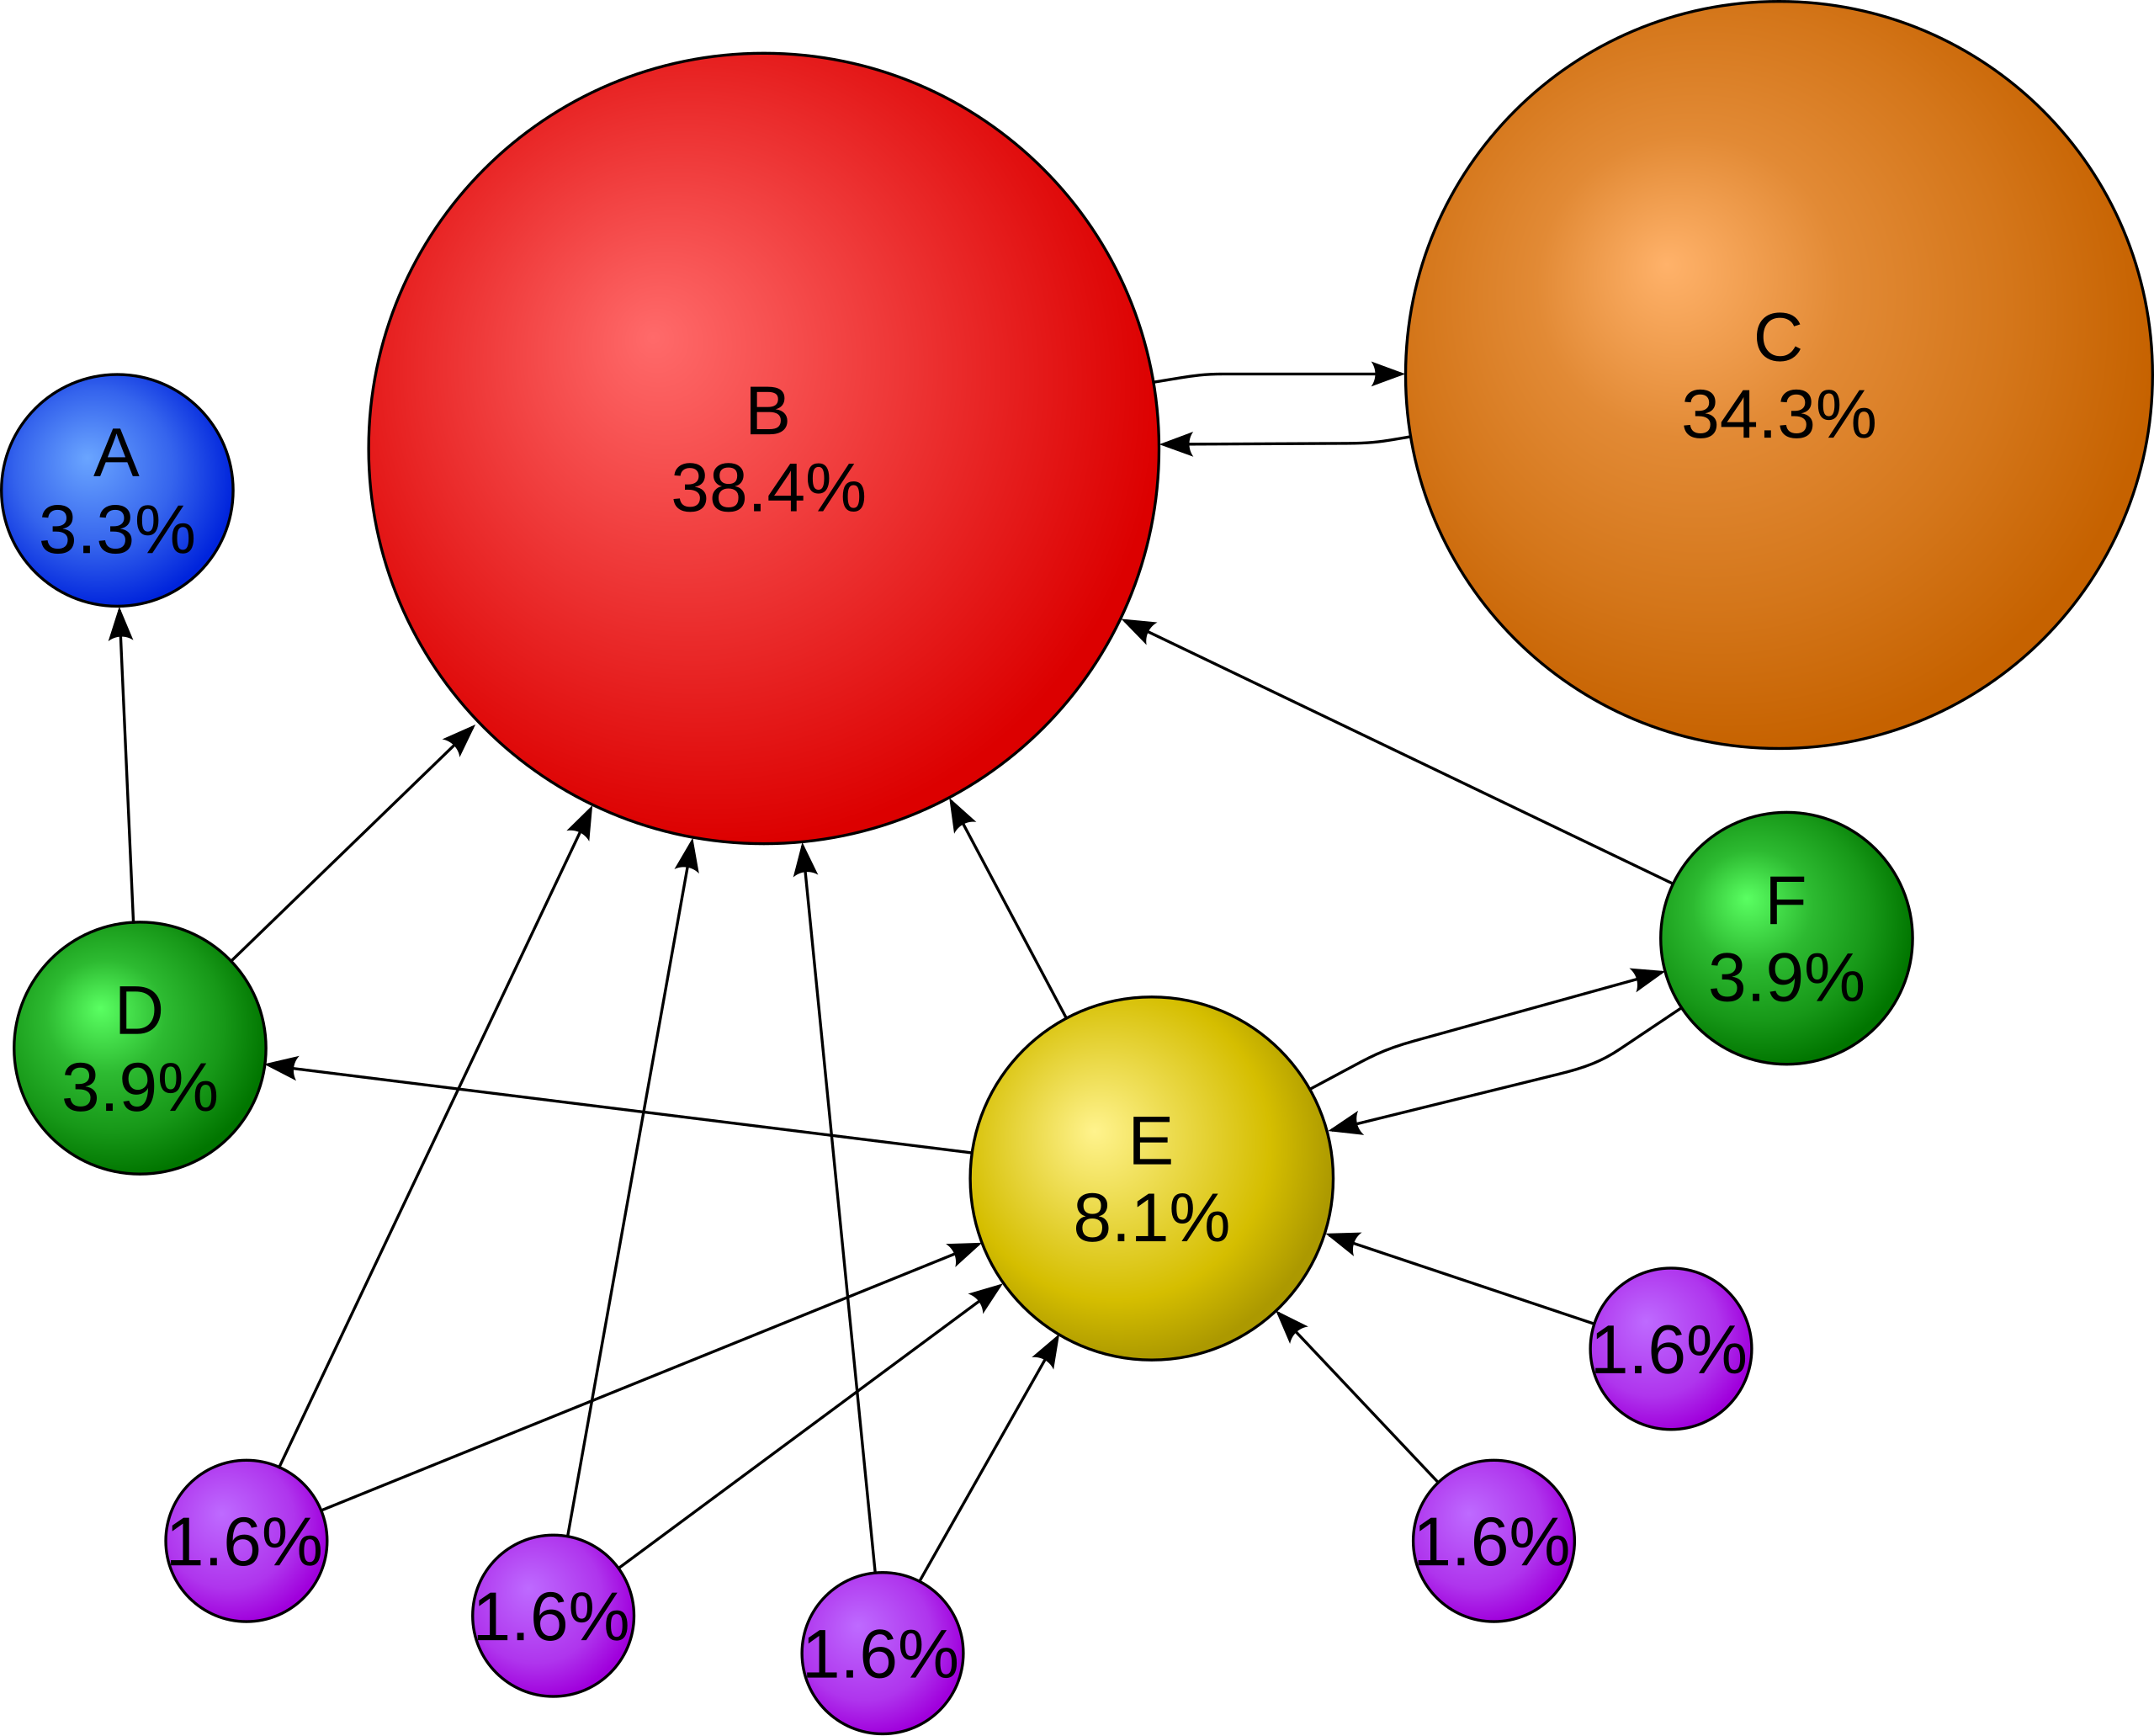
\includegraphics[width=0.6\linewidth]{images/PageRanks-Example.svg.png}
    \caption{The PageRank algorithm applied to a small graph. Taken \mbox{from \cite{wikimedia-pagerank}.}}
    \label{fig:page-rank}
\end{figure}

Furthermore, spectral techniques have been used to give proofs for seemingly purely combinatorial problems such as the Erd\H os--Ko--Rado theorem (see Section \ref{section:hoffman-bound}) or the Sensitivity Conjecture (see Section \ref{section:sensitivity}).

\section{Thesis outline}
The goal of this thesis is twofold.
First, we provide an overview of the foundations of spectral graph theory and present some classical results.
Secondly, we give an in-depth review of two disparate recent research results that showcase the connections of spectral graph theory to geometry and computer science.

In Chapter 2, we start by defining the basic graph-theoretic concepts encountered throughout this thesis, as well as the most prominent matrices that arise in spectral graph theory.
Then, we introduce some useful tools from linear algebra, such as the Perron--Frobenius theorem and the Cauchy interlacing theorem, and apply them to obtain elementary information about the spectrum of the adjacency matrix of a graph.

Chapter 3 presents some classical results from spectral graph theory that relate the combinatorial properties of a graph to its spectrum. 
The first part of this chapter treats the concept of graph expansion and Cheeger's inequality.
Roughly speaking, an expander graph is a (usually sparse) graph with very good connectivity properties, so that one cannot disconnect two large parts of the graph by removing a small number of edges. 
Cheeger's inequality, one of the most important results of spectral graph theory, states that a large spectral gap is qualitatively equivalent to good expansion properties.

In the remainder of this chapter, we cover Hoffman's bound and the Expander mixing lemma.
The former result provides a bound on the independence number in terms of the smallest eigenvalue of a graph, while the latter relates the spectrum of a graph to a particular pseudorandomness property: 
It asserts that the edges of certain regular graphs are "spread out" in the sense that their edge distribution resembles that of a random graph.

Chapters 4 and 5 deal with applications of spectral graph theory to other subfields of mathematics.
In addition to providing insight into specific research topics, both chapters are meant to demonstrate how spectral methods can be used to give surprisingly elegant proofs for problems that have little connection to graph theory at first sight. 
The following two sections provide a first overview of these applications.

Chapter 6 concludes the thesis and hints at possible sources for further reading.

\section{An application in geometry}

In Chapter 4, we discuss the resolution of a long-standing geometric problem concerning equiangular lines. 
Even though the connection to graph theory is far from obvious, the study of equiangular lines is named one of the founding problems of spectral graph theory in the classic textbook Algebraic Graph Theory \cite{godsilroyle} by Godsil and Royle.
For $\alpha \in (0, 1)$, let $N_\alpha (d)$ denote the maximum number of lines with pairwise angle $\arccos \alpha$ in $\R^d$. 
The problem of determining $N_\alpha (d)$ for a fixed $\alpha$ and large dimensions $d$ dates back to 1973, when Lemmens and Seidel \cite{lemmensseidel} introduced the quantity.
In a recent work, Jiang, Tidor, Yao, Zhang, and Zhao \cite{equiangular} solved this problem using tools of spectral graph theory. 
For the case where $\alpha = 1 / (2k - 1)$ for some integer $k \ge 2$ and $d$ is sufficiently large, their main result states that $N_\alpha(d) = \lfloor k (d - 1) / (k - 1) \rfloor$.

A major ingredient in their proof is a novel result in spectral graph theory that gives insight into the distribution of the eigenvalues of a graph:
They showed that the second largest eigenvalue of a connected $n$-vertex graph with bounded maximum degree has multiplicity at most $O(n / \log \log n)$.\footnote{The largest one has multiplicity $1$.}
To the best of our knowledge, this is the first result of this form for general graphs.
Currently, there is still a significant gap between this bound and the best-known lower bound constructions, which achieve a second eigenvalue multiplicity of $n^{1 /2 - o(1)}$.
This led the authors of \cite{equiangular} to ask whether their bound can be improved.
Addressing this question, we end Chapter 4 by establishing stronger bounds for the special case of graph classes with small balanced separators.

\section{An application in computer science}
Chapter 5 presents the recent breakthrough proof of the Sensitivity Conjecture, which has stood as one of the most prominent open problems in theoretical computer science for almost three decades.
The conjecture concerns the relationship between two different complexity measures for Boolean functions, \textit{sensitivity} and \textit{block sensitivity}. 
Posed by Nisan and Szegedy \cite{nisanszegedy} in 1992, the Sensitivity Conjecture states that these complexity measures are polynomially related (and hence equivalent in the sense of complexity theory).
Although numerous researchers had previously worked on the problem, very little progress was made until 2019, when Huang \cite{sensitivity} finally published a proof of the conjecture. 
His work builds upon a reduction due to Gotsman and Linial \cite{gotsmanlinial}, according to which it suffices to show that every induced subgraph of the $n$-dimensional hypercube on more than half of the vertices has maximum degree at \mbox{least $\sqrt{n}$}.
Huang's proof uses techniques from spectral graph theory and is notable for its simplicity and succinctness.

\paragraph{Notation and preliminaries.}
By $\N$ we denote the set of natural numbers starting from $1$; to include 0 we write $\N_0$. 
By $[n]$ we denote the set $\{1, 2, \dots, n\}$. 
Given a set $X$ and $k \le |X|$, we write $\binom{X}{k}$ for the set of all $k$-element subsets of $X$.

The $(n \times n)$-identity matrix is denoted by $I_n$. 
Similarly, we write $J_{m,n}$ for the $(m \times n)$ all-ones matrix, or $J_n$ for a square matrix.
If the size can be inferred from the context, we will usually drop the subscript.

We view $\R^n$ together with the Euclidean norm and scalar product throughout.
That means, for vectors $\bm{x}, \bm{y} \in \R^n$, we write $\langle \bm{x}, \bm{y} \rangle := \bm{x}^T \bm{y}$, and $\| \bm{x} \|\; := \sqrt{\langle \bm{x}, \bm{x} \rangle}$.
Vectors are denoted in bold as $\bm{x}, \bm{y}, \bm{v}, \bm{w}$ etc. to distinguish them from graph vertices $x, y, v, w, \dots$, which are typically named with the same letters.
It may occur that the vertices of a graph are vectors themselves.
In this case, we only use bold notation when we want to emphasise this feature.
The all-ones vector is denoted by $\bm{1}$, the $j$-th unit vector is denoted \mbox{by $\bm{e}_j$}.

All logarithms are taken to base $e$, unless denoted otherwise by a subscript.

The reader is assumed to be familiar with elementary linear algebra, especially concepts such as eigenvalues and orthonormal bases.
Standard results that can be found in most undergraduate textbooks, such as the rank-nullity theorem or the spectral theorem, will be used without further explanation. 
All necessary graph-theoretic notions, on the other hand, will be defined in the thesis.

\chapter{Fundamentals}

\section{Basic concepts of graph theory}
In this section, we formally introduce the basic concepts of graph theory, mostly following the terminology used in \cite{diestel}.

\begin{definition}
    An \textit{(undirected) graph} is a pair $G = (V, E)$, where $V$ is a non-empty finite set and $E \subseteq {\binom{V}{2}}$ is a set of 2-element subsets of $V$.
    The elements of $V$ are the \textit{vertices} of $G$, and the elements of $E$ are its \textit{edges}. 
    
    A vertex $x$ is \textit{incident} with an edge $e$ if $x \in e$. 
    For an edge $e = \{v, w\}$ we usually just write $vw$ (or $wv$). We say that $e$ \textit{joins} the vertices $v$ and $w$, and $v, w$ are its \textit{ends} or \textit{endvertices}. 
    Furthermore, $v, w$ are called \textit{adjacent} or \textit{neighbours}, and we occasionally denote that by $v \sim w$.

    For any graph $G$ we refer to its vertex set as $V(G)$ and to its edge set as $E(G)$. The number of vertices of a graph $G$ is called its \textit{order}, denoted by $|G|\;:= |V(G)|$. The number of edges is denoted by $e(G) := |E(G)|$.
\end{definition}

Unless explicitly stated, all graphs considered in this thesis are undirected. 
For a directed graph $G$, the definition is essentially the same as for undirected graphs except that $E \subseteq V^2$, i.e. edges are given an ordering and loops are allowed. 
An edge $e = (x, y)$ in $G$ is directed \textit{from} $x$ \textit{to} $y$; $x$ is called its \textit{tail}, and $y$ its \textit{head}.


\begin{example}
    Graphs are typically displayed by drawing a dot for every vertex and connecting adjacent vertices by a line.
    For most purposes, the positioning of the dots and the shape of the lines are not considered important. 
    The relevant information is just which vertices are connected by an edge.
    
    \begin{figure}[H]
        \centering
        \begin{tikzpicture}
            % Define the vertices with manual positions
            \mynode (v1) at (0, 0) [below left] {};
            \mynode (v2) at (1.5, 0.25) {};
            \mynode (v3) at (3, 0) {};
            \mynode (v4) at (-0.5, 1) {};
            \mynode (v5) at (3, 1) {};
            \mynode (v6) at (0.5, 2) {};  % This can be outside for clarity
            \mynode (v7) at (2, 2) {};  % This can be outside for clarity
            
            \node at (v1) [below left] {1};
            \node at (v2) [right  = 0.1cm] {2};
            \node at (v3) [below right] {3};
            \node at (v4) [left  = 0.1cm] {4};
            \node at (v5) [right = 0.1cm] {5};
            \node at (v6) [above  = 0.1cm] {6};
            \node at (v7) [above right] {7};
        
            % Draw the edges
            \draw (v6) -- (v5);
            \draw (v1) -- (v2);
            \draw (v2) -- (v7);
            \draw (v7) -- (v1);
            \draw [-] (v1) .. controls (1.5, -0.75) .. (v3); % Curved line
        \end{tikzpicture}
        \captionsetup{justification=centering, margin=2cm}
        \caption{Graph with vertex set $V = \{1, \dots, 7\}$ and edge set $E = \big\{ \{ 1, 2\}, \{ 1, 3\}, \{ 1, 7\}, \{ 2, 7\}, \{ 5, 6\} \big\}$}
        \label{fig:example-graph}
    \end{figure}
\end{example}

The next example introduces special graphs that are frequently used as examples or counterexamples.
\begin{example} \label{ex:special_graphs}
    \begin{enumerate}
        \item[(a)] The graph $K_n$ on $n$ vertices in which all vertices are pairwise adjacent is called the \textit{complete graph} of order $n$.

        \begin{figure}[H]
            \centering
            \begin{tikzpicture}
                % Define the vertices
                \foreach \i in {1, 2, 3, 4, 5} {
                    \mynode (v\i) at ({360/5 * (\i - 1) + 90} : 1.5) {};
                }
            
                % Draw the edges to form the cycle
                \draw (v1) -- (v2);
                \draw (v1) -- (v3);
                \draw (v1) -- (v4);
                \draw (v1) -- (v5);
                \draw (v2) -- (v3);
                \draw (v2) -- (v4);
                \draw (v2) -- (v5);
                \draw (v3) -- (v4);
                \draw (v3) -- (v5);
                \draw (v4) -- (v5);
                \draw (v5) -- (v1);
            \end{tikzpicture}
    
            \caption{The complete graph $K_5$}
            \label{fig:complete-graph}
        \end{figure}

        \item[(b)] The \textit{path} $P_n$ of length $n$ is a graph of the form 
        \begin{align*}
            V(P_n) = \{x_0, x_1, \dots, x_n\}, && E(P_n) = \{x_0 x_1,\, x_1 x_2,\, \dots,\, x_{n - 1} x_n\} .
        \end{align*}
        The vertices $x_0$ and $x_n$ are called the \textit{ends} of the path, $x_1, \dots, x_{n - 1}$ its \textit{inner vertices}. 

        \item[(c)] The \textit{cycle} $C_n$ of length $n$ is a graph of the form
        \begin{align*}
            V(C_n) = \{x_1, x_2, \dots, x_n\}, && E(C_n) = \{x_1 x_2,\, x_2 x_3,\, \dots,\, x_{n - 1} x_n,\, x_n x_1\} .
        \end{align*}

        \item[(d)] The $n$-dimensional \textit{hypercube} $Q_n$ has the vertex set $V(Q_n) = \{ 0, 1 \}^n$, with two vertices being neighbours if they differ in exactly one coordinate.
        
    \end{enumerate}
\end{example}

Two graphs are defined as equal if and only if they have the same vertex set and the same edge set. 
While this is a completely natural and reasonable definition, it is also quite restrictive: of course, renaming vertices does not really change the internal structure of a graph. 
This motivates the following definition:

\begin{definition}
    Let $G, G'$ be two graphs. An \textit{isomorphism} (from $G$ to $G'$) is a bijection $\varphi: V(G) \rightarrow V(G')$ satisfying 
    \begin{equation*}
        \varphi(x) \varphi(y) \in E(G') \ \Longleftrightarrow  \ xy \in E(G)
    \end{equation*}
    for all $x, y \in V(G)$. If such an isomorphism exists, $G$ and $G'$ are \textit{isomorphic}, and we write $G \cong G'$.
\end{definition}

Graph isomorphism defines an equivalence relation on the class of all graphs. 
Informally speaking, if two graphs are isomorphic, they are equal "up to labelling". 
Most of the time, we are interested in properties of graphs that do not depend on the names of the vertices and do not distinguish between isomorphic graphs.
Therefore, it is justified, for example, to speak of \textit{the} complete graph on $n$ vertices.

\begin{definition}
    Let $G$ be a graph. 
    A graph $H$ is a \textit{subgraph} of $G$ (and $G$ a \textit{supergraph}), denoted $H \subseteq G$, if $V(H) \subseteq V(G)$ and $E(H) \subseteq E(G)$. 
    If $V(H) = V(G)$, $H$ is called \textit{spanning}.
    A subgraph $H$ of $G$ is called \textit{induced} if
    \begin{equation*}
        E(H) = \{ e \in E(G) : e \subseteq V(H) \}.
    \end{equation*}
    An induced subgraph is thus determined by its vertex set, and for any $U \subseteq V(G)$ we denote by $G[U]$ the induced subgraph of $G$ with vertex set $U$. 

    Furthermore, for $U \subseteq V(G)$ we denote by $G - U$ the subgraph induced by $V(G) \setminus U$, i.e. the graph obtained from $G$ by deleting the vertices from $U$ (and all edges incident with $U$). 
    Similarly, if $F$ is a subset of $E(G)$, we denote by $G - F$ the subgraph of $G$ with vertex set $V(G)$ and edge set $E(G) \setminus F$. 
    If $U = \{ v \}$ or $F = \{ e \}$ we simply write $G - v$, respectively $G - e$.
    If $H$ is a subgraph of $G$, we usually write $G \setminus H$ rather than $G - V(H)$.
    Given two non-adjacent vertices $x, y \in V(G)$, $G + xy$ denotes the graph that is obtained from $G$ by adding an edge between $x$ and $y$.
\end{definition}

\begin{definition}
    Let $G$ be a graph.
    A \textit{walk} $W$ (of length $l$) is a sequence $x_0, x_1, \dots, x_l$ of vertices in $G$ such that $x_{i - 1} x_i \in E(G)$ for all $i \in [l]$.
    We refer to such a walk as an $x_0,x_l$-walk.
    If $x_0 = x_l$, the walk is \textit{closed}.

    The walk $W$ is a \textit{path} if all its vertices are pairwise distinct. We say that $x_0, x_l$ are its \textit{endvertices}, and $x_0, x_l$ are \textit{linked} by $W$.
    
    If additionally $l \ge 2$ and $x_l x_0$ is an edge in $G$, then the sequence $x_0, x_1, \dots, x_l, x_0$ is called a \textit{cycle} (of length $l + 1$).
\end{definition}

\begin{definition}
    A graph $G$ is called \textit{bipartite} if there is a partition $V(G) = A \cup B$ of the vertices such that any edge has one endvertex in $A$ and the other in $B$.
\end{definition}

Bipartite graphs are exactly those graphs that do not contain a cycle of odd length (see \cite[Theorem I.4]{bollobas}).

\begin{example}
    The \textit{complete bipartite graph} $K_{m,n}$ is a bipartite graph with partition $V(K_{m, n}) = A \cup B$, $|A|\;=m, |B|\;=n$ where any vertex of $A$ is adjacent to any in $B$.
    That means
    \begin{equation*}
        E(K_{m,n}) = \{ ab : a \in A, b \in B \}.
    \end{equation*}
\end{example}

\begin{definition}
    Let $G$ be a graph. Given vertices $x$ and $y$, their distance $\dist_G (x, y)$ is the length of a shortest $x,y$-path in $G$.
    If no such path exists, then $\dist_G (x, y) := \infty$.

    A graph $G$ is \textit{connected} if any two vertices $x, v \in V(G)$ are linked by an $x,y$-path \mbox{in $G$}.
    A maximal connected subgraph of $G$ is called a \textit{(connected) component}. 
    If a graph $G$ has components $C_1, \dots, C_s$, we also say that $G$ is the disjoint union of its components and write $G = C_1 + \dots + C_s$.
\end{definition}

\begin{definition}
    A connected graph $G$ without any cycles is called a \textit{tree}. 
    A \textit{forest} is a graph whose components are trees.
\end{definition}

\begin{proposition}
        Let $G$ be a graph. The following are equivalent: 
    \begin{enumerate}
        \item $G$ is a tree.
        \item $G$ is a minimal connected graph, i.e., $G$ is connected, but $G - xy$ is disconnected for every edge $xy \in E(G)$. 
        \item $G$ is a maximal acyclic graph, i.e., $G$ does not contain any cycles, but for any two nonadjacent vertices $x, y \in V(G)$, $G + xy$ does contain a cycle.
        \item For any two vertices $x, y \in V(G)$, there is a unique $x, y$-path in $G$.
    \end{enumerate}
\end{proposition}

\begin{proof}
    See \cite[Theorems I.5 and I.6]{bollobas}.
\end{proof}

\begin{corollary}
    Every connected graph contains a spanning tree (i.e. a spanning subgraph that is a tree).
\end{corollary}

% \begin{proof}
%     Every minimal connected spanning subgraph of $G$ is a spanning tree.
% \end{proof}

\begin{definition}
    Let $G$ be a graph. 
    For any vertex $v$, the set of neighbours of $v$ is denoted by $N(v) = N_G(v)$.
    Similarly, for any subset $A \subseteq V(G)$, $N_G(A) := \bigcup_{v \in A} N_G(v)$ denotes the neighbourhood of $A$ in $G$.
        
    The \textit{degree} of a vertex $v$ is defined as \mbox{$d(v) = d_G(v) := |N_G(v)|$}, or equivalently as the number of edges incident with $v$.
    A vertex of degree $0$ is \textit{isolated}.

    The \textit{minimum degree} of a vertex in $G$ is denoted by $\delta(G)$,
    the \textit{maximum degree} \mbox{as $\Delta(G)$}.
    The \textit{average degree} of $G$ is defined as 
    \begin{equation*}
        \bar{d} (G) := \frac{1}{|V(G)|} \sum \limits_{v \in V(G)} d_G (v).
    \end{equation*}
    Clearly, $\delta (G) \le \bar{d} (G) \le \Delta (G)$. 
    A graph in which every vertex has degree $d$ is called $d$-\textit{regular}.    
\end{definition}

The next proposition relates the number of edges with the vertex degrees.
\begin{proposition}
    For every graph $G$, 
    \begin{equation*}
        2 e(G) = \sum_{v \in V(G)} d_G(v).
    \end{equation*}
\end{proposition}

\begin{proof}
    The right-hand side counts every edge twice, namely for both of its endvertices.
\end{proof}

Besides the subgraph relation, the minor relation is another important structural containment relation between two graphs.
\begin{definition}
    Let $G, H$ be graphs. The graph $H$ is a \textit{minor} of $G$ if for each vertex $x \in V(H)$ there exists a subset $V_x \subseteq V(G)$ such that the following holds:
    \begin{enumerate}
        \item $V_x \cap V_y = \emptyset$ for distinct $x, y \in V(H)$.
        \item $G[V_x]$ is connected for any $x \in V(H)$.
        \item For each edge $xy$ in $H$ there exists an edge in $G$ joining $V_x$ and $V_y$.
    \end{enumerate}
    The sets $V_x$ are called \textit{branch sets}.
\end{definition}

The minor relation defines a partial ordering on the class of all (finite) graphs. 
Observe that a subgraph $H$ of a graph $G$ is also its minor:
In this case, the branch sets can simply be chosen as $V_x = \{x\}$ for each $x \in V(H)$.
Figure \ref{fig:example-minor} illustrates the above definition.

\begin{figure}[H]
    \centering
    \begin{tikzpicture}

        % Draw the shapes with a light grey background
        \filldraw[fill=gray!30, draw=black, dashed] (0.25, 0.25) circle [radius=0.6];
        \filldraw[fill=gray!30, draw=black, dashed] (3, 0.25) ellipse [x radius=0.4, y radius=0.6];
        \filldraw[fill=gray!30, draw=black, dashed] (0.2, 2.8) circle [radius=0.6];
        \filldraw[fill=gray!30, draw=black, dashed] (3, 3) circle [radius=0.3];

        
        % Define the vertices with manual positions
        \mynode (v1) at (0, 0) {};
        \mynode (v2) at (0, 0.5) {};
        \mynode (v3) at (0.5, 0.5) {};
        \mynode (v4) at (0.5, 0) {};
        \mynode (v5) at (3, 0) {};
        \mynode (v6) at (3, 0.5) {};
        \mynode (v7) at (3, 3) {};
        \mynode (v8) at (4, 3) {};
        \mynode (v9) at (0, 2.5) {};
        \mynode (v10) at (0, 3) {};
        \mynode (v11) at (0.5, 3) {};

        \mynode (v12) at (-1.5, 1.5) {};
    
        % Draw the edges
        \draw (v1) -- (v2);
        \draw (v2) -- (v3);
        \draw (v3) -- (v4);
        \draw (v4) -- (v1);
        \draw[very thick] (v3) -- (v7);
        \draw[very thick] (v4) -- (v5);
        \draw (v5) -- (v6);
        \draw[very thick] (v6) -- (v7);
        \draw (v7) -- (v8);
        \draw (v9) -- (v10);
        \draw (v10) -- (v11);
        \draw (v11) -- (v9);
        \draw[very thick] (v9) -- (v2);
        \draw[very thick] (v11) -- (v7);
        \draw[very thick] (v9) -- (v6);

        \draw (v12) -- (v9);
        \draw (v12) -- (v1);
        \draw (v12) -- (v10);
    \end{tikzpicture}
    \captionsetup{justification=centering, margin=2cm}
    \caption{A graph with a $K_4$-minor}
    \label{fig:example-minor}
\end{figure}

% An immediate consequence is the so-called Handshaking lemma: 
% \begin{corollary}
%     In every graph, the number of vertices with odd degree is even.
% \end{corollary}

\begin{definition}
    An \textit{independent set} in a graph $G$ is a subset $U \subseteq V(G)$ of the vertices of $G$ none of which are adjacent. 
    The largest size of an independent set in $G$ is called its \textit{independence number} and is denoted by $\alpha(G)$.

    Contrarily, a \textit{clique} in $G$ is a subset $Q \subseteq V(G)$ such that any two vertices in $Q$ are adjacent.
    The largest size of a clique in $G$ is called its \textit{clique number}, denoted $\omega (G)$.
\end{definition}

It is a central activity in graph theory to find sufficient conditions for the occurrence of certain substructures in a graph.
Ramsey's theorem asserts that any graph on sufficiently many vertices contains either a large clique or a large independent set.

\begin{theorem}[Ramsey's theorem] \label{thm:ramsey}
    Let $s, t$ be positive integers. 
    Then there exists a number $R = R(s, t)$ such that any graph $G$ with at least $R$ vertices contains either a clique of size $s$ or an independent set of size $t$.
\end{theorem}

A proof can be found in \cite[Theorem VI.1]{bollobas}, for example.

\section{The matrices associated with a graph}
    \label{section:matrices}
    
We now introduce some of the most prominent matrices studied in spectral graph theory.
Throughout this section, let $G$ be a graph with vertex set $V(G) = \{v_1, \dots, v_n\}$.
The graph $G$ can be represented naturally by its adjacency matrix.

\begin{definition}
    The \textit{adjacency matrix} $A = A_G$ of $G$ is the symmetric $(n \times n)$ matrix defined by
    \begin{equation*}
        A_{ij} = \left\{\begin{array}{ll}
            1, & v_i v_j \in E(G) \\
            0, & \text{otherwise}
        \end{array} \right. .
    \end{equation*}
\end{definition}

\begin{remark}
    In spectral graph theory, it is often convenient to view vectors in $\R^n$ as functions $V(G) \rightarrow \R$, i.e. as vectors in $\R^{V(G)}$.
    Given such a vector $\bm{x}$, we will for the most part simply write $\bm{x}_v$ for the value of $\bm{x}$ at $v$ rather than using integer indices. 
    Similarly, we think about the adjacency matrix $A$ of $G$ as a matrix with rows and columns indexed by $V(G)$, and we write $A_{vw}$ for the entry corresponding to the vertices $v$ and $w$.
    The adjacency matrix then defines a linear map $\R^{V(G)} \rightarrow \R^{V(G)}$.
    When we multiply a vector $\bm{x}$ to the adjacency matrix, we obtain
    \begin{equation*}
        (A \bm{x})_v = \sum \limits_{w \sim v} \bm{x}_w,
    \end{equation*}
    which means that the resulting value at a vertex $v$ is the sum of the values of $\bm{x}$ at the neighbours \mbox{of $v$}.
\end{remark}

The next proposition states that the powers of the adjacency matrix encode the number of walks of a given length.

\begin{proposition} \label{prop:count-walks}
    Let $m$ be a nonnegative integer. 
    The entry $(A^m)_{vw}$ is the number of walks of length $m$ from $v$ to $w$. 
    In particular, $(A^2)_{vv}$ is the degree of the vertex $v$, and $\tr A^2 = 2 e(G)$.
\end{proposition}

\begin{proof}
    We use induction on $m$. For $m = 0$ we have $A^0 = I$, and the statement is true. (Note that a walk of length 0 consists of a single vertex.)
    Now suppose the claim holds for a fixed $m \in \N_0$.
    Then
    \begin{equation*}
        (A^{m + 1})_{vw} = \sum \limits_{u \in V(G)} (A^m)_{vu} \cdot A_{uw}.
    \end{equation*}
    By the induction hypothesis, $(A^m)_{vu}$ equals the number of $v, u$-walks of length $m$. 
    Furthermore, $A_{uw} = 1$ if and only if there is an edge from $u$ to $w$.
    Hence $(A^{m + 1})_{vw}$ counts the number of $v, u$-walks of length $m$ joined by an edge $u w$, which provides exactly the number of $v, w$-walks of length $m + 1$.
\end{proof}

% \begin{definition}
%     The \textit{incidence matrix} $B = B_G$ of $G$ is the $(n \times m)$-matrix defined by
%     \begin{equation*}
%         B_{ij} = 
%         \begin{cases}
%             1,\; v_i \in e_j \\
%             0,\; \text{otherwise}
%         \end{cases}.
%     \end{equation*}
% \end{definition}

% By the definition of the matrix multiplication we have the following connection between the adjacency matrix and the incidence matrix of $G$.
% \begin{proposition}
%     $B B^T = A + D$, 
%     where $D$ is the diagonal matrix with $D_{ii} = d_G(v_i)$.
% \end{proposition}

Another important matrix that arises in the context of spectral graph theory is the Laplace matrix of $G$.
\begin{definition}
    The \textit{Laplace matrix} or \textit{Laplacian} $L = L_G$ of $G$ is defined by $L = D - A$, where $D$ is the degree diagonal matrix of $G$, i.e. the diagonal matrix with $D_{vv} = d(v)$. 
    Hence, the entries of the Laplace matrix are given by
    \begin{equation*}
        L_{vw} = \left\{\begin{array}{ll}
            d(v),& v = w \\
            -1, & vw \in E(G) \\
            0,& \text{otherwise}
        \end{array} \right. .
    \end{equation*}
\end{definition}

\begin{definition}
    An \textit{orientation} of $G$ is the assignment of a direction to every edge, i.e., any undirected edge $e = \{x, y \}$ is replaced by a directed edge $(x, y)$ (or $(y, x)$). 

    Fix an orientation of $G$. The \textit{directed incidence matrix} $N = N_G$ of $G$ with respect to the given orientation is the ($|V(G)| \times |E(G)|$) matrix defined by
    \begin{equation*}
        N_{ve} = \left\{\begin{array}{ll}
            1,& v \text{ is the head of } e \\
            -1, & v \text{ is the tail of } e \\
            0,& \text{otherwise}
        \end{array} \right. ,
    \end{equation*}
    where the rows are indexed by the vertices and the columns are indexed by the edges \mbox{of $G$}.
\end{definition}

\begin{proposition} \label{prop:laplacian-quadratic-form}
    Let $N$ denote the directed incidence matrix of $G$ w.r.t. to some orientation. 
    Then $L = N N^T$, and for any vector $\bm{v} \in \R^{V(G)}$,
    \begin{equation*}
        \bm{v}^T L \bm{v} = \sum \limits_{x \sim y} (\bm{v}_x - \bm{v}_y)^2,
    \end{equation*}
    where the sum is over all edges $xy \in E(G)$. 
    In particular, $L$ is positive semidefinite.
\end{proposition}

\begin{proof}
    By the definition of the matrix multiplication, 
    \begin{equation*}
        (N N^T)_{xy} = \sum \limits_{e \in E(G)} N_{xe} N_{ye}.
    \end{equation*}
    For the summands we have 
    \begin{equation*}
        N_{xe} N_{ye} = \left\{\begin{array}{ll}
            1, & x = y \text{ and } x \in e \\
            -1, & e = \{ x, y \} \\
            0, & \text{otherwise }
        \end{array} \right. .
    \end{equation*}
    Hence, 
    \begin{equation*}
         (N N^T)_{xy} = \left\{\begin{array}{ll}
            d_G(x), & x = y \\
            -1, & x \sim y \\
            0, & \text{otherwise}
        \end{array} \right \} = L_{xy}.
    \end{equation*}
    Now let $\bm{v}$ be a vector. Then for any edge $e = \{x, y\}$, $(N^T \bm{v})_e = \pm (\bm{v}_x - \bm{v}_y)$.
    It follows that 
    \begin{equation*}
        \bm{v}^T L \bm{v} = (\bm{v}^T N) (N^T \bm{v}) = \sum \limits_{e \in E(G)} (N^T \bm{v})_e = \sum \limits_{x \sim y} (\bm{v}_x - \bm{v}_y)^2.
    \end{equation*}
\end{proof}

There is an abundance of literature about the Laplace matrix of a graph and its eigenvalues (for an introduction, see e.g. \cite{brouwerhaemers} or \cite[Chapter 13]{godsilroyle}).
In this thesis, we will focus on the properties of the adjacency matrix of a graph, though the Laplace matrix will play a part in the proof of Cheeger's inequality (\mbox{Theorem \ref{thm:cheeger}}).

\section{The spectrum of a graph}
Let $G$ be an undirected graph with $n$ vertices. 
Since the adjacency matrix $A_G$ is symmetric, the spectral theorem of linear algebra states that all its $n$ eigenvalues are real and there exists an orthonormal basis of $\R^{V(G)}$ consisting of eigenvectors of $A_G$. 
Furthermore, the algebraic and geometric multiplicities of each eigenvalue coincide, so we will simply speak about \textit{multiplicity}. 

\begin{definition}
    The \textit{spectrum} of $G$ is defined as the spectrum of $A_G$, that is, the set of all eigenvalues of $A_G$ together with their multiplicities.
    The \textit{spectral radius} of $G$ is the maximum absolute value of an eigenvalue of $A_G$.
\end{definition}

\begin{remark}
    While the adjacency matrix $A_G$ is determined by the ordering of the vertices, the spectrum of $G$ is independent of the representation chosen. 
    Indeed, any two adjacency matrices $A$, $A'$ of $G$ are similar because $A' = P^T AP$ for some permutation matrix $P \in \{0, 1\}^{n \times n}$ (and $P^T = P^{-1}$).
\end{remark}

For any eigenvalue $\lambda$ of $A_G$ with a corresponding eigenvector $\bm{x}$, the eigenvalue equation $A_G \bm{x} = \lambda \bm{x}$ can be equivalently stated as 
\begin{equation*}
    \lambda \bm{x}_v = \sum \limits_{u \sim v} \bm{x}_u, \ \ v \in V(G).
\end{equation*}
In accordance with the definition of the spectrum of $G$, we refer to the eigenvalues and eigenvectors of $A_G$ as the eigenvalues and eigenvectors of $G$.
Similarly, the characteristic polynomial of $G$, denoted $p_G$, is that of $A_G$. 
% Since $p_G$ is a polynomial with integer coefficients, the eigenvalues of a graph are totally real algebraic integers. 
We will denote the eigenvalues of $G$ by $\lambda_1(G), \dots, \lambda_n(G)$, or simply $\lambda_1, \dots, \lambda_n$ if there is no possibility of confusion. 
By convention, the eigenvalues are always assumed to be in a decreasing order:
\begin{equation*}
    \lambda_1 \ge \lambda_2 \ge \dots \ge \lambda_n.
\end{equation*}
Recall that the trace of a matrix is equal to the sum of its eigenvalues (counted according to their algebraic multiplicity).
In a graph $G$ without self-loops, the diagonal entries of $A_G$ are all zero, and therefore 
\begin{equation*}
    \sum \limits_{i = 1}^n \lambda_i(G) = \tr A_G = 0.
\end{equation*}

As already mentioned, $G$ has eigenvectors $\bm{x}_1, \dots, \bm{x}_n$ (such that $A_G \bm{x}_i = \lambda_i \bm{x}_i$) that form an orthonormal basis of $\R^{V(G)}$.
This gives rise to the \textit{spectral decomposition} 
\begin{equation*}
A_G = \sum _{i = 1}^n \lambda_i \bm{x}_i \bm{x}_i ^T
\end{equation*}
of $A_G$. 
To see why this equation holds, let $B = \sum _{i = 1}^n \lambda_i \bm{x}_i \bm{x}_i ^T$. 
Since $\bm{x}_1, \dots, \bm{x}_n$ is a basis of $\R^{V(G)}$, it suffices to show that $(A_G - B) \bm{x}_j = 0$ for all $j \in [n]$.
Indeed, we have
\begin{equation*}
    (A_G - B) \bm{x}_j = A_G \bm{x}_j - \sum _{i = 1}^n \lambda_i \bm{x}_i \bm{x}_i ^T \bm{x}_j = \lambda_j \bm{x}_j - \lambda_j \bm{x}_j = 0.
\end{equation*}
For the second equality, we have used the fact that the $\bm{x}_i$ are orthonormal.

Interestingly, many structural properties of a graph are encoded in its spectrum. 
Before exploring these connections, we will first consider the spectra of some special graphs. 
% On this occasion, we quote the spectral mapping theorem for polynomials.
%
% \begin{theorem}[Spectral mapping theorem]
%     Let $A \in \R^{n \times n}$ be a symmetric matrix, and let $\sigma(A)$ denote its spectrum.
%     Then, for any polynomial $p(X) \in \R[X]$,
%     \begin{equation*}
%         \sigma(p(A)) = \{ p(\lambda) : \lambda \in \sigma (A) \}.
%     \end{equation*}
% \end{theorem}
% A proof can be found in \cite[Theorem 7.36]{nairsinghlinearalgebra}, for instance.
%
We will denote eigenvalue multiplicities greater than one as superscripts, i.e., the notation $\lambda^{(k)}$ means that the eigenvalue $\lambda$ occurs with multiplicity $k$.

\begin{example} \label{ex:special_spectra}
    \begin{enumerate}
        \item[(a)] The empty graph $G = ([n], \emptyset)$ on $n$ vertices has \mbox{spectrum $0^{(n)}$}.
        \item[(b)] The spectrum of the complete graph $K_n$ is $(n - 1), -1^{(n - 1)}$. 
            Indeed, $K_n$ has the adjacency matrix $A = J - I$, and $J$ has spectrum $n, 0^{(n - 1)}$.
        \item[(c)] The spectrum of the complete bipartite graph $K_{m,n}$ is $\sqrt{mn}, 0^{(m + n - 2)}, -\sqrt{mn}$.
            To see that, consider the adjacency matrix of $K_{m,n}$, which is of the form
            \begin{equation*}
                A = \begin{bmatrix}
                    0 & J_{m,n} \\ 
                    J_{n, m} & 0
                \end{bmatrix}.
            \end{equation*}
            As $A$ has rank 2, it has eigenvalue $0$ with multiplicity $m + n - 2$. 
            Using the eigenvectors
            \begin{equation*}
                (\underbrace{\sqrt{n}, \dots, \sqrt{n}}_{m \text{ times}}, \underbrace{\pm \sqrt{m}, \dots, \pm \sqrt{m}}_{n \text{ times}})^T
            \end{equation*}
            one can verify that $\pm \sqrt{mn}$ are eigenvalues.

        \item[(d)] The spectrum of the cycle $C_n$ consists of the numbers $2 \cos (\frac{2 \pi k}{n})$, $k = 0, \dots, n-1$.
            The adjacency matrix of $C_n$ has the form
            \begin{equation*}
                A = \begin{bmatrix}
                    0 & 1 & \dots & 0 & 1 \\
                    1 & 0 & 1 & & 0 \\ 
                    \vdots & 1 & 0 & \ddots & \vdots \\ 
                    0 & &\ddots & \ddots & 1 \\
                    1 & 0 & \dots & 1 & 0 
                \end{bmatrix}.
            \end{equation*}
            For any $n$-th root of unity $\xi \in \C$, $(1, \xi, \xi^2, \dots, \xi^{n - 1})^T$ is an eigenvector of $A$ for the eigenvalue $\xi + \xi^{-1}$.
            The $n$-th roots of unity are $e^{2 \pi i k /n}$, $k = 0, \dots, n - 1$, and since $e^{2 \pi i k / n} + e^{-2 \pi i k/n} = 2 \cos (2 \pi k / n)$, we obtain the claimed spectrum.

        \item[(e)] The $n$-dimensional hypercube $Q_n$ has the eigenvalues $n - 2k$ with multiplicity $\binom{n}{k}$, $k = 0, \dots, n$. 
            We show this inductively. For $n = 1$, we have $Q_1 \cong K_2$, hence the eigenvalues are $\pm 1$ by (b).
            Now, for a fixed $n$, let $A_n$ denote the adjacency matrix of $Q_n$. 
            It is not hard to see that $Q_{n + 1}$ has an adjacency matrix of the form 
            \begin{equation*}
                A_{n + 1} = \begin{bmatrix}
                    A_n & I \\ 
                    I & A_n 
                \end{bmatrix},
            \end{equation*}
            where the $A_n$ blocks correspond to $n$-dimensional subcubes \mbox{of $Q_{n + 1}$}.
            Let $\bm{v}$ be an eigenvector of $A_n$ for an eigenvalue $\lambda$. Then
            \begin{equation*}
                \begin{bmatrix}
                    A_n & I \\ 
                    I & A_n 
                \end{bmatrix}
                \begin{bmatrix}
                    \bm{v} \\ \bm{v} 
                \end{bmatrix}
                = (\lambda + 1)
                \begin{bmatrix}
                    \bm{v} \\\bm{v} 
                \end{bmatrix}
            \end{equation*}
            and 
            \begin{equation*}
                \begin{bmatrix}
                    A_n & I \\ 
                    I & A_n 
                \end{bmatrix}
                \begin{bmatrix}
                    \bm{v} \\ -\bm{v} 
                \end{bmatrix}
                = (\lambda - 1)
                \begin{bmatrix}
                    \bm{v} \\ -\bm{v} 
                \end{bmatrix}.
            \end{equation*}
            Thus, an eigenvalue $\lambda$ of $Q_n$ yields eigenvalues $\lambda \pm 1$ of $Q_{n + 1}$.
            By the induction hypothesis it follows that $Q_{n + 1}$ has eigenvalues 
            \begin{equation*}
                n + 1, n - 1, n - 3, \dots, -n - 1.
            \end{equation*}
            Since the eigenvectors given above are all linearly independent, the multiplicity of $n + 1 - 2k$ ($k = 0, \dots, n + 1$) is obtained by adding the multiplicities of $n - 2(k - 1)$ and $n - 2k$ as eigenvalues in $Q_n$:
            \begin{equation*}
                \binom{n}{k - 1} + \binom{n}{k} = \binom{n + 1}{k},
            \end{equation*}
            where $\binom{n}{-1} = \binom{n}{n + 1} := 0$. As $\sum_{k = 0}^{n + 1} \binom{n + 1}{k} = 2^{n + 1}$, these are indeed all eigenvalues.
    \end{enumerate}
\end{example}

The next proposition tells us that the spectrum of a disconnected graph consists of the spectra of its components.
\begin{proposition}
    Let $G$ be a graph with connected components $C_1, \dots, C_s$. 
    Then the spectrum of $G$ is the union of the spectra of the $C_i$, with multiplicities being added.
\end{proposition}

\begin{proof}
    $G$ admits an adjacency matrix of the form
    \begin{equation*}
        A = \begin{bmatrix}
            A_{C_1} & 0 & \dots & 0 \\
            0 & A_{C_2} & & \vdots \\
            \vdots & & \ddots & 0 \\
            0 & \dots & 0 & A_{C_s}
        \end{bmatrix}.
    \end{equation*}
    Hence, the characteristic polynomial of $G$ satisfies $p_G (t) = p_{C_1} (t) \cdot \dots \cdot p_{C_s} (t)$, and the claim follows.
\end{proof}

It is worth noting that while the spectrum is a graph invariant (i.e., it is the same for isomorphic graphs), graphs are not generally determined by their spectrum.
Indeed, there exist pairs of graphs that are not isomorphic but share the same spectrum. Such graphs are called \textit{cospectral}. 
For example, we can infer from Example \ref{ex:special_spectra} that $K_{1, 4}$ and $K_1 + C_4$ both have the spectrum $2, 0^{(3)}, -2$.

\section{Rayleigh quotients}
Consider a symmetric matrix $A \in \R^{n \times n}$. For any vector $\bm{x} \in \R^n \setminus \{0\}$, the term 
\begin{equation*}
    \frac{\bm{x}^T A \bm{x}}{\bm{x}^T \bm{x}}
\end{equation*}
is called the \textit{Rayleigh quotient} of $\bm{x}$ with respect to $A$.
The next theorem tells us that the eigenvalues of a symmetric matrix can be characterised as the maxima (resp. minima) of the Rayleigh quotients over certain subspaces. 

\begin{theorem}[Rayleigh] \label{thm:rayleigh}
    Let $A \in \R^{n \times n}$ be a symmetric matrix with eigenvalues $\lambda_1 \ge \dots \ge \lambda_n$.
    Let $\bm{v}_1, \dots, \bm{v}_n$ be orthonormal eigenvectors of $A$ (such that $A \bm{v}_i = \lambda_i \bm{v}_i$).
    For $k \in [n]$, let $S_k = \langle \bm{v}_1, \dots, \bm{v}_k \rangle$. 
    Then
    \begin{equation*}
        \lambda_k = \min \limits_{\bm{x} \in S_k \setminus \{0 \}} \frac{\bm{x}^T A \bm{x}}{\bm{x}^T \bm{x}} = \min \limits_{\bm{x} \in S_k, \|\bm{x}\| = 1} \bm{x}^T A \bm{x}
    \end{equation*}
    and
    \begin{equation*}
        \lambda_k = \max \limits_{\bm{x} \in S_{k - 1}^{\perp} \setminus \{0 \}} \frac{\bm{x}^T A \bm{x}}{\bm{x}^T \bm{x}} = \max \limits_{\bm{x} \in S_{k - 1}^{\perp}, \| \bm{x} \| = 1} \bm{x}^T A \bm{x}.
    \end{equation*}
    Moreover, a vector $\bm{x}$ attains the maximum (resp. minimum) if and only if $\bm{x}$ is a $\lambda_k$-eigenvector \mbox{of $A$}.
\end{theorem}

This result is sometimes also called the Courant--Fischer theorem.
We reserve this name for a related, but slightly different result (see e.g. \cite[Theorem 4.2.6]{matrixanalysis}) and refer to the above as Rayleigh's principle.

% \begin{proof}
%     Let $\bm{x} \in \R^n, \bm x \ne 0$ and write
%     \begin{equation*}
%         \bm x = \sum_{i = 1}^n \alpha_i \bm{v}_i
%     \end{equation*}
%     with suitable coefficients $\alpha_i \in \R$. Since the $\bm{v}_i$ are orthonormal eigenvectors, 
%     \begin{equation*}
%         \bm{x}^T \bm{x} = \sum_{i = 1}^n \alpha_i^2 \ \ \text{ and } \ \ \bm{x}^T A \bm{x} = \sum_{i = 1}^n \alpha_i^2 \lambda_i.
%     \end{equation*}
%     If $\bm{x} \in S_k$, then $\alpha_{k + 1} = \dots = \alpha_n = 0$, hence
%     \begin{equation*}
%         \frac{\bm{x}^T A \bm{x}}{\bm{x}^T \bm{x}} = \frac{\alpha_1^2 \lambda_1 + \dots + \alpha_k ^2 \lambda_k}{\alpha_1^2 + \dots + \alpha_k ^2}
%             \ge \frac{(\alpha_1^2 + \dots + \alpha_k ^2) \lambda_k}{\alpha_1^2 + \dots + \alpha_k ^2} = \lambda_k.
%     \end{equation*}
%     Similarly, if $\bm{x} \in S_{k - 1}^{\perp}$, then $\alpha_{1} = \dots = \alpha_{k - 1} = 0$, hence
%     \begin{equation*}
%         \frac{\bm{x}^T A \bm{x}}{\bm{x}^T \bm{x}} = \frac{\alpha_k^2 \lambda_k + \dots + \alpha_n ^2 \lambda_n}{\alpha_k^2 + \dots + \alpha_n ^2}
%             \le \frac{(\alpha_k^2 + \dots + \alpha_n ^2) \lambda_k}{\alpha_k^2 + \dots + \alpha_n ^2} = \lambda_k.
%     \end{equation*}
%     In both cases, equality holds if and only $\bm{x}$ is a $\lambda_k$-eigenvector. 
%     If $\bm{x} \ne 0$, then $\bm{\xi} = \bm{x} / \|\bm{x}\|$ is a unit vector with 
%     \begin{equation*}
%         \bm{\xi}^T A \bm{\xi} = \frac{\bm{x}^T A \bm{x}}{\bm{x}^T \bm{x}},
%     \end{equation*}
%     so it does not matter whether the optimization is over all nonzero vectors or over unit vectors only.
% \end{proof}

\begin{proof}
    We only show the first characterisation, as the other one is completely analogous.
    Let $\bm{x} \in \R^n \setminus \{ 0 \}$, and expand $\bm{x}$ in the orthonormal basis of eigenvectors of $A$, that is,
    \begin{equation*}
        \bm x = \sum_{i = 1}^n \alpha_i \bm{v}_i
    \end{equation*}
    with suitable coefficients $\alpha_i \in \R$. Since the $\bm{v}_i$ are orthonormal eigenvectors, 
    \begin{equation*}
        \bm{x}^T \bm{x} = \sum_{i = 1}^n \alpha_i^2 \ \ \text{ and } \ \ \bm{x}^T A \bm{x} = \sum_{i = 1}^n \alpha_i^2 \lambda_i.
    \end{equation*}
    Assume $\bm{x} \in S_k$. 
    Then $\alpha_{k + 1} = \dots = \alpha_n = 0$, and hence
    \begin{equation*}
        \frac{\bm{x}^T A \bm{x}}{\bm{x}^T \bm{x}} = \frac{\alpha_1^2 \lambda_1 + \dots + \alpha_k ^2 \lambda_k}{\alpha_1^2 + \dots + \alpha_k ^2}
            \ge \frac{(\alpha_1^2 + \dots + \alpha_k ^2) \lambda_k}{\alpha_1^2 + \dots + \alpha_k ^2} = \lambda_k.
    \end{equation*}
    If $\bm{x}$ is a $\lambda_k$-eigenvector, then the above holds with equality.
    
    Conversely, if the vector $\bm{x}$ satisfies $\bm{x}^T A \bm{x} / \bm{x}^T \bm{x} = \lambda_k$, we must have $\alpha_i = 0$ for all $i \le k$ with $\lambda_i > \lambda_k$.
    This implies that $\bm{x}$ is the linear combination of $\lambda_k$-eigenvectors, and therefore a $\lambda_k$-eigenvector itself.
\end{proof}

The most useful characterisations are summarised in the following corollary.
\begin{corollary} \label{cor:rayleigh-quotients}
    Let $A \in \R^{n \times n}$ be a symmetric matrix with eigenvalues $\lambda_1 \ge \dots \ge \lambda_n$ and let $\bm{v}_1$ be a $\lambda_1$-eigenvector. Then
    \begin{align*}
        \lambda_1 = \max \limits_{\bm{x} \ne 0} \frac{\bm{x}^T A \bm{x}}{\bm{x}^T \bm{x}}, &&
        \lambda_2 = \max \limits_{\bm{x} \ne 0, \bm{x} \perp \bm{v}_1} \frac{\bm{x}^T A \bm{x}}{\bm{x}^T \bm{x}}, &&
        \lambda_n = \min \limits_{\bm{x} \ne 0} \frac{\bm{x}^T A \bm{x}}{\bm{x}^T \bm{x}}.
    \end{align*}
\end{corollary}



% \begin{proof}
%     Since there is only one zero-dimensional subspace of $\R^n$, namely $S = \{ 0 \}$, we can omit the outer minimum in (\ref{eq:cf2}) for $i = 0$ and obtain the formula for $\lambda_1$.
%     Similarly, we can just take $S = \R^n$ in (\ref{eq:cf1}) for $i = n$ and obtain the formula for $\lambda_n$.
    
%     For $\lambda_2$, we have
%     \begin{equation*}
%         \lambda_2 \le \max \limits_{0 \ne x, x \perp v_1} \frac{x^T A x}{x^T x}
%     \end{equation*}
%     by (\ref{eq:cf2}). 
%     For the other direction, let $x_0$ be the maximizer of $\frac{x^T A x}{x^T x}$ among all $x \ne 0, x \perp v_1$. 
%     Then we can write $x_0 = \sum _{i = 2}^n \alpha_i v_i$ for suitable $\alpha_i \in \R$. Using the orthonormality of the $v_i$ it follows that 
%     \begin{align*}
%         x_0^T A x_0 &= \bigg( \sum \limits_{i, j = 2}^n \alpha_i v_i \bigg) A \bigg( \sum \limits_{i = 2}^n \alpha_i v_i \bigg) 
%             = \bigg( \sum \limits_{i = 2}^n \alpha_i v_i \bigg) \bigg(\sum \limits_{i = 2}^n \alpha_i \lambda_i v_i \bigg) \\
%         &= \sum_{i = 2}^n \lambda_i \alpha_i^2 \le \lambda_2 \sum_{i = 2}^n  \alpha_i^2 = \lambda_2 \|x_0\|,
%     \end{align*}
%     and we conclude
%     \begin{equation*}
%         \max \limits_{x \ne 0, x \perp v_1} \frac{x^T A x}{x^T x} = \frac{x_0^T A x_0}{x_0^T x_0} \le \frac{\lambda_2 \|x_0\|}{\|x_0\|} = \lambda_2.
%     \end{equation*}
%     This proves the formula for $\lambda_2$.
% \end{proof}

Using Rayleigh's principle, we can obtain basic information about the magnitude of the largest eigenvalue $\lambda_1$ of a graph.
\begin{proposition}
    For every graph $G$, $\bar{d} (G) \le \lambda_1 \le \Delta(G)$.
    If $G$ is connected, then $\lambda_1 = \Delta(G)$ if and only if $G$ is $\Delta(G)$-regular.
\end{proposition}

\begin{proof}
    We follow the proof given in \cite{spielman}.
    As usual, let $A$ denote the adjacency matrix of $G$.
    To show the lower bound, consider the Rayleigh quotient of the all-ones vector $\bm{1}$:
    \begin{equation*}
        \lambda_1 = \max \limits_{\bm{x} \ne 0} \frac{\bm{x}^T A \bm{x}}{\bm{x}^T \bm{x}} 
            \ge \frac{\bm{1}^T A \bm{1}}{\bm{1}^T \bm{1}}
            = \frac{\sum_{u, v} A_{uv}}{n} 
            = \frac{2 e(G)}{n} = \bar{d} (G).
    \end{equation*}
    For the upper bound, let $\bm \psi$ be a $\lambda_1$-eigenvector and let $v \in V(G)$ be a vertex at which $\bm \psi (v)$ is maximal.
    Without loss of generality, we can assume that $\bm \psi (v) > 0$, otherwise \mbox{consider $-\bm{\psi}$}. 
    Then 
    \begin{equation*}
        \lambda_1 = \frac{(A \bm{\psi})_v}{\bm{\psi}_v} 
            = \frac{\sum_{u \sim v} \bm{\psi}_u}{\bm{\psi}_v} 
            = \sum \limits_{u \sim v} \frac{\bm{\psi}_u}{\bm{\psi}_v} 
            \le \sum \limits_{u \sim v} 1 = d(v) \le \Delta(G). 
            \tag{$\star$}
    \end{equation*}

    For the second part of the proposition, assume that $G$ is connected. 
    If $G$ is $\Delta(G)$-regular, then $A \bm{1} = \Delta(G) \bm{1}$, so $\Delta(G) = \lambda_1$.
    For the other direction, assume that that ($\star$) holds with equality.
    It follows that \mbox{$d(v) = \Delta(G)$}, and $\bm{\psi}_u = \bm{\psi}_v$ for every vertex $u$ adjacent to $v$.
    Hence, in the equation ($\star$) we may replace the vertex $v$ by any of its neighbours $u$ and apply the same reasoning to $u$.
    By iterating the argument and using that $G$ is connected, we conclude that $d(u) = \Delta(G)$ for all $u \in V(G)$.
    Thus, $G$ is $\Delta(G)$-regular.
\end{proof}

Rayleigh's principle together with the spectral decomposition of the adjacency matrix of a graph can also be used to deduce lower and upper bounds on the number of closed walks.
\begin{lemma} \label{lem:bounding-walks}
    Let $G$ be a graph, and let $\bm{\psi}$ denote a normalised $\lambda_1$-eigenvector of $G$.
    For each vertex $v$ and $k \in \N$, the number of closed walks of length $2k$ rooted at $v$, namely $(A^{2k})_{vv}$, can be estimated as follows:
    \begin{equation*}
        \bm{\psi}_v^2 \lambda_1 ^{2k} \le (A^{2k})_{vv} \le \lambda_1 ^{2k}.
    \end{equation*}
\end{lemma}

\begin{proof}
    For the first inequality, consider an orthonormal set $\bm{x}_1 = \bm{\psi}, \bm{x}_2, \dots, \bm{x}_n$ of eigenvectors of $G$, and recall the spectral decomposition of $A$: 
    \begin{equation*}
        A = \sum \limits_{i = 1}^n \lambda_i \bm{x}_i \bm{x}_i^T.
    \end{equation*}
    Since $A^{2k}$ has the eigenvalues $\lambda_i^{2k}$ with the same eigenvectors as $A$, the spectral decomposition for $A^{2k}$ is  
    \begin{equation*}
        A^{2k} = \sum \limits_{i = 1}^n \lambda_i^{2k} \bm{x}_i \bm{x}_i^T.
    \end{equation*}
    Hence,
    \begin{equation*}
        (A^{2k})_{vv} = \sum \limits_{i = 1}^n \lambda_i^{2k} \underbrace{(\bm{x}_i \bm{x}_i^T)_{vv}}_{= \bm{x}_{i, v}^2} \ge \bm{\psi}_v^2 \lambda_1^{2k}.
    \end{equation*}
    The second inequality follows directly from Rayleigh's principle: 
    \begin{equation*}
        (A^{2k})_{vv} = \bm{e}^T_v A^{2k} \bm{e}_v \le \lambda_1^{2k}.
    \end{equation*}
\end{proof}

\section{Interlacing}

Let $0 < m < n$ be integers, and consider two sequences $\lambda_1 \ge \dots \ge \lambda_n$ and $\mu_1 \ge \dots \ge \mu_m$ of real numbers. 
Following \cite{brouwerhaemers}, we say that the second sequence \textit{interlaces} the first one if 
\begin{equation*}
    \lambda_i \ge \mu_i \ge \lambda_{n - m + i}, \ \ i \in [m].
\end{equation*}
If $m = n - 1$, these inequalities become
\begin{equation*}
    \lambda_1 \ge \mu_1 \ge \lambda_2 \ge \mu_2 \ge \dots \ge \mu_{m} \ge \lambda_{n}.
\end{equation*}
The interlacing is \textit{tight} if there exists $k \in \{0, 1, \dots, m \}$ such that 
\begin{equation*}
    \lambda_i = \mu_i, \ \ i \in \{ 1, \dots, k\} \ \text{ and } \ \mu_i = \lambda_{n -m + i}, \ \ i \in \{ k + 1, \dots, m\}.
\end{equation*}

The following is a classical result and a consequence of Rayleigh's principle.
\begin{proposition}[Cauchy interlacing theorem]
    Let $A \in \R^{n \times n}$ be a symmetric matrix, and let $B \in \R^{n \times n}$ be a principal submatrix of $A$. 
    Then the eigenvalues of $B$ interlace those \mbox{of $A$}.
\end{proposition}

\begin{proof}
    Without loss of generality, we can assume that $B$ consists of the first $m$ rows and columns \mbox{of $A$}. 
    (Otherwise permutate the indices of $A$ accordingly, which leaves the spectrum invariant.)
    Let $\lambda_1 \ge \dots \ge \lambda_n$ denote the eigenvalues of $A$ and let $\bm{v}_1, \dots, \bm{v}_n$ be a corresponding set of orthonormal eigenvectors.
    Furthermore, let $\mu_1 \ge \dots \ge \mu_m$ denote the eigenvalues of $B$, with respective eigenvectors $\bm{w}_1, \dots, \bm{w}_m$.
    We have $B = S^T A S$ and $S^T S = I_m$, where 
    \begin{equation*}
        S = \begin{bmatrix}
            I_m \\ 0
        \end{bmatrix} \in \R^{n \times m}.
    \end{equation*}
    Fix $i \in [m]$, and choose a nonzero vector 
    \begin{equation*}
        \bm{x} \in \langle \bm{w}_1, \dots, \bm{w}_i \rangle \cap \Big \langle S^T \bm{v}_1, \dots, S^T \bm{v}_{i - 1} \Big \rangle ^\perp.
    \end{equation*}
    Such a vector exists because %$\dim \left \langle S^T \bm{v}_1, \dots, S^T \bm{v}_{i - 1} \right \rangle \le i - 1$, and hence
    \begin{equation*}
        \dim \langle \bm{w}_1, \dots, \bm{w}_i \rangle + \dim \Big \langle S^T \bm{v}_1, \dots, S^T \bm{v}_{i - 1} \Big \rangle ^\perp \ge i + (m - i + 1) > m.
    \end{equation*}
    Then $S \bm x \in \langle \bm{v}_1 \dots, \bm{v}_{i - 1} \rangle^\perp$, and by Rayleigh's principle, it follows that 
    \begin{equation*}
        \lambda_i \ge \frac{(S \bm{x})^T A (S\bm{x})}{(S \bm{x})^T (S \bm{x})} 
            = \frac{\bm{x}^T (S^T A S) \bm{x}}{\bm{x}^T (S^T S) \bm{x}}
            = \frac{\bm{x}^T B \bm{x}}{\bm{x}^T \bm{x}} \ge \mu_i.
    \end{equation*}
    % For the other inequality, consider 
    % \begin{equation*}
    %     \bm{x} \in \langle \bm{w}_i, \dots, \bm{w}_m \rangle \cap \Big \langle S^T \bm{v}_{n - m + i + 1}, \dots, S^T \bm{v}_{n} \Big \rangle ^\perp.
    % \end{equation*}
    % Then $\bm x \in \langle \bm{w}_1, \dots, \bm{w}_{i - 1} \rangle ^\perp$ and $$S \bm x \in \langle \bm{v}_1 \dots, \bm{v}_{i - 1} \rangle^\perp$$
    For the other inequality, the same argument carried out on $-A$ and $-B$ yields 
    \begin{equation*}
        -\lambda_{n + 1 - k} \ge -\mu_{m + 1 - k},\ \ k \in [m].
    \end{equation*}
    Substituting $k = m + 1 - i$, we conclude that $\mu_i \ge \lambda_{n - m + i}$.
\end{proof}

In graph-theoretic terminology, the Cauchy interlacing theorem translates to:
\begin{corollary}
    Let $H$ be an induced subgraph of a graph $G$. Then the eigenvalues of $H$ interlace those of $G$.
\end{corollary}

\begin{proof}
    The adjacency matrix $A_H$ of $H$ is a principal submatrix of $A_G$.
\end{proof}

The following bound on the smallest eigenvalue of a graph is a simple application of interlacing. 
\begin{proposition}
    Let $G$ be a graph with at least one edge and smallest \mbox{eigenvalue $\lambda_n$}.
    If $G$ is the disjoint union of complete graphs, then $\lambda_n = -1$. Otherwise $\lambda_n \le -\sqrt{2}$.
\end{proposition}

\begin{proof}
    Recall that the smallest eigenvalue of a complete graph with at least one edge is $-1$, and the spectrum of a disconnected graph is the union of the spectra of its components.
    Hence, if $G$ is the disjoint union of complete graphs, its smallest eigenvalue \mbox{is $-1$}. 
    Otherwise, there are (distinct) vertices $x, y, z$ such that $xy, yz \in E(G)$ and $xz \notin E(G)$, i.e., $G$ has an induced $K_{1,2}$.
    The smallest eigenvalue of $K_{1, 2}$ is $-\sqrt{2}$, and by the Cauchy interlacing theorem we conclude that $-\sqrt{2} \ge \lambda_n$.
\end{proof}

Besides principal submatrices, interlacing can also be applied to so-called quotient matrices. 
Let $A \in \R ^{n \times n}$ be a symmetric matrix whose rows and columns are partitioned according to a partition $\{ X_1, \dots, X_m \}$ of $[n]$, that is, 
\begin{equation*}
    A = \begin{bmatrix}
        A_{1,1} & \dots & A_{1,m} \\
        \vdots & & \vdots \\
        A_{m,1} & \dots & A_{m,m} \\
    \end{bmatrix},
\end{equation*}
where $A_{i,j}$ is the submatrix of $A$ consisting of the rows in $X_i$ and the columns \mbox{in $X_j$}.
Let $$b_{i,j} := \frac{1}{|X_i|} \bm{1}^T A_{i,j}\bm{1}$$ denote the average row sum \mbox{of $A_{i,j}$}.
The \textit{quotient matrix} of $A$ with respect to the given partition is the matrix
\begin{equation*}
    B = \begin{bmatrix}
        b_{1,1} & \dots & b_{1,m} \\
        \vdots & & \vdots \\
        b_{m,1} & \dots & b_{m,m} \\
    \end{bmatrix} \in \R^{m \times m}.
\end{equation*}
If the row sums within each block $A_{i,j}$ are constant, that is $A_{i,j} \bm{1} = b_{i,j} \bm{1}$ for all $i,j \in [m]$, the partition is called \textit{equitable}. 
In the situation described, we have the following result.

\begin{proposition} \label{prop:partition-interlacing}
    The eigenvalues of $B$ interlace those of $A$. If the interlacing is tight, the partition is equitable.
\end{proposition}
For a proof, see \cite[Corollary 2.5.4]{brouwerhaemers}.

\section{The Perron--Frobenius theorem} \label{section:perron-frobenius}

The Perron--Frobenius theorem is one of the most important tools in spectral graph theory. 
We will give a version of the result as in \cite{brouwerhaemers}, though it is stated in more detail there.

For matrices $A, B \in \R^{n \times n}$, the notation $A \le B$ means that 
\begin{equation*}
    A_{ij} \le B_{ij}, \ \ i, j \in [n].
\end{equation*}
If all of the above inequalities are strict, we write $A < B$. 
In particular, $A \ge 0$ (or $A > 0$) means that all entries of $A$ are nonnegative (resp. positive).
We shall use the same notation for vectors.

\begin{definition}
    Let $A \in \R^{n \times n}$, $A \ge 0$.
    The matrix $A$ is called \textit{irreducible} if for all $i,j \in [n]$ there exists an integer $k$ such that $(A^k)_{ij} > 0$.
\end{definition}

\begin{theorem}[Perron--Frobenius] \label{thm:perron-frobenius}
    Let $A \in \R^{n \times n}$, $A \ge 0$ be an irreducible matrix. 
    Then there is a unique number $\lambda_0 > 0$ with the following properties:
    \begin{enumerate}
        \item $\lambda_0$ is an eigenvalue of $A$ with algebraic multiplicity 1.
        \item For each eigenvalue $\lambda$ of $A$, we have $|\lambda|\, \le \lambda_0$. 
        \item There is a vector $\bm{v} > 0$ such that $A \bm{v} = \lambda_0 \bm{v}$.
            Besides $\lambda_0$, no other eigenvalue of $A$ has a nonnegative eigenvector.  
            % Furthermore, if $A$ has precisely $m$ eigenvalues $\lambda$ with $|\lambda|\, = \lambda_0$, then these are obtained by multiplying $\lambda_0$ with the $m$-th roots of unity, namely
            % $\lambda = \lambda_0 \cdot e^{\frac{2 \pi i k}{m}}$ for $k = 0, \dots, m - 1$.
        % \item No other eigenvalue of $A$ besides $\lambda_0$ has a nonnegative eigenvalue.
        % \item Let $t > 0$, and let $\bm{x} \in \R^n \setminus \{0 \}$, $\bm{x} \ge 0$ be a vector. 
        %     If $A \bm{x} \le t \bm{x}$, then $t \ge \lambda_0$. 
        %     If $A \bm{x} \ge t \bm{x}$, then $t \le \lambda_0$.
        %     In both cases, equality holds if and only if $A \bm{x} = t \bm{x}$.
        \item Let $B \in \R^{n \times n}$ with $0 \le B \le A$ be another matrix. 
            If $\mu$ is an eigenvalue of $B$, then $|\mu|\, \le \lambda_0$. 
            Furthermore, if $|\mu|\, = \lambda_0$, then $B = A$.
            The same holds if $B$ is a principal submatrix of $A$.
    \end{enumerate}
\end{theorem}
A proof can be found in \cite[Theorem 2.2.1]{brouwerhaemers}.
% \begin{proof}
%     See \cite[Theorem 2.2.1]{brouwerhaemers}.
% \end{proof}
For more details on Perron--Frobenius theory, see also \cite[Chapter XIII]{gantmacher}.

The Perron--Frobenius theorem immediately provides information about the largest eigenvalue of a graph and the corresponding eigenvector.
\begin{proposition} \label{prop:perron-frobenius}
    Let $G$ be a graph with largest eigenvalue $\lambda_1$.
    \begin{enumerate}
        \item We have $|\lambda|\; \le \lambda_1$ for each eigenvalue $\lambda$ of $G$.
    \end{enumerate}
    Furthermore, if $G$ is connected, then:
    \begin{enumerate}[resume]
        \item $\lambda_1$ has multiplicity $1$, and a corresponding eigenvector can be chosen to have only positive entries.
        \item If $H$ is a proper subgraph of $G$, then $\lambda_1 (H) < \lambda_1$.
    \end{enumerate}
\end{proposition}

\begin{proof}
    Observe that $A_G \ge 0$, and by Proposition \ref{prop:count-walks} $G$ being connected is equivalent to $A_G$ being irreducible.
    Hence, the Perron--Frobenius theorem immediately implies (ii) and (iii).
    To show (i), consider any component $C$ of $G$.
    By the Perron--Frobenius theorem, we have $|\lambda|\, \le \lambda_1 (C)$ for each eigenvalue $\lambda$ of $C$.
    Since the spectrum of $G$ is the union of the spectra of its components, (i) follows.
\end{proof}

Due to the various implications of the Perron--Frobenius theorem, the largest eigenvector $\lambda_1$ of a graph is also referred to as the \textit{Perron eigenvalue} of $G$, and a corresponding eigenvector is called a \textit{Perron eigenvector}.
Observe that if $G$ is disconnected, a Perron eigenvector $\bm x$ can still be chosen to have only nonnegative entries by letting $\bm x$ be strictly positive on a component with spectral radius $\lambda_1$ and zero on all other components.

The next application of the Perron--Frobenius theorem gives a characterisation of connected bipartite graphs.
\begin{proposition}
    Let $G$ be a connected graph. Then the following are equivalent:
    \begin{enumerate}
        \item $G$ is bipartite.
        \item The spectrum of $G$ is symmetric about $0$, i.e., for each eigenvalue $\lambda$ of $G$, $-\lambda$ is an eigenvalue as well, with the same multiplicity.
        \item $-\lambda_1(G)$ is an eigenvalue of $G$.
    \end{enumerate}
\end{proposition}

We adopt the proof from \cite[Theorem 8.8.2]{godsilroyle}.
\begin{proof}
    We start by showing (i) $\Rightarrow$ (ii).
    Clearly, if $G$ is bipartite, it has an adjacency matrix of the form 
    \begin{equation*}
        A = \begin{bmatrix} 
                  0 & B \\ 
                  B^T & 0
                \end{bmatrix}
    \end{equation*}
    for a suitable $\{ 0, 1\}$-matrix $B$. Now if the partitioned vector $(\bm{v}, \bm{w})$ is an eigenvector for the eigenvalue $\lambda$, $(\bm{v}, -\bm{w})$ is an eigenvector for the eigenvalue $-\lambda$, and (ii) follows.

    The implication (ii) $\Rightarrow$ (iii) is trivial, so it remains to show (iii) $\Rightarrow$ (i).
    Assume that $-\lambda_1$ is an eigenvalue of $G$, and let $A$ denote the adjacency matrix of $G$.
    Consider the graph $G^2$ induced by $A^2$, i.e. with vertex set $V(G)$ and with an edge between two vertices $x$ and $y$ whenever $(A^2)_{xy} \ne 0$ and $x \ne y$.
    Since $A^2$ has the eigenvalue $\lambda_1 ^2$ with multiplicity at least 2, $G^2$ is disconnected by the Perron--Frobenius theorem.
    Observe that a walk of length $2l$ in $G$ corresponds to a walk of length $l$ in $G^2$, 
    so two vertices are in the same connected component of $G^2$ if and only if they are linked by a walk of even length in $G$.
    Since $G$ is connected and $G^2$ is not, there are vertices $x, y$ such that every $x, y$-walk in $G$ has odd length. 
    Let $P$ be such a walk. 
    We claim that $G$ does not contain an odd cycle:
    Indeed, otherwise, we would find an $x, y$-walk of even length in $G$ by walking from $x$ to a vertex of that odd cycle, walking around the cycle once, returning to $x$ on the same way and walking along $P$ to $y$. 
    We conclude that $G$ is bipartite.
\end{proof}

\chapter{Classical results}
In this chapter, we present some classical results about the connections between the spectrum and the structural properties of a regular graph.
Most information is provided by the second largest and the smallest eigenvalue.

Given a $d$-regular graph $G$ on $n$ vertices, we denote its eigenvalues by 
\begin{equation*}
    d = \lambda_1 \ge \lambda_2 \ge \dots \ge \lambda_n.
\end{equation*}
Furthermore, throughout this chapter $\lambda = \lambda(G) := \max \{ |\lambda_2|, |\lambda_n | \}$ denotes the largest absolute value of an eigenvalue other than $\lambda_1 = d$.
We know that G is connected if and only if $d > \lambda_2$, and bipartite if and only if $\lambda_n = -d$. 
The difference between the largest and second largest eigenvalue of $G$, namely $d - \lambda_2$, is called the \textit{spectral gap} \mbox{of $G$}.
We will see that if the spectral gap is large, that is, $\lambda_2$ is small compared to $d$, $G$ has good expansion properties. 
A small value of $-\lambda_n$ implies that the size of an independent set in $G$ cannot be too large.
In the case where both $\lambda_2$ and $-\lambda_n$ are small, the edge distribution of the graph even resembles that of a random graph.  

\section{Graph expansion and Cheeger's inequality}
    \label{section:cheeger}
We now introduce the concept of graph expansion, following the notation and terminology used in the survey \cite{expandergraphs}. 
For $S, T \subseteq V(G)$, denote the set of edges from $S$ to $T$ by
\begin{equation*}
    E(S, T) := \{ (x, y) \in S \times T : xy \in E(G) \}
\end{equation*}
and let $e(S, T) := |E(S, T)|$. 
Note that $e(S, T)$ counts directed edges; in particular, edges within $S \cap T$ are counted twice.
Furthermore, define $E(S)$ as the set of all (undirected) edges with both endvertices in $S$, and $e(S):= |E(S)|$.

\begin{definition}
    Let $G$ be a graph on $n$ vertices, and let $S \subseteq V(G)$.
    The \textit{edge boundary} of $S$, denoted $\partial S$, is the set
    \begin{equation*}
        \partial S := E(S, \overline{S})
    \end{equation*}
    of all edges from a vertex in $S$ to a vertex in $\overline{S} := V(G) \setminus S$.
    The \textit{(edge) expansion ratio} $h(G)$ of $G$ is defined as 
    \begin{equation*}
        h(G) := \min \bigg \{ \frac{|\partial S|}{|S|} : S \subseteq V(G),\, 0 < |S|\; \le \frac{n}{2} \bigg \}.
    \end{equation*}
\end{definition}

Note that the expansion ratio of a graph $G$ is positive if and only if $G$ is connected. 

\begin{definition}
    Let $\varepsilon > 0$. A family of $d$-regular graphs $(G_i)_{i \in \N}$ of size increasing with $i$ is called a \textit{family of} $\varepsilon$-\textit{expander graphs} if
    \begin{equation*}
        h(G_i) \ge \varepsilon, \ \ i \in \N.
    \end{equation*}
\end{definition}

Qualitatively speaking, a family of expander graphs consists of sparse graphs with the property that, for any set of vertices $S$ that is "not too large", the number of edges leaving $S$ is bounded from below by $\varepsilon |S|$ for some constant $\varepsilon > 0$. 
This implies that a good expander cannot be split into two large parts by removing only a few edges, a desirable property, for example, in the design of robust communication networks. 
Since their introduction in the 1970s, expander graphs have found various applications in mathematics and computer science, e.g. in the construction of good error-correcting codes, the theory of metric embeddings (see \cite{expandergraphs}) and sorting networks (see \cite{aks}).

As the properties of sparseness and good connectivity are seemingly conflicting, it may not be immediately clear that infinite families of $d$-regular expander graphs even exist.
However, in the last decades, numerous constructions – both explicit and probabilistic – have been developed.
This shall not be the focus of this thesis; for a more thorough introduction to expander graphs, we refer the reader to \cite{expandergraphs}.

We should note that there are other interesting notions of graph expansion as well.
The most notable variation of the above definition is vertex expansion, where instead of the edge boundary, the neighbourhood of a vertex set is considered.
We will briefly encounter this notion of expansion in Chapter 4.

Cheeger's inequality, one of the most fundamental results of spectral graph theory, relates the edge expansion ratio of a graph to its spectral gap. 

\begin{theorem}[Cheeger's inequality] \label{thm:cheeger}
    Let $G$ be a $d$-regular graph on $n$ vertices with second-largest eigenvalue $\lambda_2$. Then 
    \begin{equation*}
        \frac{d - \lambda_2}{2} \le h(G) \le \sqrt{2d (d - \lambda_2)}.
    \end{equation*}
\end{theorem}

The inequality tells us that a large spectral gap implies a high expansion ratio, and vice versa. 
The first versions of this theorem have been proved in the 1980's (see \cite{dodziuk, aloneigenvaluesandexpanders}), inspired by an analogous theorem of Cheeger \cite{cheeger} in the setting of Riemannian manifolds.
Since then, the result has been refined and generalised several times.
For instance, a similar result exists for the \textit{conductance}, an analogue of the expansion ratio for weighted graphs (see e.g. \cite[Chapter 21]{spielman}).

Recall the definition of the Laplace matrix $L = D - A$ of $G$, where $D$ is the degree diagonal matrix.
In the literature, Cheeger's inequality is often stated in terms of the second smallest eigenvalue \mbox{of $L$} (the smallest one is always zero).
This way, it can naturally be generalised to the case of irregular graphs.
In the case of a $d$-regular graph, the definition of the Laplace matrix simplifies to $L = dI - A$, and it is clear that the second-smallest eigenvalue of $L$ is precisely the spectral gap of $G$, i.e. \mbox{$d - \lambda_2$}.

\begin{remark}
    Both the lower and upper bounds are essentially tight:
    \begin{enumerate}
        \item The lower bound is met by the $d$-dimensional hypercube $Q_d$. 
            By Example \ref{ex:special_spectra}, the spectral gap is $d - \lambda_2 = 2$. 
            On the other hand, we have $h(Q_d) \le 1$, since $|\partial S| / |S|\; = 1$ for any $(d-1)$-dimensional subcube $S$ of $Q_d$. 

        \item The cycle $C_n$ shows that the upper bound is tight up to a constant factor.
            Here 
            \begin{equation*}
                h(C_n) = \frac{2}{\lfloor n / 2 \rfloor} = \Theta \Big (\frac{1}{n} \Big),
            \end{equation*}
            attained by the half cycle on $\lfloor n/2 \rfloor$ vertices.
            Recalling again our discussion in Example \ref{ex:special_spectra}, we have $\lambda_2 = 2 \cos ( {2 \pi}/{n})$ (and, of course, $\lambda_1 = 2$).
            Now, by the power series expansion of the cosine, 
            \begin{equation*}
                \cos \Big( \frac{2 \pi}{n} \Big) = 1 - \frac{2 \pi^2}{n^2} + O \Big( \frac{1}{n^4} \Big) = 1 - \Theta \Big( \frac{1}{n^2} \Big),
            \end{equation*}
            and hence the spectral gap is $\Theta ({1}/{n^2})$.
    \end{enumerate}
\end{remark}

For the proof of Cheeger's inequality, we will follow \cite{expandergraphs} and show the lower and upper bounds of the theorem separately.

\begin{proof}[Proof of the lower bound]
    Recall that the principal eigenvector of $G$ is $\bm{1}$ because $G$ is regular.
    By Rayleigh's principle, 
    \begin{equation*}
        \lambda_2 \ge \frac{\bm{u}^T A \bm{u}}{\bm{u}^T \bm{u}}
    \end{equation*}
    for any vector $\bm{u} \perp \bm{1}$. 
    We are going to exhibit a vector $\bm{u} \perp \bm{1}$ with a Rayleigh quotient of at least $d - 2 h(G)$, hence proving $\lambda_2 \ge d - 2 h(G)$.
    Let $S \subseteq V(G)$ be a subset of the vertices satisfying $h(G) = |\partial S|/|S|$ and $|S|\, \le n/2$ and consider $\bm{u} = |\overline{S}| \cdot \bm{1}_S - |S| \cdot \bm{1}_{\overline{S}}$.
    Clearly, $\bm{u}^T \bm{1} = 0$. Furthermore,
    \begin{equation*}
        \bm{u}^T \bm{u} = 
        %|\overline{S}|^2 \bm{1}_S^T \bm{1}_S - |\overline{S}| |S| \bm{1}_S^T \bm{1}_{\overline{S}} - |S| |\overline{S}| \bm{1}_{\overline{S}}^T \bm{1}_S + |S|^2 {\bm{1}_{\overline{S}}}^T \bm{1}_{\overline{S}}
            |\overline{S}|^2 |S|\, -\, |\overline{S}| |S| \cdot 0 - |S| |\overline{S}| \cdot 0 + |S|^2 |\overline{S}|\;
        = (|\overline{S}| \,+\, |S|) |S| |\overline{S}|  = n |S| |\overline{S}| 
    \end{equation*}
    and
    \begin{equation*}
        \bm{u}^T A \bm{u} = 2|\overline{S}|^2 e(S)\,+\, 2|S|^2 e(\overline{S})\, -\, 2 |\overline{S}| |S| e(S, \overline{S}).
    \end{equation*}
    Since $G$ is $d$-regular, we have $2 e(S) = d|S|\, -\, e(S, \overline{S})$ and $2 e(\overline{S}) = d |\overline{S}|\, -\, e(S, \overline{S})$. It follows that 
    \begin{align*}
        \bm{u}^T A \bm{u} &= d|\overline{S}|^2 |S| \,-\, |\overline{S}|^2 e(S, \overline{S}) + d|S|^2 |\overline{S}| \,-\, |S|^2 e(S, \overline{S}) - 2|\overline{S}| |S| e(S, \overline{S}) \\
        &= d|S||\overline{S}| (|S| \,+\, |\overline{S}|) - (|S|^2 \,+\, 2 |\overline{S}| |S| \,+\, |\overline{S}|^2) e(S, \overline{S}) \\
        &= nd |S| |\overline{S}|\,-\, n^2 e(S, \overline{S}).
    \end{align*}
    Using that $h(G) = |e(S, \overline{S})|/|S|$ and $|\overline S|\; \ge n/2$, we conclude
    \begin{equation*}
        \lambda_2 \ge \frac{\bm{u}^T A \bm{u}}{\bm{u}^T \bm{u}} = \frac{nd |S| |\overline{S}| \,-\, n^2 e(S, \overline{S})}{n |S| |\overline S|} = d - \frac{n e(S, \overline S)}{|S| |\overline S|} \ge d - 2h(G).
    \end{equation*}
\end{proof}

\begin{proof}[Proof of the upper bound]
    This part is known as the difficult direction. 
    Let $\bm{x}$ be a $\lambda_2$-eigenvector of $G$. 
    We want to partition $V(G)$ according to the sign of $\bm{x}$ (which has positive and negative entries since $\bm{x} \perp \bm{1}$).
    The intuition here is that this partition somehow constitutes a sparse cut in $G$, that is, a partition of the vertex set in two large parts such that the number of edges joining both parts is small.
    Define $\bm{y} = \bm{x}^{+}$ (that is, $\bm{y}_v = \max \{ \bm{x}_v, 0 \}$ for $v \in V(G)$) and 
    \begin{equation*}
        V^{+} = \supp(\bm{y}) = \{ v \in V(G) : \bm{y}_v > 0 \}.
    \end{equation*}
    Without loss of generality, we can assume that $|V^+|\; \le n/2$ (otherwise consider $-\bm{x}$, which is a $\lambda_2$-eigenvector as well).

    Let $L$ be the Laplace matrix of $G$. Since $G$ is $d$-regular, we have $L = dI - A$.
    We wish to prove our inequality by establishing lower and upper bounds for the Rayleigh quotient $\bm{y}^T L \bm{y}/\bm{y}^T \bm{y}$.

    \begin{claim}
        \begin{equation*}
            \frac{\bm{y}^T L \bm{y}}{\bm{y}^T \bm{y}} \le d - \lambda_2.
        \end{equation*}
    \end{claim}
    
    \begin{proof}
        For $v \in V^+$, we can write
        \begin{align*}
            (L\bm{y})_v &= d \bm{y}_v - \sum \limits_{w \in V(G)} A_{vw} \bm{y}_w \\
                &= d \bm{x}_v - \sum \limits_{w \in V^+} A_{vw} \bm{x}_w \\
                &\le d \bm{x}_v - \sum \limits_{w \in V(G)} A_{vw} \bm{x}_w 
                = (d - \lambda_2) \cdot \bm{x}_v.
        \end{align*}
        Since $\bm{y}_v = 0$ for $v \notin V^+$, it follows that 
        \begin{align*}
            \bm{y}^T L \bm{y} &= \sum \limits_{v \in V(G)} \bm{y}_v (L\bm{y})_v \\
                &\le (d - \lambda_2) \sum \limits_{v \in V^+} \bm{x}_v^2 \\ 
                &= (d - \lambda_2) \sum \limits_{v \in V(G)} \bm{y}_v^2 = (d - \lambda_2) \cdot \bm{y}^T \bm{y},
        \end{align*}
        establishing the claim.
    \end{proof}

    \begin{claim} \label{claim:cheeger-lower}
        \begin{equation*}
            \frac{h(G)^2}{2d} \le \frac{\bm{y}^T L \bm{y}}{\bm{y}^T \bm{y}}.
        \end{equation*}
    \end{claim}

    \begin{proof}
        For ease of notation, let $h = h(G)$.
        Define
        \begin{equation*}
            B = \sum \limits_{v \sim w} | \bm{y}_v^2 - \bm{y}_w^2 |,
        \end{equation*}
        where the summation is meant to be over each edge $vw \in E(G)$.
        We are going to show that 
        \begin{equation*}
            h \cdot \|\bm{y} \|^2\, \le B \le \sqrt{2d} \cdot \|\bm{y} \| \cdot (\bm{y}^T L \bm{y})^{\frac{1}{2}},
        \end{equation*}
        which yields the desired inequality by squaring.

        We start by proving the upper bound on $B$. 
        By the Cauchy--Schwarz inequality, we have
        \begin{align*}
            B &= \sum \limits_{v \sim w} | \bm{y}_v^2 - \bm{y}_w^2 | \\
                &= \sum \limits_{v \sim w} |\bm{y}_v + \bm{y}_w| | \bm{y}_v - \bm{y}_w|  \\ 
                &\le \Bigg( \sum \limits_{v \sim w} (\bm{y}_v + \bm{y}_w)^2 \Bigg)^{\frac{1}{2}}  \Bigg( \sum \limits_{v \sim w} (\bm{y}_v - \bm{y}_w)^2 \Bigg)^{\frac{1}{2}} .
        \end{align*}
        By Proposition \ref{prop:laplacian-quadratic-form}, the second factor is
        \begin{align*}
            \Bigg ( \sum \limits_{v \sim w} (\bm{y}_v - \bm{y}_w)^2 \Bigg)^{\frac{1}{2}} = (\bm{y}^T L \bm{y})^{\frac{1}{2}}.
        \end{align*}
        Evaluating the first factor gives
        \begin{align*}
            \Bigg( \sum \limits_{v \sim w} (\bm{y}_v + \bm{y}_w)^2 \Bigg)^{\frac{1}{2}} &\le \Bigg( \sum \limits_{v \sim w} 2 (\bm{y}_v^2 + \bm{y}_w^2) \Bigg)^{\frac{1}{2}} \\
                &= \Bigg( 2d \cdot \sum \limits_{v \in V(G)} \bm{y}_v^2 \Bigg)^{\frac{1}{2}} = \sqrt{2d} \cdot \| \bm{y} \|.
        \end{align*}
        The first inequality follows from the fact that  
        \begin{equation*}
            0 \le (\bm{y}_v - \bm{y}_w)^2 = \bm{y}_v^2 - 2 \bm{y}_v \bm{y}_w + \bm{y}_w^2,
        \end{equation*}
        so $\bm{y}_v^2 + \bm{y}_w^2 \ge 2 \bm{y}_v \bm{y}_w$.
        For the middle equality we have used that each $\bm{y}_v^2$ occurs precisely $d$ times in the sum, namely for every edge incident with $v$.
        Combining these inequalities, we conclude 
        \begin{equation*}
             B \le \sqrt{2d} \cdot \|\bm{y} \|  \cdot (\bm{y}^T L \bm{y})^{\frac{1}{2}}.
        \end{equation*}

        It remains to show the lower bound on $B$. 
        For the rest of the proof, we assume that the vertices in $V(G)$ are labelled by $1, \dots, n$ such that $\bm{y}_1 \ge \dots \ge \bm{y}_n$.
        % In particular, $\bm{y}_{i} = 0$ for all $i > |V^+|$.
        We have
        \begin{align*}
            B &= \sum \limits_{\substack{v \sim w \\ v < w}} (\bm{y}_v^2 - \bm{y}_w^2) \\
                    &= \sum \limits_{\substack{v \sim w \\ v < w}} \sum \limits_{i = v}^{w - 1} (\bm{y}_i^2 - \bm{y}_{i + 1}^2) 
                = \sum \limits_{i = 1}^{n - 1} (\bm{y}_i^2 - \bm{y}_{i + 1}^2) \cdot e([i], \overline{[i]}).% \\ 
        \end{align*}
        For the last equality, observe that the summand $(\bm{y}_i^2 - \bm{y}_{i + 1}^2)$ appears for every edge $vw$ with $v \le i < w$, so precisely $e([i], \overline{[i]})$ times in total. 
        As $\bm{y}_{i} = 0$ for all $i > |V^+|$, it follows that
        \begin{align*}
            B &= \sum \limits_{i \in V^+} (\bm{y}_i^2 - \bm{y}_{i + 1}^2) \cdot e([i], \overline{[i]}) \\ 
                &\ge h \cdot \sum \limits_{i \in V^+} (\bm{y}_i^2 - \bm{y}_{i + 1}^2) \cdot i 
                = h \cdot \sum_{i \in V^+} \bm{y}_i^2 = h \|\bm{y}\|^2.
        \end{align*}
        The inequality holds because $h \le e([i], \overline{[i]}) / i$ for $i \in V^+$. 
        (Here the assumption that $|V^+|\; \le n/2$ comes to fruition.)
        Altogether, this establishes Claim \ref{claim:cheeger-lower}.
    \end{proof}

    Combining the claims, we obtain
    \begin{equation*}
        \frac{h(G)^2}{2d} \le \frac{\bm{y}^T L \bm{y}}{\bm{y}^T \bm{y}} \le d - \lambda_2,
    \end{equation*}
    so $h(G) \le \sqrt{2d (d - \lambda_2)}$. This concludes the proof of Cheeger's inequality.
\end{proof}

Cheeger's inequality implies that expansion and spectral gap are qualitatively equivalent, so instead of constructing graphs with a high expansion ratio directly, one can also search for graphs with a large spectral gap.
It is therefore of interest how large this gap can become.
Clearly, the answer depends on whether $d$ grows with $n$ as $n \rightarrow \infty$. 
The extremal example of the complete graph $K_n$, where $d = n - 1$, demonstrates that in this case one cannot expect a very meaningful result:
$K_n$ has spectrum $n-1,  -1^{(n - 1)}$, so the spectral gap is $n$.

However, if $d$ is fixed and $n$ grows large, the Alon--Boppana bound provides a satisfactory answer.
\begin{theorem}[Alon--Boppana]
    For every $d$-regular graph $G$ on $n$ vertices, 
    \begin{equation*}
        \lambda_2(G) \ge 2\sqrt{d - 1} - o(1),
    \end{equation*}
    where the term $o(1)$ tends to $0$ for fixed $d$ as $n \rightarrow \infty$.
\end{theorem}

Two different proofs for this result are given in \cite[Section 5]{expandergraphs}. 
The following weaker statement is much more easily obtained, and it demonstrates that $\sqrt{d}$ is the right order of magnitude for an asymptotic lower bound on $\lambda = \max \{ |\lambda_2|, |\lambda_n| \}$.

\begin{proposition}
    For every $d$-regular graph $G$ on $n$ vertices, 
    \begin{equation*}
        \lambda \ge \sqrt{d} \cdot (1 - o(1)),
    \end{equation*}
    where the term $o(1)$ tends to $0$ for fixed $d$ as $n \rightarrow \infty$.
\end{proposition}

\begin{proof}
    Recall that $\tr A^2 = 2 e(G)$. 
    Since $G$ is $d$-regular, this number equals $nd$, and we have
    \begin{equation*}
        nd = \tr A^2 = \sum \limits_{i = 1}^n \lambda_i^2 \le d^2 + (n - 1)\lambda^2.
    \end{equation*}
    It follows that
    \begin{equation*}
        \lambda^2 \ge d \cdot \frac{n - d}{n - 1},
    \end{equation*}
    so $\lambda \ge \sqrt{d} \cdot (1 - o(1))$, as desired.
\end{proof}

We end this section with a brief mention of graphs that almost attain the Alon--Boppana bound.
\begin{definition}
    A $d$-regular graph $G$ is called a \textit{Ramanujan graph} if each eigenvalue $\lambda \ne \pm d$ satisfies $|\lambda|\; \le 2\sqrt{d - 1}$.
\end{definition}

There are many examples of small Ramanujan graphs, such as the complete \sloppy \mbox{graph $K_{d +1}$}.
It is, however, very challenging to construct (for a fixed $d$) infinite families of $d$-regular graphs that are all Ramanujan.
Indeed, in light of the Alon--Boppana bound, the condition for a graph to be Ramanujan is strongest possible, since for every $\varepsilon > 0$, any sufficiently large $d$-regular graph satisfies $\lambda_2 > 2\sqrt{d - 1} - \varepsilon$.

A distinction is made between non-bipartite Ramanujan graphs and bipartite Ramanujan graphs (i.e. those having $-d$ as an eigenvalue).
It is known that arbitrarily large $(q^k + 1)$-regular non-bipartite Ramanujan graphs exist for any prime number $q$ and $k \ge 1$ (see \cite{morgensternramanujangraphs}).
Furthermore, Marcus, Spielman, and Srivastava \cite{interlacingfamilies} gave a probabilistic construction of infinite families of $d$-regular bipartite Ramanujan graphs for any integer $d \ge 3$.
In particular, these results show that the Alon--Boppana bound is tight.
Whether infinite families of $d$-regular non-bipartite Ramanujan graphs exist for any integer $d \ge 3$ remains an open problem.

\section{Hoffman's bound} \label{section:hoffman-bound}
The next result due to Hoffman provides a bound on the maximum size of an independent set in terms of the smallest eigenvalue $\lambda_n$.
\begin{theorem}[Hoffman's bound]
    Let $G$ be a $d$-regular graph. Then 
    \begin{equation*}
        \alpha(G) \le n \frac{-\lambda_n}{d - \lambda_n}.
    \end{equation*}
    Moreover, if an independent set $U$ attains this bound, then each vertex in $V(G) \setminus U$ has precisely $-\lambda_n$ neighbours in $U$. 
\end{theorem}

Note that in a non-empty graph, $\lambda_n < 0$.

We follow the proof given in \cite[Theorem 3.5.2]{brouwerhaemers}, which uses interlacing on a particular quotient matrix.
\begin{proof}
    Let $U \subseteq V(G)$ be an independent set of size $\alpha := \alpha(G)$.
    Consider a partition of $V(G)$ according to $U$ and $V(G) \setminus U$.
    The corresponding quotient matrix has the form
    \begin{equation*}
        B = \begin{bmatrix}
            0 & d \\ 
            \frac{\alpha d}{n - \alpha} & d - \frac{\alpha d}{n - \alpha}
        \end{bmatrix}.
    \end{equation*}
    By multiplying $B$ with $\bm{1}$, we see that $\bm{1}$ is an eigenvector of $B$ for the eigenvalue $\mu_1 = d$.
    Since $\tr B = d - \frac{\alpha d}{n - \alpha}$, the second eigenvalue must be $\mu_2 = -\frac{\alpha d}{n - \alpha}$.
    By interlacing (Proposition \ref{prop:partition-interlacing}) it follows that 
    \begin{equation*}
        -\frac{\alpha d}{n - \alpha} = \mu_2 \ge \lambda_n.
    \end{equation*}
    Solving for $\alpha$, we obtain the desired inequality:
    \begin{align*}
        -\frac{\alpha d}{n - \alpha} \ge \lambda_n \ &\Longleftrightarrow \ \alpha d \le -\lambda_n (n - \alpha)\\ 
            &\Longleftrightarrow \ \alpha (d - \lambda_n) \le -n \lambda_n \\ 
            &\Longleftrightarrow \ \alpha \le n \frac{- \lambda_n}{d - \lambda_n}.
    \end{align*}

    Now assume that equality holds for $U$, so we must have $\mu_2 = \lambda_n$.
    Since also $d = \lambda_1 = \mu_1$, the interlacing is tight, and hence the partition is equitable. 
    This means that the term $\frac{\alpha d}{n - \alpha} = -\lambda_n$ in the quotient matrix is precisely the number of neighbours that each vertex of $V(G) \setminus U$ has in $U$.
\end{proof}

Hoffman's bound can be used to prove the well-known Erd\H os--Ko--Rado theorem.

\begin{theorem}[Erd\H os--Ko--Rado, \cite{erdoskorado}]
    \label{thm:erdoskorado}
    Let $v, r$ be positive integers with $v \ge 2r$.
    Suppose $\mathcal A$ is a family of distinct $r$-element subsets of an $v$-element set $V$, in which any two subsets have at least one common element.
    Then
    \begin{equation*}
        |\mathcal A |\;\le \binom{v - 1}{r - 1}.
    \end{equation*}
\end{theorem}

Let $v \ge 2r$ as in the theorem, and let $V$ be a set of size $v$.
The \textit{Kneser graph} $K(v, r)$ is the graph with vertex set $\binom{V}{r}$, i.e. the set of $r$-element subsets of $V$, in which two vertices are adjacent if and only if the corresponding subsets are disjoint.
Clearly, we have $|K(v, r)| = \binom{v}{r}$, and each vertex has degree $\binom{v - r}{r}$.

An independent set in $K(v, r)$ corresponds to a family of $r$-subsets of $V$ such that any two subsets share at least one element. 
Hence, the Erd\H os--Ko--Rado theorem has an equivalent succinct graph-theoretic formulation: 
\begin{equation*}
    \alpha(K(v, r)) \le \binom{v - 1}{r - 1}.
\end{equation*}

Using Hoffman's bound, one can give a very short proof for this inequality.
\begin{proof}[Proof of Theorem \ref{thm:erdoskorado}]
    It is known (see e.g. \cite[Section 9.4]{godsilroyle}) that the least eigenvalue of the Kneser graph $K(v, r)$ is 
    \begin{equation*}
        - \binom{v - r - 1}{r - 1}.
    \end{equation*}
    Hence, by Hoffman's bound, 
    \begin{align*}
        \alpha(K(v, r)) &\le \binom{v}{r} \frac{\binom{v - r - 1}{r - 1}}{\binom{v - r}{r} + \binom{v - r - 1}{r - 1}} 
            = \frac{\binom{v}{r}}{1 + \frac{\binom{v - r}{r}}{\binom{v - r - 1}{r - 1}}} 
            = \frac{\binom{v }{r}}{1 + \frac{v - r}{r}}
            = \frac{r}{v} \binom{v}{r} = \binom{v - 1}{r - 1}.
    \end{align*}
\end{proof}

It is worth noting that the bound of the Erd\H os--Ko--Rado theorem is tight:
For any fixed $a \in V$, the family $\mathcal A$ of all $r$-subsets of $V$ that contain $a$ has size precisely $\binom{v - 1}{r - 1}$.

Since the problem of determining the independence number $\alpha(G)$ of a graph $G$ is NP-hard, any easily computable bound on $\alpha(G)$ is potentially also of practical interest. 
The above observation on the tightness of the Erd\H os--Ko--Rado theorem suggests that Hoffman's bound can indeed often provide a good approximation for $\alpha(G)$.

\section{Expander Mixing Lemma}
For a $d$-regular graph $G$, let $\lambda = \lambda(G)$ denote the largest absolute value of an eigenvalue other than $\lambda_1 = d$, that is, $\lambda = \max \{ |\lambda_2|, |\lambda_n| \}$.
The following well-known lemma tells us that if $\lambda$ is small, then the edges of $G$ are "evenly distributed" over the graph.

\begin{lemma}[Expander mixing lemma]
    For all $S, T \subseteq V(G)$ the following holds:
    \begin{equation*}
        \bigg| e(S, T) - \frac{d |S||T|}{n} \bigg| \le \lambda \sqrt{|S| |T|}.
    \end{equation*}
\end{lemma}

The quantity $d|S||T|/n$ is the expected number of edges between $S$ and $T$ in a randomly chosen $d$-regular graph of order $n$.
Hence, a small value of $\lambda$ implies that the actual number of edges between $S$ and $T$ does not deviate too much from the expected number, so the edge distribution is similar to that of a random graph.

\begin{remark}
    Bipartite graphs can have a large spectral gap, but they always satisfy $\lambda_n = -d$.
    Since a bipartite graph hardly looks like a random $d$-regular graph, it is plausible that the term $\lambda \sqrt{|S||T|}$ cannot be replaced by $\lambda_2 \sqrt{|S||T|}$.
    % For example, consider the complete bipartite graph $K_{\frac{n}{2}, \frac{n}{2}}$.
    % Its second-largest eigenvalue $\lambda_2$ is $0$ (see Example \ref{ex:special_spectra}).
    % However, if we choose $S$ and $T$ to be the two partition classes of $K_{\frac{n}{2}, \frac{n}{2}}$, we obtain
    % \begin{equation*}
    %     \bigg| e(S, T) - \frac{d |S||T|}{n} \bigg| = \bigg | \frac{n^2}{4} - \frac{n^2}{8} \bigg| = \frac{n^2}{8} > 0.
    % \end{equation*}
    For example, consider a \mbox{$d$-regular} bipartite Ramanujan graph $G$ with $d \ge 15$. 
    Choose $S$ and $T$ to be the two partition classes of $G$.
    Since $G$ is regular, $|S|\, = |T|\, = n/2$, and we obtain %hence $\lambda_2 \sqrt{|S| |T|} \le \sqrt{d - 1} \cdot n$. 
    % However,
    \begin{equation*}
        \bigg| e(S, T) - \frac{d |S||T|}{n} \bigg| = \bigg| \frac{dn}{2} - \frac{d n^2}{4n} \bigg| = \frac{dn}{4} > \sqrt{d - 1} \cdot n \ge \lambda_2 \sqrt{|S| |T|},
    \end{equation*}
    where the penultimate inequality holds because $d \ge 15$.
    This illustrates that a small value of $\lambda_2$ alone is not enough to guarantee this sort of "pseudorandomness".
\end{remark}

For the proof of the expander mixing lemma, we shall use the following small observation from linear algebra:
\begin{observation} \label{observation:scalarproducts}
    Let $\bm{v}_1, \dots, \bm{v}_n$ be an orthonormal basis of $\R^n$, and let $\bm{x} \in \R^n$. 
    If $\bm{x} = \alpha_1 \bm{v}_1 + \dots + \alpha_n \bm{v}_n$, then $\alpha_i = \langle \bm{x}, \bm{v}_i \rangle$.
    Furthermore, $\| \alpha \|\; = \| \bm{x} \|$.
\end{observation}

\begin{proof}
    Using the orthonormality of the $\bm{v}_i$, we have
    \begin{align*}
        \sum \limits_{i = 1}^n \alpha_i \bm{v}_i 
            &= \sum \limits_{i = 1}^n \sum \limits_{j = 1}^n \alpha_j \langle \bm{v}_j, \bm{v}_i \rangle \bm{v}_i 
            = \sum \limits_{i = 1}^n \left \langle \sum \limits_{j = 1}^n \alpha_j \bm{v}_j, \bm{v}_i \right \rangle \bm{v}_i 
                = \sum \limits_{i = 1}^n \langle \bm{x}, \bm{v}_i \rangle \bm{v}_i,
    \end{align*}
    and therefore $\alpha_i = \langle \bm{x}, \bm{v}_i \rangle$ for $i \in [n]$. 
    As for the second part, 
    \begin{equation*}
        \| \bm{x} \|^2 \;= \langle \bm{x}, \bm{x} \rangle 
            % = \left \langle \sum \limits_{i = 1}^n \alpha_i \bm{v}_i, \sum \limits_{i = 1}^n \alpha_i \bm{v}_i \right \rangle
            = \sum \limits_{i = 1}^n \sum \limits_{j = 1}^n \langle \alpha_i \bm{v}_i, \alpha_j \bm{v}_j \rangle  = \sum \limits_{i = 1}^n \alpha_i ^2 = \| \alpha \|^2,
    \end{equation*}
    where the orthonormality was used for the penultimate equality.
\end{proof}

\begin{proof}[Proof of the expander mixing lemma]
    Once again, we follow the proof given in \cite{expandergraphs}.
    Let $\bm{1}_S, \bm{1}_T$ be the characteristic vectors of $S$ and $T$ (i.e., the $v$-th entry of $\bm{1}_S$ is one if $v \in S$ and zero otherwise).
    Let $\bm{v}_1, \dots, \bm{v}_n$ be an orthonormal basis of eigenvectors (such that $A \bm{v}_i = \lambda_i \bm{v}_i$).
    Since $G$ is regular, we can assume $\bm{v}_1 = \bm{1} / \sqrt{n}$.
    Write $\bm{1}_S = \sum_i \alpha_i \bm{v}_i$ and $\bm{1}_T = \sum_j \beta_j \bm{v}_j$. Then
    \begin{align*}
        e(S, T) = \bm{1}_S ^T A \bm{1}_T 
                &= \Bigg( \sum \limits_{i = 1}^n \alpha_i \bm{v}_i \Bigg)^T A \Bigg( \sum \limits_{j = 1}^n \beta_j \bm{v}_j \Bigg) \\
                &= \Bigg( \sum \limits_{i = 1}^n \alpha_i \bm{v}_i \Bigg)^T \Bigg(\sum \limits_{i = 1}^n \beta_j \lambda_j \bm{v}_j \Bigg) 
                = \sum \limits_{i = 1}^n \lambda_i \alpha_i \beta_i,
    \end{align*}
    where for the last equality we have used that the $\bm{v}_i$ are orthonormal. 
    By Observation \ref{observation:scalarproducts}, we have \mbox{$\alpha_1 = \langle \bm{1}_S, {\bm{1}}/{\sqrt{n}} \rangle = {|S|}/{\sqrt{n}}$}, and similarly, $\beta_1 = {|T|}/{\sqrt{n}}$.
    Since $\lambda_1 = d$, it follows that
    \begin{equation*}
        e(S, T) = d \cdot \frac{|S||T|}{n} + \sum \limits_{i = 2}^n \lambda_i \alpha_i \beta_i.
    \end{equation*}
    Finally, by the definition of $\lambda$ and using Cauchy--Schwarz, we obtain
    \begin{align*}
        \bigg| e(S, T) - \frac{d |S||T|}{n} \bigg| &= \bigg|  \sum \limits_{i = 2}^n \lambda_i \alpha_i \beta_i \bigg|  
            \le \lambda \sum \limits_{i = 2}^n |\alpha_i \beta_i| \\
            &\le \lambda \| \alpha \| \| \beta \| \; = \lambda \| \bm{1}_S \| \| \bm{1}_T \|\; = \lambda \sqrt{|S| |T|},
    \end{align*}
    completing the proof.
\end{proof}

Bilu and Linial \cite{bilulinial} showed that a converse of the expander mixing lemma holds as well.
\begin{lemma}
    Let $G$ be a $d$-regular graph satisfying 
    \begin{equation*}
        \bigg| e(S, T) - \frac{d |S||T|}{n} \bigg| \le \alpha \sqrt{|S| |T|},
    \end{equation*}
    for any two disjoint sets $S, T \subseteq V(G)$ and for some $\alpha > 0$.
    Then 
    \begin{equation*}
        \lambda(G) \le O (\alpha \cdot (1 + \log (d / \alpha))).
    \end{equation*}
\end{lemma}

\chapter{Equiangular lines and the second eigenvalue multiplicity}

We are now going to discuss a geometric application of spectral graph theory.
A set of lines passing through the origin in $\R^d$ is called \textit{equiangular} if the angle between any two distinct lines is the same.
How large can such a set be in a fixed dimension $d$?
If $d = 2$, the best construction consists of three lines with pairwise angle $\pi /3$ (see Figure \ref{fig:equiangular-lines}).

\begin{figure}[ht]
    \centering
    \begin{tikzpicture}
        \coordinate (m) at (0:0);
    
        \foreach \i in {1, 2, ..., 6} {
            \coordinate (v\i) at ({360/6 * (\i - 1) + 90} : 1.5);
        }

        \pic [thick, draw=red!50, fill=red!20, ->, angle eccentricity = 1.5, "\footnotesize $\pi / 3$", pic text options={shift={(5pt,0)}}] 
            {angle = v5--m--v6};

        \draw[thick] (v1) -- (v4);
        \draw[thick] (v2) -- (v5);
        \draw[thick] (v3) -- (v6);
    \end{tikzpicture}
    \captionsetup{justification=centering, margin=2cm}
    \caption{Equiangular lines in two dimensions}
    \label{fig:equiangular-lines}
\end{figure}

Even though it may seem utterly unrelated to graph theory at first sight, the problem of determining the maximum number of equiangular lines $N(d)$ in a given dimension $d$ is considered one of the founding problems of spectral graph theory (see \mbox{\cite[Chapter 11]{godsilroyle})}.

Besides that, a slightly different problem has been studied, where the common angle between the lines is held fixed and the dimension $d$ tends to infinity.
For $\alpha \in (0, 1)$, let $N_\alpha (d)$ denote the maximum number of equiangular lines in $\R^d$ with pairwise angle $\arccos \alpha$.
In a remarkable work, Jiang, Tidor, Yao, Zhang, and Zhao recently determined $N_\alpha (d)$ for all sufficiently large dimensions $d$ using techniques of spectral graph theory. 
The discussion of their paper \cite{equiangular} will be the focus of this chapter.

\section{Graphs and equiangular lines}
Clearly, any line passing through the origin can be represented by a unit vector in the same direction. 
Hence, a set of $k$ equiangular lines corresponds to a set $S = \{ \bm{x}_1, \dots, \bm{x}_k \}$ of unit vectors in $\R^d$. 
This set is not unique: Any of the vectors $\bm{x}_i$ can be replaced by $-\bm{x}_i$, which spans the same line.
If $S$ is such a set of unit vectors representing a set of equiangular lines with pairwise common angle $\arccos \alpha$, $\alpha \in (0, 1)$, we have 
\begin{equation*}
    \bm{x}_i^T \bm{x}_j = \pm \alpha
\end{equation*}
for all $i \ne j$. 
We now define an associated graph $G$ with vertex set $S$ and an edge between $\bm{x}_i$ and $\bm{x}_j$ whenever $\bm{x}_i^T \bm{x}_j = -\alpha$, i.e. whenever the two vectors form an obtuse angle.
Consider the Gram matrix $M$ of the vectors in $S$ with entries $M_{ij} = \bm{x}_i^T \bm{x}_j$.
The matrix $M$ has rank at most $d$, is positive semidefinite (see \cite[Theorem 7.2.10]{matrixanalysis}) and is of the form
\begin{equation*}
    M = (1- \alpha)I + \alpha (J - 2 A_G),
\end{equation*}
where $A_G$ denotes the adjacency matrix of the associated graph defined above.

Conversely, given any graph $G$ and $\alpha \in (0,1)$, we can define the matrix
\begin{equation*}
    M_G = (1- \alpha)I + \alpha (J - 2 A_G).
\end{equation*}
If this matrix has rank $d$ and is positive semidefinite, it is the Gram matrix of a set of vectors in $\R^d$, which must have mutual inner product $\pm \alpha$, and hence correspond to a set of equiangular lines in $\R^d$.

Therefore, the problem of finding equiangular lines in $\R^d$ has an equivalent graph-theoretic formulation:
\begin{lemma} \label{lem:equiangularlines-equivalent-condition}
    Let $\alpha \in (0, 1)$. There exists a family of $N$ equiangular lines in $\R^d$ with common angle $\arccos \alpha$ if and only if there is an $N$-vertex graph $G$ such that the matrix 
    \begin{equation*}
        M_G = (1- \alpha)I + \alpha (J - 2 A_G)
    \end{equation*}
    has rank at most $d$ and is positive semidefinite.
\end{lemma}

\begin{remark}
    Clearly, $M_G$ has rank at most $d$ and is positive semidefinite if and only if the same holds for the matrix divided by $2\alpha$.
    Hence, letting $\lambda = (1 - \alpha)/(2 \alpha)$, it is equivalent to consider the matrix
    \begin{equation*}
        \lambda I - A_G + \frac{1}{2} J.
    \end{equation*}
\end{remark}

Using the reduction above, Lemmens and Seidel \cite{lemmensseidel} published the following general upper bound on the number of equiangular lines in a given dimension:
\begin{theorem}
    For every $d \in \N$, the maximum number $N(d)$ of equiangular lines in $d$ dimensions satisfies $N(d) \le \frac{1}{2} d (d + 1)$.
\end{theorem}
Moreover, de Caen \cite{decaen} gave a construction of $\frac{2}{9} (d + 1)^2$ equiangular lines in $d$ dimensions, when $d$ is of the form $d = 3 \cdot 2^{2 t - 1} - 1$ with $t \in \N$.
His result in particular implies that $N(d) = \Theta (d^2)$ for all $d$.

Now let $\alpha \in (0, 1)$ be fixed. 
Recall that the maximum number of equiangular lines in $\R^d$ with pairwise common angle $\arccos \alpha$ is denoted by $N_\alpha (d)$.
As it turns out, this quantity shows quite a different behaviour than $N(d)$: 
Bukh \cite{bukh} proved that $N_\alpha(d)$ grows only linearly in $d$ for any fixed $\alpha$, in contrast to $N(d) = \Theta(d^2)$.
However, the precise value of $\limsup_{d \rightarrow \infty} N_\alpha (d) / d$ remained open for arbitrary $\alpha$ until the recent work of Jiang, Tidor, Yao, Zhang, and Zhao \cite{equiangular}.

In order to state their results, we need the following graph-theoretic quantity.
\begin{definition}
    Let $\lambda > 0$. 
    The \textit{spectral radius order} $k = k(\lambda)$ of $\lambda$ is the smallest integer such that there exists a graph $G$  on $k$ vertices with spectral radius $\lambda_1(G) = \lambda$. 
    If no such graph exists, then $k(\lambda) = \infty$.
\end{definition}

The following is the main result from \cite{equiangular}.
In addition to determining \sloppy $\lim_{d \rightarrow \infty} N_\alpha(d) / d$ for all $\alpha$, they also exhibit the exact value of $N_\alpha(d)$ for those $\alpha$ where the limit is greater than 1, and $d$ is large enough.

\begin{theorem}[{\cite[Theorem 1.2]{equiangular}}] \label{thm:equiangular-lines}
    Fix $\alpha \in (0, 1)$. 
    Let $\lambda = \frac{1 - \alpha}{2 \alpha}$ and let $k = k(\lambda)$ be its spectral radius order. 
    \begin{enumerate}
        \item If $k < \infty$, there exists $d_0 (\alpha) \in \N$ such that
            \begin{equation*}
                N_\alpha (d) = \left \lfloor \frac{k (d - 1)}{k - 1}  \right \rfloor
            \end{equation*}
            for all dimensions $d \ge d_0 (\alpha)$.
        \item If $k = \infty$, then $N_\alpha (d) = d + o(d)$ as $d \rightarrow \infty$.
    \end{enumerate}
\end{theorem}

If $\alpha$ is one over an odd integer, then the result can be expressed in a simpler form. 
\begin{corollary}
    Let $k \ge 2$ be an integer and $\alpha = 1 / (2k - 1)$. Then, for all sufficiently large $d$, one has
    \begin{equation*}
        N_\alpha(d) = \left \lfloor \frac{k (d - 1)}{k - 1}  \right \rfloor.
    \end{equation*}
\end{corollary}

\begin{proof}
    We have 
    \begin{equation*}
        \lambda = \frac{1 - \alpha}{2 \alpha} = \frac{1 - \frac{1}{2k - 1}}{\frac{2}{2k - 1}} = \frac{2k - 2}{2k - 1} \cdot \frac{2k - 1}{2} = k - 1,
    \end{equation*}
    and the complete graph $K_{k}$ is the smallest graph with spectral radius $k - 1$. 
\end{proof}

A key ingredient in the proof of Theorem \ref{thm:equiangular-lines} is that graphs with bounded maximum degree have sublinear second eigenvalue multiplicity.

\begin{theorem}[{\cite[Theorem 2.2]{equiangular}}] \label{thm:snd-eigval-multiplicity}
    Let $\Delta > 0$. 
    For every connected graph on $n$ vertices with maximum degree at most $\Delta$, the multiplicity of the second-largest eigenvalue is at most $O_\Delta (n / \log \log n)$
    \footnote{The notation $O_\Delta (\dots)$ means that the implied constant may depend on $\Delta$.}
    \mbox{.}
\end{theorem}

While there are many classical results about the magnitude of the second-largest eigenvalue, remarkably little is known about eigenvalue multiplicities in general graphs.
To the best of our knowledge, the above theorem is the first result to provide a sublinear bound for any general graph class.
Due to the importance of the second eigenvalue, it can be considered a significant advance in spectral graph theory in its own right.
The proof of the theorem will be discussed in Section \ref{section:snd-eigval-multiplicity}.

We aim to apply Theorem \ref{thm:snd-eigval-multiplicity} to the graph associated with a set of equiangular lines. 
The following result tells us that we can choose a set of unit vectors such that the associated graph has bounded maximum degree.

\begin{theorem}[{\cite[Theorem 2.1]{equiangular}}] \label{thm:bounded-degree-associated-graph}
    For every $\alpha \in (0, 1)$, there exists a constant $\Delta = \Delta(\alpha)$ such that the following holds. 
    For every set of equiangular lines in $\R^d$ with pairwise common angle $\arccos \alpha$, one can choose a set $S$ of unit vectors in $\R^d$ representing the equiangular set such that each vector in $S$ has inner product $-\alpha$ with at most $\Delta$ other vectors in $S$.
\end{theorem}

We will prove this theorem in Section \ref{section:bounded-degree-graph}.

\section{Proof of the equiangular lines theorem}
In this section, we prove Theorem \ref{thm:equiangular-lines}, assuming that Theorems \ref{thm:snd-eigval-multiplicity} and \ref{thm:bounded-degree-associated-graph} hold.
The lower and upper bounds of the theorem are restated separately as Propositions \ref{prop:equiangular-lines-lower-bounds} and \ref{prop:equiangular-lines-upper-bounds} below.
Throughout the section, let $\alpha \in (0, 1)$ be fixed and $\lambda = (1 - \alpha) / (2 \alpha)$.

\begin{proposition}[Lower bounds] \label{prop:equiangular-lines-lower-bounds}
    For any $d \in \N$, we have $N_\alpha(d) \ge d$. 
    If \mbox{$k = k(\lambda) < \infty$}, then $N_\alpha(d) \ge \lfloor k(d- 1) / (k - 1) \rfloor$.
\end{proposition}

\begin{proof}
    First observe that $J_n$ is positive semidefinite, since its eigenvalues (namely $n$ and $0^{(n - 1)}$) are all nonnegative.
    Furthermore, recall that a positive linear combination of positive semidefinite matrices is also positive semidefinite.
    
    We start by showing $N_\alpha(d) \ge d$.
    Let $G$ be the empty graph on $d$ vertices, such that $A_G = 0$, and the associated matrix is $\lambda I_d + \frac{1}{2}J_d$.
    This matrix has rank $d$ and is positive semidefinite since it is a positive linear combination of $I$ and $J$, both of which are positive semidefinite.
    Hence, by Lemma \ref{lem:equiangularlines-equivalent-condition}, we have $N_\alpha(d) \ge d$.

    Now assume $k = k(\lambda) < \infty$, and consider a graph $H$ on $k$ vertices with spectral radius $\lambda_1(H) = \lambda$.
    Note that $H$ must be connected since $k$ is the smallest possible number of vertices of such a graph. 
    By the Perron--Frobenius theorem, it follows that the multiplicity of $\lambda$ in $H$ is $1$.
    Let $G$ be the disjoint union of $\lfloor (d - 1) / (k - 1) \rfloor$ copies of $H$ together with $(d - 1) - (k - 1) \lfloor (d - 1) / (k - 1) \rfloor$ isolated vertices.
    The graph $G$ has 
    \begin{equation*}
        k \left \lfloor \frac{d - 1}{k - 1} \right \rfloor + (d - 1) - (k - 1) \left \lfloor \frac{d - 1}{k - 1} \right \rfloor 
            = d - 1 + \left \lfloor \frac{d - 1}{k - 1} \right \rfloor 
            = \left \lfloor \frac{k (d- 1)}{k - 1} \right \rfloor
    \end{equation*}
    vertices, and top eigenvalue $\lambda$ with multiplicity $\lfloor (d - 1) / (k - 1) \rfloor$.
    It remains to show that $\lambda I - A_G + \frac{1}{2} J$ has rank at most $d$ and is positive semidefinite.
    Since the eigenvalues of $A_G$ are not larger than $\lambda$, the eigenvalues of $\lambda I - A_G$ are all nonnegative and hence the matrix is positive semidefinite.
    As for the rank, $\lambda I - A_G$ has the eigenvalue $0$ with multiplicity $\lfloor (d - 1) / (k - 1) \rfloor$, and therefore 
    \begin{equation*}
        \rank (\lambda I - A_G) = \left \lfloor \frac{k (d- 1)}{k - 1} \right \rfloor - \left \lfloor \frac {d - 1}{k - 1} \right \rfloor = d - 1.
    \end{equation*}
    Since $\frac{1}{2} J$ has rank $1$ and is positive semidefinite, $\lambda I - A_G + \frac{1}{2} J$ has rank at most $d$ and is positive semidefinite.
    It follows from Lemma \ref{lem:equiangularlines-equivalent-condition} that $N_\alpha(d) \ge \lfloor k (d- 1) / (k - 1) \rfloor$.
\end{proof}

Before establishing the upper bounds, let us note the following simple observation.
\begin{observation} \label{observation:positive-semidefinite-sum-kernel}
    Let $A, B \in \R^{n \times n}$ be positive semidefinite matrices. 
    Then 
    \begin{equation*}
        \ker (A + B) = (\ker A) \cap (\ker B).
    \end{equation*}
\end{observation}

\begin{proof}
    We only need to show the inclusion $\subseteq$; the other direction is clear.
    Let $\bm{x} \in \R^n$. We have (cf. \cite[Observation 7.1.6]{matrixanalysis})
    \begin{equation*}
        \bm{x}^T A \bm{x} = 0 \ \ \Longleftrightarrow \ \ \bm{x} \in \ker A,
    \end{equation*}
    and the same holds for $B$, of course.
    Suppose $\bm{x} \in \ker (A + B)$. 
    Then 
    \begin{equation*}
        0 = \bm{x}^T (A + B) \bm{x} = \underbrace{\bm{x}^T A \bm{x}}_{\ge 0} + \underbrace{\bm{x}^T B \bm{x}}_{\ge 0} \ge 0,
    \end{equation*}
    so both $\bm{x}^T A \bm{x}$, $\bm{x}^T B \bm{x}$ must be equal to zero.
    Hence $\bm{x} \in (\ker A) \cap (\ker B)$, and the claim follows.
\end{proof}

Here and elsewhere, we shall also need the observation that under certain circumstances, two disconnected parts of a graph cannot both have a "large" spectral radius.
\begin{lemma} \label{lem:disjoint-subgraphs}
    Let $\lambda \in \R$, and let $G$ be either
    \begin{enumerate}
        \item a connected graph with $\lambda_2(G) = \lambda$, or 
        \item any graph such that $\lambda I - A_G + \frac{1}{2} J$ is positive semidefinite.
    \end{enumerate}
    Let $S, T$ be disjoint, non-empty subsets of $V(G)$ such that no vertex in $S$ is adjacent to any in $T$.
    If $\lambda_1(G[S]) > \lambda$, then $\lambda_1(G[T]) < \lambda$.
\end{lemma}

\begin{proof}
    (i) Let $G$ be connected, and suppose $\lambda_1(G[S]) > \lambda$ and $\lambda_1(G[T]) \ge \lambda$.
    Let $\bm{u}$ be a Perron eigenvector of $G$ with strictly positive entries.
    Furthermore, let $\bm{v}, \bm{w}$ be nonnegative Perron eigenvectors of $G[S]$ and $G[T]$, respectively, padded with zeros to obtain vectors in $\R^{V(G)}$.
    Since both $\bm{u}^T \bm{v}$ and $\bm{u}^T \bm{w}$ are positive, we can find $\alpha > 0$ such that 
    $\bm{u}^T (\bm{v} - \alpha \bm{w}) = 0$.
    Let $\bm{x} = \bm{v} - \alpha \bm{w}$.
    By Rayleigh's principle, $\lambda \bm{x}^T \bm{x} \ge \bm{x}^T A_G \bm{x}$. 
    We conclude
    \begin{align*}
        \lambda \bm{x}^T \bm{x} &\ge (\bm{v} - \alpha \bm{w})^T A_G (\bm{v} - \alpha \bm{w}) \\
            &= \bm{v}^T A_G \bm{v} - 2 \alpha \bm{v}^T A_G \bm{w} + \alpha^2 \bm{w}^T A_G \bm{w}  \\
            &= \lambda_1(G[S]) \cdot \bm{v}^T \bm{v} + \lambda_1(G[T]) \cdot \alpha^2 \bm{w}^T \bm{w} \\
            &> \lambda (\bm{v}^T \bm{v} + \alpha^2 \bm{w}^T \bm{w}) = \lambda \bm{x}^T \bm{x},
    \end{align*}
    a contradiction. 
    Here $2 \alpha \bm{v}^T A_G \bm{w} = 0$ follows from the assumption that there are no edges between $S$ and $T$.
        
    (ii) Suppose $\lambda I - A_G + \frac{1}{2}J$ is positive semidefinite.
    Any vector $\bm{x} \perp \bm{1}$ satisfies $\bm{x}^T J \bm{x} = 0$,
    so $\lambda \bm{x}^T \bm{x} \ge \bm{x}^T A _G\bm{x}$ because of the positive semidefiniteness.
    The argument then proceeds analogously to (i), with the vector $\bm{u}$ replaced by $\bm{1}$.
\end{proof}

\begin{proposition}[Upper bounds] \label{prop:equiangular-lines-upper-bounds}
    For any $d \in \N$, we have $N_\alpha(d) = d + o(d)$. 
    If $k = k(\lambda) < \infty$, then $N_\alpha(d) \le \lfloor k(d- 1) / (k - 1) \rfloor$.
\end{proposition}

\begin{proof}
    Consider a set of $N$ equiangular lines with a corresponding set $S$ of unit vectors with pairwise inner product $\pm \alpha$ (and $|S|\, = N$).
    By Theorem \ref{thm:bounded-degree-associated-graph}, we can choose the vectors in $S$ such that any vector in $S$ has inner product $-\alpha$ with at most $\Delta$ other elements in $S$, where $\Delta = \Delta (\alpha)$ is a constant depending only on $\alpha$.
    
    Let $G$ be the associated graph defined in the explanations preceding Lemma \ref{lem:equiangularlines-equivalent-condition}, i.e. with vertex set $S$ and an edge between two elements whenever their inner product is $-\alpha$. 
    Then $G$ has maximum degree at \mbox{most $\Delta$}, and the matrix 
    \begin{equation*}
        \lambda I - A_G + \frac{1}{2} J 
    \end{equation*}
    is positive semidefinite and has rank at most $d$.
    Let the connected components of $G$ be labelled $C_1, \dots, C_t$, such that $\lambda_1 (G) = \lambda_1 (C_1)$.

    If $\lambda$ is not an eigenvalue of $G$, then $\lambda I - A_G$ has full rank $N$. Since $\frac{1}{2}J$ has rank $1$, it follows that 
    \begin{equation*}
        d \ge \rank (\lambda I - A_G + \frac{1}{2} J) \ge N - 1.
    \end{equation*}
    Thus $N \le d + 1$, and the bounds hold.

    Henceforth, we assume that $\lambda$ is an eigenvalue of $G$.
    We claim that $G$ has at most one eigenvalue larger than $\lambda$. 
    Indeed, if $G$ had two eigenvalues larger than $\lambda$, the span of their respective eigenvectors would contain an at least one-dimensional subspace of vectors $\bm{w}$ with $J\bm{w} = 0$, since $J$ is a rank 1 matrix.
    Let $\bm{w}$ denote a unit vector in that subspace. By Rayleigh's principle, we deduce that $\bm{w}^T A_G \bm{w} > \lambda$, so
    \begin{equation*}
        \bm{w}^T (\lambda I - A_G + \frac{1}{2} J) \bm{w} = \lambda \bm{w}^T \bm{w} - \bm{w}^T A_G \bm{w} < 0,
    \end{equation*}
    contradicting the positive semidefiniteness of that matrix. 
    Hence we are either in the situation $\lambda_1 (G) = \lambda$ or in the situation $\lambda_1(G)  > \lambda_2(G) = \lambda$.
    
    First consider the case that $\lambda_1 (G) = \lambda$. 
    Then we have $k < \infty$ by the definition of the spectral radius order.
    Since $A_G$ has no eigenvalues larger than $\lambda$, the matrix $\lambda I - A_G$ is positive semidefinite, and so is $\frac{1}{2}J$.
    Hence, by Observation \ref{observation:positive-semidefinite-sum-kernel},
    \begin{equation*}
        \ker (\lambda I - A_G + \frac{1}{2}J )  = \ker (\lambda I - A_G) \cap \ker(\frac{1}{2} J ).
    \end{equation*}
    There is a nonnegative Perron eigenvector $\bm{v}$ of $G$ that lies in $\ker (\lambda I - A_G)$, but not in $\ker (\frac{1}{2} J)$ (since $\bm{1}^T \bm{v} > 0$). Therefore 
    \begin{equation*}
        \dim \ker (\lambda I - A_G + \frac{1}{2} J) \le \dim \ker (\lambda I - A_G) - 1.
    \end{equation*}
    By the rank-nullity theorem, it follows that
    \begin{equation*}
        \rank (\lambda I - A_G) \le \rank (\lambda I - A_G + \frac{1}{2} J) - 1 \le d - 1.
    \end{equation*}
    
    Now assume that $C_1, \dots, C_j$ are the components of $G$ with spectral radius $\lambda$. 
    Then $|C_i|\, \ge k$ for all $i \in [j]$, and so $N \ge jk$.
    By the Perron--Frobenius theorem, each $C_i$ has the eigenvalue $\lambda$ with multiplicity $1$, and all other components have spectral radius less than $\lambda$. 
    Hence 
    \begin{equation*}
        \dim \ker (\lambda I - A_G) = j,
    \end{equation*}
    so 
    \begin{equation*}
        \rank (\lambda I - A_G) = N - j \ge j (k - 1).
    \end{equation*}
    Combining the inequalities on $\rank (\lambda I - A_G)$, we obtain 
    \begin{equation*}
        j (k - 1) \le d - 1 \ \ \Longleftrightarrow \ \ j \le \frac{d - 1}{k - 1}.
    \end{equation*}
    Using the rank-nullity theorem again, we conclude that 
    \begin{equation*}
        N = \rank (\lambda I - A_G) + \dim \ker (\lambda I - A_G) \le d - 1 + j \le d - 1 + \frac{d - 1}{k - 1} \le \frac{k (d - 1)}{k - 1},
    \end{equation*}
    as desired. Thus, the bounds hold in the case $\lambda_1(G) = \lambda$.

    It remains to consider the case $\lambda_1(G) > \lambda_2(G) = \lambda$.
    Since $\lambda_1(C_1) > \lambda$ and $\lambda I - A_G + \frac{1}{2}J$ is positive semidefinite, part (ii) of Lemma \ref{lem:disjoint-subgraphs} tells us that $\lambda_1(C_i) < \lambda$ for all $i \ge 2$. 
    In particular, $\lambda_2 (C_1) = \lambda$ and $\dim \ker (\lambda I - A_{C_i}) = 0$ for all $i \ge 2$.
    This implies that
    \begin{equation*}
        \dim \ker (\lambda I - A_G) = \dim \ker (\lambda I - A_{C_1}).
    \end{equation*}
    Since $C_1$ is connected and has maximum degree at most $\Delta$, Theorem \ref{thm:snd-eigval-multiplicity} gives that
    \begin{equation*}
        \dim \ker (\lambda I - A_{C_1}) = O_\Delta \Big ( \frac{N}{\log \log N} \Big).
    \end{equation*}
    Furthermore, $\rank ( \lambda I - A_G + \frac{1}{2}J ) \le d$ and $\rank (\frac{1}{2} J) = 1$, so 
    \begin{equation*}
        \rank (\lambda I - A_G) \le d + 1.
    \end{equation*}
    Now, by the rank-nullity theorem, 
    \begin{equation*}
        N = \dim \ker (\lambda I - A_G) + \rank (\lambda I - A_G) \le O_\Delta \Big ( \frac{N}{\log \log N} \Big) + d + 1.
    \end{equation*}
    This implies that $d = \Theta (N)$, so 
    \begin{equation*}
        N \le d + O_\Delta \Big ( \frac{d}{\log \log d} \Big) = d + o(d).
    \end{equation*}
    For $k < \infty$, the right-hand side is smaller than $k (d - 1) / (k - 1)$ for sufficiently \mbox{large $d$}.
    Hence, the bounds also hold in the case $\lambda_1(G) > \lambda$, which concludes the proof.
\end{proof}

\section{Switching to a bounded degree graph}
    \label{section:bounded-degree-graph}

In this section, we prove Theorem \ref{thm:bounded-degree-associated-graph}, following the proof sketch in \cite{equiangularexpository}.

Consider a set of $n$ equiangular lines such that any two lines of the set form the angle $\arccos \alpha$, and let $\bm{x}_1, \dots, \bm{x}_n$ be a corresponding set of unit vectors. 
Recall that the associated graph $G$ has the vertex set $\{\bm{x}_1, \dots, \bm{x}_n\}$, with an edge between two vertices whenever their inner product is $-\alpha$.
Theorem \ref{thm:bounded-degree-associated-graph} asserts that we can choose the unit vectors so that the maximum degree of $G$ is bounded by a constant $\Delta$ depending only on $\alpha$.

The first step is to rule out the existence of certain induced subgraphs of $G$ (see Figure \ref{fig:forbidden-typeii-config}).

\begin{lemma} \label{lem:forbidden-induced-subgraphs}
    Let $\alpha \in (0, 1)$.
    There exist constants $M_1$, $M_2$ depending only on $\alpha$ such that the following holds.
    Let $G$ be the associated graph of a set of unit vectors with pairwise inner products $\pm \alpha$.
    Then $G$ does not contain any of the following configurations:
    \begin{enumerate}
        \item A clique of size $M_1$.
        \item A vertex $u$ together with disjoint subsets $A, B \subseteq V(G) \setminus \{ u \}$, such that $|A|, |B|\; \ge M_2$, there are no edges between $A$ and $B$, and $u$ is adjacent to all vertices in $A$ and to none in $B$.
    \end{enumerate}
\end{lemma}

\begin{proof}
    (i) Consider a clique in $G$ consisting of unit vectors $\bm{x}_1, \dots, \bm{x}_K$, so that \mbox{$\bm{x}_i ^T \bm{x}_j = -\alpha$} for $i \ne j$.
    Then we have 
    \begin{equation*}
        0 \le \| \bm{x}_1 + \dots + \bm{x}_K \| ^2\; = \sum \limits_{i = 1}^K \underbrace{\bm{x}_i ^T \bm{x}_i}_{= 1} + \sum \limits_{i \ne j} \underbrace{\bm{x}_i^T \bm{x}_j}_{= -\alpha} = K - K(K - 1) \alpha.
    \end{equation*}
    Hence, $K \ge K(K - 1) \alpha$, so $K \le \alpha^{-1} + 1$. 
    Choosing $M_1 = \alpha^{-1} + 2$, the claim follows.

    (ii) Define $M_2 = \alpha ^{-2}$. 
    Suppose that such a configuration consisting of a vertex $u$ and subsets $A, B \subseteq V(G)$ with $|A|, |B|\; \ge M_2$ exists in $G$.
    We want to use the positive semidefiniteness of the Gram matrix $M$ to show that this leads to a contradiction.

    Recall that $M$ is defined by $M_{ij} = \langle  \bm{x}_i, \bm{x}_j \rangle$, where $\bm{x}_1, \dots, \bm{x}_n$ are the unit vectors along the lines of the equiangular set.
    Restricted to $\{ u \} \cup A \cup B$, the Gram matrix has the following form: 
    \vspace{-0.5em}
    \begin{figure}[H]
        \centering
        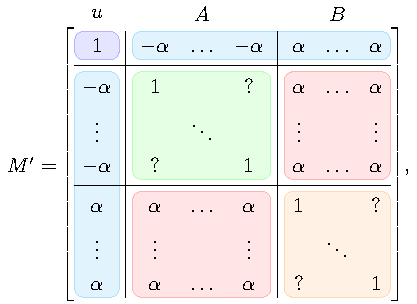
\includegraphics{images/colored-matrix}
    \end{figure}
    \vspace{-0.5em}
    \noindent
    where the $?$ entries can be either $-\alpha$ or $\alpha$.
    Now consider the vector $\bm{v}$ that assigns the value $\alpha$ to $u$, as well as $1 / |A|$ to each vertex in $A$ and $-1/|B|$ to each vertex in $B$.
    By upper bounding all the $?$ entries of $M'$ by $\alpha$, we then obtain 
    \begin{figure}[H]
        \centering
        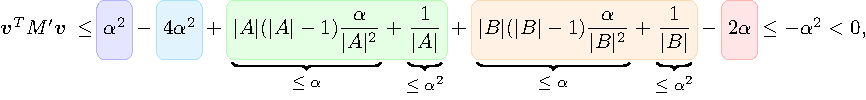
\includegraphics{images/colored-equation}
    \end{figure}
    % \begin{align*}
    %     \bm{v}^T M' \bm{v} 
    %         &\le \alpha^2 - 4\alpha^2 + \underbrace{|A|( |A| - 1) \frac{\alpha}{|A|^2}}_{\le \alpha} + \underbrace{\frac{1}{|A|}}_{\le \alpha^2} + \underbrace{|B|( |B| - 1)\frac{\alpha}{|B|^2}}_{\le \alpha} + \underbrace{\frac{1}{|B|}}_{\le \alpha^2} -\; 2 \alpha  
    %         % &\le \alpha ^2 + \frac{1}{|A|} + \frac{1}{|B|} - 4 \alpha^2 
    %         \le -\alpha^2 < 0,
    % \end{align*}
    \vspace{-0.5em}
    \noindent
    contradicting the positive semidefiniteness of $M$. 
    We conclude that such a configuration cannot exist.
\end{proof}

\begin{figure}[ht]
    \centering
    \includestandalone{tikz/forbidden-configuration}
    \captionsetup{justification=centering, margin=2cm}
    \caption{Forbidden type (ii) configuration}
    \label{fig:forbidden-typeii-config}
\end{figure}

Now we want to prove Theorem \ref{thm:bounded-degree-associated-graph}.
Recall that for a set of equiangular lines, we constructed the associated graph $G$ by choosing an arbitrary set of unit vectors that represents the equiangular set.
Replacing any of these unit vectors $\bm{u}$ by $-\bm{u}$ has the effect of exchanging the neighbours and non-neighbours of $\bm{u}$ in $G$. 
Using the forbidden induced subgraphs of the above lemma, we are going to argue that we can switch some of the vectors to obtain a bounded-degree graph.

\begin{proof}[Proof of Theorem \ref{thm:bounded-degree-associated-graph}]
    Fix $\alpha > 0$.
    Given a set of $n$ equiangular lines in $\R^d$ with pairwise angle $\arccos \alpha$, choose unit vectors $\bm{x}_1, \dots, \bm{x}_n$ along the lines arbitrarily.
    Let $G$ be the associated graph with vertex set $\{ \bm{x}_1, \dots, \bm{x}_n \}$ and an edge between $\bm{x}_i$ and $\bm{x}_j$ whenever $\langle \bm{x}_i, \bm{x}_j \rangle = -\alpha$.
    Let $M_1$, $M_2$ be defined as in Lemma \ref{lem:forbidden-induced-subgraphs}, and let $M = M_2^2 + 2M_2$.
    By Ramsey's theorem, there exists a constant $R = R(M_1, M)$ such that any graph on at least $R$ vertices contains either a clique of size $M_1$ or an independent set of size $M$.
    If $n = |G|\; < R$, we can bound $\Delta (G) \le R$ and are done. 
    (Note that $R$ only depends on $M_1$ and $M$, which in turn only depend on $\alpha$.)
    
    Hence, assume $|G|\; \ge R$. 
    Since $G$ does not contain a clique of size $M_1$ by the lemma, there must be an independent set $S \subseteq V(G)$ of size $M$.

    Consider any vertex $\bm{u} \in V(G) \setminus S$. 
    Let $V_1 = S \cap N_G(\bm{u})$ be the set of neighbours of $\bm{u}$ in $S$, and let $V_2 = S \setminus V_1$. 
    Since both $V_1$ and $V_2$ are contained in the independent set, there are no edges between $V_1$ and $V_2$. 
    By Lemma \ref{lem:forbidden-induced-subgraphs}, one of $V_1, V_2$ must contain fewer than $M_2$ vertices, since otherwise, we would have a forbidden type (ii) configuration.
    In the case where $|V_1|\; > M_2$, we replace $\bm{u}$ by $-\bm{u}$, so that $-\bm{u}$ has at most $M_2$ neighbours in $S$ in the resulting graph.
    After performing this procedure for each $\bm{u} \in V(G) \setminus S$, we may assume that every vertex in $G$ has at most $M_2$ neighbours in $S$.

    We claim that the resulting graph $G$ has maximum degree at most $M_2$.
    Suppose some vertex $\bm{u}$ has degree $d_G(\bm{u}) > M_2$. 
    Let $A \subseteq N_G(\bm{u})$ be a subset of the neighbourhood of size $M_2$. 
    Recall that $\bm{u}$ as well as each vertex in $A$ has at most $M_2$ neighbours in $S$, so 
    \begin{equation*}
        |S \cap N_G(\{ \bm{u}\} \cup A) |\; \le (M_2 + 1) M_2.
    \end{equation*}
    Define $B = S \setminus N_G(\{ \bm{u} \} \cup A)$. 
    Then there are no edges between $A$ and $B$, and 
    \begin{equation*}
        |B|\; \ge |S|\, -\, (M_2 + 1) M_2 = M_2.
    \end{equation*}
    Hence, $\bm{u}, A, B$ forms a forbidden type (ii) configuration, contradicting Lemma \ref{lem:forbidden-induced-subgraphs}.
    We conclude that $\Delta(G)$ is bounded by $M_2$, a constant depending only on $\alpha$.
\end{proof}

% \begin{lemma}
%     The largest clique in $G$ has size at most $\alpha^{-1} + 1$.
% \end{lemma}

% \begin{proof}
%     Consider a clique in $G$ consisting of unit vectors $\bm{x}_1, \dots, \bm{x}_K$, so that $\bm{x}_i ^T \bm{x}_j = -\alpha$ for $i \ne j$.
%     Then we have 
%     \begin{equation*}
%         0 \le \| \bm{x}_1 + \dots + \bm{x}_K \| ^2\; = \sum \limits_{i = 1}^K \underbrace{\bm{x}_i ^T \bm{x}_i}_{= 1} + \sum \limits_{i \ne j} \underbrace{\bm{x}_i^T \bm{x}_j}_{= -\alpha} = K - K(K - 1) \alpha.
%     \end{equation*}
%     Hence, $K \ge K(K - 1) \alpha$, so $K \le \alpha^{-1} + 1$.
% \end{proof}

% \begin{definition}
%     Let $G$ be a graph. 
%     For subsets $A \subseteq X \subseteq V(G)$, define $C_X (A)$ to be the set of vertices in $V(G) \setminus X$ that are adjacent to all vertices in $A$ and to none in $X \setminus A$.
% \end{definition}

\section{Bounding the second eigenvalue multiplicity} 
    \label{section:snd-eigval-multiplicity}
In this section, we prove Theorem \ref{thm:snd-eigval-multiplicity}, which provides the sublinear bound on the second eigenvalue multiplicity.
For any graph $G$ and $\lambda \in \R$, we denote the multiplicity of $\lambda$ as an eigenvalue of $G$ by $m_G(\lambda)$.
If $\lambda$ is not an eigenvalue, then $m_G(\lambda) = 0$.

First of all, let us discuss the necessity of the assumptions of the theorem. 
The restriction on connected graphs cannot be dropped since $\lambda_2$ can be the spectral radius of linearly many small components.  
For instance, the disjoint union of $n / 2$ edges has spectral radius $1$ with \mbox{multiplicity $n/2$}.

The example of the complete graph $K_n$ illustrates that graphs with an unbounded maximum degree need not have sublinear second eigenvalue multiplicity, as $K_n$ has second eigenvalue $-1$ with multiplicity $n - 1$.

Via a slight modification of the proof we are about to discuss, one can show that for any constant $j$, the multiplicity of the $j$-th eigenvalue is $O_{\Delta, j} (n / \log \log n)$ (see \cite{equiangular}).
However, for eigenvalues in the centre of the spectrum, the statement is false.
The following construction found in \cite{equiangularexpository}, in which each vertex of a path of length $l$ is joined with two degree-one vertices, has the eigenvalue $0$ with linear multiplicity.

\begin{figure}[H]
    \centering
    \begin{tikzpicture}
        % Define the vertices with manual positions
        \mynode (v1) at (0, 1) {};
        \mynode (v2) at (0.5, 0) {};
        \mynode (v3) at (1, 1) {};

        \mynode (v4) at (2, 1) {};
        \mynode (v5) at (2.5, 0) {};
        \mynode (v6) at (3, 1) {};

        \mynode (v7) at (4, 1) {};
        \mynode (v8) at (4.5, 0) {};
        \mynode (v9) at (5, 1) {};

        \node[circle, draw=white, fill=white, inner sep=2pt, minimum size=5pt] (x1) at (5.5, 0) {};
        \node at (6.5, 0.5) {\ldots};
        \node[circle, draw=white, fill=white, inner sep=2pt, minimum size=5pt] (x2) at (7.5, 0) {};

        \mynode (v10) at (8, 1) {};
        \mynode (v11) at (8.5, 0) {};
        \mynode (v12) at (9, 1) {};

        \node at (v1) [above = .1cm] {0};
        \node at (v3) [above = .1cm] {0};

        \node at (v4) [above = .1cm] {-1};
        \node at (v6) [above = .1cm] {1};

        \node at (v7) [above = .1cm] {0};
        \node at (v9) [above = .1cm] {0};

        \node at (v10) [above = .1cm] {0};
        \node at (v12) [above = .1cm] {0};
        
        \node at (v2) [below = .1cm] {0};
        \node at (v5) [below = .1cm] {0};
        \node at (v8) [below = .1cm] {0};
        \node at (v11) [below = .1cm] {0};

        % % Draw the edges
        \draw (v1) -- (v2);
        \draw (v3) -- (v2);
        
        \draw (v4) -- (v5);
        \draw (v6) -- (v5);

        \draw (v7) -- (v8);
        \draw (v9) -- (v8);

        \draw (v10) -- (v11);
        \draw (v12) -- (v11);

        \draw (v2) -- (v5);
        \draw (v2) -- (v8);
        \draw (x1) -- (v8);
        \draw (x2) -- (v11);
    \end{tikzpicture}
    \captionsetup{justification=centering, margin=2cm}
    \caption{One of the $0$-eigenvectors of the graph}
    \label{fig:modified-path}
\end{figure}
To see that, consider any vertex $v_i$ on the path, $i \in [l]$.
The vector assigning $1$ to one of the degree-one neighbours of $v_i$, $-1$ to the other and $0$ to all remaining vertices (see Figure \ref{fig:modified-path}) is an eigenvector for the eigenvalue $0$.
These eigenvectors are linearly independent for distinct $i$, so the eigenvalue $0$ has multiplicity at least $l$.

In order to prove the theorem, we first need a few lemmas.

\begin{lemma} \label{lem:bound-size}
    Let $G$ be a graph with $\lambda_2(G) \le 0$. 
    Then $e(G) \le \Delta(G)^2$.
\end{lemma}

\begin{proof}
    Let $n$ = $|G|$, and let $\lambda_1 \ge \dots \ge \lambda_n$ denote the eigenvalues of $G$. We have
    \begin{align*}
        2e(G) = \sum \limits_{i = 1}^n \lambda_i ^2 = \lambda_1^2 + \sum \limits_{i = 2}^n \lambda_i ^2 
        \le \lambda_1^2 + \left( \sum \limits_{i = 2}^n \lambda_i \right)^2 
        = \lambda_1^2 + (-\lambda_1)^2 \le 2 \Delta(G)^2 .
    \end{align*}
    The middle inequality holds because $\lambda_i \le 0$ for all $i \ge 2$.
\end{proof}

\begin{definition}
    An \textit{$r$-net} in $G$ is a subset $U \subseteq V(G)$ such that every vertex in $G$ is within distance $r$ from some vertex in $U$.

    The \textit{$r$-neighbourhood} of a vertex $v$ in $G$, denoted $G_r(v)$, is the subgraph of $G$ induced by all vertices that are at distance at most $r$ from $v$.
\end{definition}

At a very high level, the proof of the theorem proceeds as follows. 
First, we are going to remove a net of small size from our graph. 
We shall see that this significantly reduces the spectral radii of neighbourhoods in $G$ (i.e. the \textit{local spectral radii}), which will allow us to derive a bound on the multiplicity of the second eigenvalue in the remaining graph.
To bound the multiplicity in the original graph, we then use the following observation.

\begin{observation} \label{observation:interlacing}
    Let $G$ be a graph with eigenvalue $\lambda$. 
    Removing $k$ vertices from $G$ does not decrease the multiplicity of $\lambda$ by more than $k$.
\end{observation}

\begin{proof}
    Let $\lambda_1 \ge \dots \ge \lambda_n$ denote the eigenvalues of $G$.
    If we remove one vertex $v$ from $G$, the eigenvalues $\mu_1 \ge \dots \ge \mu_{n - 1}$ of $G - v$ interlace those of $G$:
    \begin{equation*}
        \lambda_1 \ge \mu_1 \ge \lambda_2 \ge \mu_2 \ge \dots \ge \mu_{n - 1} \ge \lambda_n.
    \end{equation*}
    Hence, if the multiplicity of $\lambda$ in $G$ is $m$, its multiplicity in $G - v$ is at least $m - 1$.
    Iterating the argument $k$ times yields the observation.
\end{proof}

The next lemma guarantees the existence of small nets.
\begin{lemma} \label{lem:small-r-net}
    Let $n, r$ be positive integers. Every connected graph $G$ on $n$ vertices has an $r$-net of size at most $\lceil \frac{n}{r + 1} \rceil$
\end{lemma}

\begin{proof}
    We can assume that $G$ is a tree, otherwise consider a spanning tree of $G$.
    We construct an $r$-net of the desired size as follows:
    Pick an arbitrary vertex $v$, and a vertex $w$ with maximum distance from $v$. 
    If $\dist_G (v, w) \le r$, then $\{ v \}$ is an $r$-net and we are done.
    Otherwise, let $u$ be the vertex on the path between $v$ and $w$ at distance $r$ from $w$. 
    We add $u$ to the net and iterate the procedure on the component of $G - u$ that \mbox{contains $v$}. 
    Since the remaining tree has at most $n - (r + 1)$ vertices, this yields an $r$-net of size at most $\lceil \frac{n}{r + 1} \rceil$.
\end{proof}

Removing a net destroys closed walks in a graph and hence reduces the spectral radius.

\begin{lemma} \label{lem:net-removal}
    Let $G$ be a graph, $r \in \N$, and let $H$ be a subgraph obtained from $G$ by deleting an $r$-net. 
    Then 
    \begin{equation*}
        \lambda_1 (H)^{2r} \le \lambda_1 (G)^{2r} - 1.
    \end{equation*}
\end{lemma}

\begin{proof}
    We can assume that $G$ has no isolated vertices because these do not affect the spectral radius.
    For each $v \in V(H)$, the number of closed walks of length $2r$ starting at $v$ is strictly less in $H$ than in $G$. 
    Indeed, in $G$ one can walk from $v$ to a vertex of the $r$-net and back (and possibly walk back and forth along a single edge to reach the length $2r$), and this walk no longer exists in $H$.
    Therefore, $A_H^{2r} \le A_G^{2r} - I$ (padding zeros to extend $A_H$ to a matrix of size $|G| \times |G|$). 
    By the Perron--Frobenius theorem, it follows that 
    \begin{equation*}
        \lambda_1 (H)^{2r} = \lambda_1 ( A_H ^{2r}) \le \lambda_1 ( A_G ^{2r} - I) = \lambda_1 (G)^{2r} - 1.
    \end{equation*}
\end{proof}

The next lemma establishes a connection between the spectrum of a graph and its local spectral radii.
\begin{lemma} \label{lem:local-radii}
    For every graph $G$ and every $r \in \N$, 
    \begin{equation*}
        \sum \limits_{i = 1}^{|G|} \lambda_i (G) ^{2r} \le \sum \limits_{v \in V(G)} \lambda_1 (G_r (v))^{2r}.
    \end{equation*}
\end{lemma}

\begin{proof}
    Recall that 
    \begin{equation*}
        \sum \limits_{i = 1}^{|G|} \lambda_i (G) ^{2r} = \tr A_G^{2r},
    \end{equation*}
    so the left-hand side counts the number of closed walks of length $2r$ in $G$.
    Consider a vertex $v \in V(G)$. 
    A closed walk of length $2r$ starting at $v$ must stay within distance $r$ from $v$, so the number of such walks in $G$ equals the number in $G_r(v)$.
    By Lemma \ref{lem:bounding-walks}, the number of closed walks of length $2r$ in $G_r(v)$ starting at $v$ is at most $\lambda_1(G_r (v))^{2r}$. 
    Hence, the right-hand side is an upper bound for the number of closed walks in $G$, and the inequality follows.
\end{proof}

Now we are ready to prove the theorem, mostly following the version of the proof in \cite{equiangularexpository}.

\begin{proof}[Proof of Theorem \ref{thm:snd-eigval-multiplicity}]
    Let $G$ be a connected graph on $n$ vertices.
    For ease of notation, let $\lambda = \lambda_2(G)$.
    We can assume that $\lambda > 0$ since otherwise $G$ has bounded size by Lemma \ref{lem:bound-size} (and hence also bounded second eigenvalue multiplicity).
    We can also assume that $\Delta \ge 2$, since otherwise $G$ consists only of a single edge.
    
    Define $r = \lfloor c \log \log n \rfloor$ and $s = \lfloor c \log n \rfloor$, where $c = c(\Delta) > 0$ is a sufficiently small constant to be determined later.

    Suppose there is a vertex $v$ with $\lambda_1 (G_{s + 1} (v)) > \lambda$.
    Then Lemma \ref{lem:disjoint-subgraphs} tells us that the spectral radius of $G \setminus G_{s + 2} (v)$ is strictly smaller than $\lambda$; in particular, $\lambda$ is not an eigenvalue of $G \setminus G_{s + 2} (v)$.  
    Recall that by Observation \ref{observation:interlacing}, the multiplicity of $\lambda$ cannot decrease by more than $|G_{s + 2} (v)|$ when removing $G_{s + 2} (v)$. 
    Thus, the multiplicity of $\lambda$ in $G$ is at most 
    \begin{equation*}
        |G_{s + 2} (v)|\; \le 1 + \Delta^{s + 2} \le 1 + \Delta^{c \log n + 2} = 1 + \Delta^2 n^{c \log \Delta} = O(\sqrt{n}),
    \end{equation*}
    if $c$ is chosen to be at most $(2 \log \Delta)^{-1}$.

    Henceforth assume $\lambda_1 (G_{s + 1} (v)) \le \lambda$ for all $v \in V(G)$.
    Let $U$ be an $r$-net of size $\lceil n / (r + 1) \rceil$ in $G$, whose existence is guaranteed by Lemma \ref{lem:small-r-net}, and let $H = G - U$. 
    We wish to bound the multiplicity of $\lambda$ in $H$.
    By Lemma \ref{lem:local-radii},
    \begin{equation*}
        m_H (\lambda) \cdot \lambda^{2s} \le \sum \limits_{i = 1}^{|H|} \lambda_i(H)^{2s} \le \sum \limits_{v \in V(H)} \lambda_1 (H_s (v))^{2s}.
    \end{equation*}

    Furthermore, for every $v \in V(H)$, the vertices in $G_{s + 1} (v) \setminus H_s (v)$ form an $r$-net of $G_{s + 1} (v)$.
    Indeed, starting from any vertex in $G_{s + 1} (v)$, we can walk to a vertex $u \in U$, making at most $r$ steps.
    If $u$ is at distance at most $s + 1$ from $v$ in $G$, we have $u \in G_{s + 1} (v) \setminus H_s (v)$ (note that $u \notin V(H)$ by the definition of $H$).
    Otherwise, the path to $u$ uses a vertex at distance exactly $s + 1$ from $v$, and that vertex is contained in $G_{s + 1} (v) \setminus H_s (v)$.

    For every $v \in V(H)$, it follows by Lemma \ref{lem:net-removal} that 
    \begin{equation*}
        \lambda_1 (H_s (v))^{2r} \le \lambda_1 (G_{s + 1}(v)) ^{2r} - 1 \le \lambda^{2r} - 1.
    \end{equation*}
    Hence,
    \begin{equation*}
        \lambda_1 (H_s (v))^{2s} \le (\lambda^{2r} - 1)^{\frac{s}{r}}.
    \end{equation*}
    Combining the inequalities, we obtain
    \begin{equation*}
        m_H (\lambda) \cdot \lambda^{2s} \le n (\lambda^{2r} - 1)^{\frac{s}{r}}.
    \end{equation*}
    Thus, using the inequality $1 + x \le e^x$, 
    \begin{align*}
        m_H (\lambda) &\le \frac{n}{\lambda^{2s}} (\lambda^{2r} - 1)^{\frac{s}{r}} 
            = n \cdot \left ( \frac{1}{\lambda^{2r}} ( \lambda^{2r} - 1) \right) ^{\frac{s}{r}} \\ 
        &= n \cdot (1 - \lambda^{-2r})^{\frac{s}{r}} 
            \le n \cdot e ^{-\frac{s}{r} \cdot \lambda^{-2r}} 
            \le n \cdot e^{-\sqrt{\log n}}.
    \end{align*}
    For the last inequality, we have used that $\lambda \le \lambda_1 \le \Delta$ and therefore,
    \begin{align*}
        \frac{s}{r} \cdot \lambda^{-2r} &\ge \frac{c \log n - 1}{c \log \log n} \cdot \Delta^{-2 c \log \log n} \\ 
        &\ge \frac{\log n}{2 \log \log n} \cdot (\log n)^{-2 c \log \Delta} = \frac{(\log n)^{1 - 2c \log \Delta}}{2 \log \log n} \ge \sqrt{\log n},
    \end{align*}
    provided that $c$ is chosen smaller than $(4 \log \Delta)^{-1}$ and $n$ is large enough.

    Finally, we apply Observation \ref{observation:interlacing}. 
    Since $H$ is obtained from $G$ by removing an $r$-net consisting of at most $\lceil n / (r + 1) \rceil$ vertices, 
    \begin{equation*}
        m_G(\lambda) \le m_H(\lambda) + \left \lceil \frac{n}{r + 1} \right \rceil \le \frac{n}{e^{\sqrt{\log n}}} + \left \lceil \frac{n}{c \log \log n} \right \rceil
            = O \Big(\frac{n}{\log \log n} \Big),
    \end{equation*}
    which completes the proof.
\end{proof}

Since no construction of a bounded-degree graph with second eigenvalue multiplicity \sloppy $\Theta(n / \log \log n)$ is known, the authors of \cite{equiangular} conjectured that the bound in Theorem \ref{thm:snd-eigval-multiplicity} can be improved.
Observe that any improvement on the size of an $r$-net immediately yields a stronger bound on the second eigenvalue multiplicity by the same proof. 
In the conclusion of the paper \cite{equiangular}, it is remarked that the existence of smaller nets can be guaranteed among expander graphs.\footnote{Here we use a slightly different notion of expansion than in Section \ref{section:cheeger}, considering neighbouring vertices instead of edge boundaries.}

% Now fix an $n$-vertex graph $G$ with maximum degree at most $\Delta$. 
% Suppose $G$ is an expander graph in the sense that $|N_G(A)|\; \ge (1 + \varepsilon) |A|$ for all $A \subseteq V(G)$ with $|A|\; \le \frac{n}{2}$ for some $\varepsilon > 0$.


\begin{lemma}
    Let $G$ be a graph of order $n$.
    Suppose there exists $\varepsilon > 0$ such that $|N_G(A)|\; \ge (1 + \varepsilon) |A|$ for all $A \subseteq V(G)$ with $|A|\; \le \frac{n}{2}$.
    Then, for every $r \in \N$, the graph $G$ contains an $r$-net of size at most \mbox{$n / (1 + \varepsilon)^{\lfloor r / 2 \rfloor}$}.
\end{lemma}

\begin{proof}
    Let $S \subseteq V(G)$ be a maximal $r$-separated set in $G$, that is, a maximal subset of the vertices in $G$ such that any two vertices in $S$ have distance at least $r + 1$.
    Then $S$ is an $r$-net in $G$: Suppose there was a vertex $v$ not within distance at most $r$ from any vertex \mbox{in $S$}. 
    Then $S \cup \{ v\}$ would form a larger $r$-separated set, contradicting the maximality \mbox{of $S$}.

    It remains to show that $|S|\; \le n / (1 + \varepsilon)^{\lfloor r / 2 \rfloor}$.
    For any vertex $v \in S$, consider its $\lfloor r /2 \rfloor$-neighbourhood $G_{\lfloor r /2 \rfloor} (v)$.
    Due to the expansion property, 
    \begin{equation*}
        |G_{\lfloor r /2 \rfloor} (v)|\; \ge (1 + \varepsilon) ^{{\lfloor r / 2 \rfloor}}.
    \end{equation*}
    By the definition of $S$, the ${\lfloor r / 2 \rfloor}$-neighbourhoods of the vertices in $S$ are necessarily disjoint.
    We conclude that $n \ge |S| \cdot (1 + \varepsilon) ^{{\lfloor r / 2 \rfloor}}$, as claimed.
\end{proof}

Now let $G$ be an expander graph as in the lemma.
Let $r = \lfloor c \log \log n \rfloor$ as in the proof of Theorem \ref{thm:snd-eigval-multiplicity},
and suppose $U$ is an $r$-net of size at most $n / (1 + \varepsilon)^{\lfloor r / 2 \rfloor}$ in $G$. 
We have 
\begin{equation*}
    (1 + \varepsilon)^{\lfloor r / 2 \rfloor} \ge (1 + \varepsilon)^{ c \log \log n} = (\log n)^{c \log (1 + \varepsilon)} \ge (\log n)^\alpha
\end{equation*}
for any $\alpha \le c \log (1 + \varepsilon)$.
Hence, $|U|\; \le n / (\log n)^\alpha$, 
and we obtain:

\begin{corollary}
    Fix $\Delta > 0$ and $\varepsilon > 0$.
    Let $G$ be an $n$-vertex graph with maximum degree at most $\Delta$, and suppose $G$ satisfies $|N_G(A)|\; \ge (1 + \varepsilon) |A|$ for all $A \subseteq V(G)$ with $|A|\; \le \frac{n}{2}$.
    Then there exists a constant $\alpha$ depending only on $\Delta$ and $\varepsilon$ such that
    \begin{equation*}
        m_G (\lambda_2) \le O_{\Delta} \left(\frac{n}{(\log n)^\alpha} \right).
    \end{equation*}
\end{corollary}

\begin{remark}
    The authors of \cite{equiangular} even claim that for an expander graph as in the corollary, the second eigenvalue multiplicity is at most $O_{\Delta, \varepsilon}(n / \log n)$. 
    However, this does not follow directly from their proof, so we think that it is an inaccuracy.
\end{remark}

It remains an intriguing problem to determine the optimal bounds for general graphs in Theorem \ref{thm:snd-eigval-multiplicity}.
The currently best-known lower bound comes from a family of graphs with maximum degree $4$ and second eigenvalue multiplicity at least $\sqrt{n / \log_2 n}$ \mbox{(see \cite{snd-eigval-lower-construction}).}
Therefore, the following question suggests itself:
\begin{question}
    Does there exist a constant $\alpha > 0$, such that every $n$-vertex connected graph with maximum degree at most $\Delta$ has second eigenvalue multiplicity at most \mbox{$O_\Delta (n^{1 - \alpha})$}?
\end{question}
Despite the relatively large gap between the lower bound constructions and the upper bounds, and even though the paper of Jiang et al. \cite{equiangular} appears to have initiated some research in that direction, no significantly stronger result has been found for general graphs yet.
However, McKenzie, Rasmussen, and Srivastava \cite{mckenzie2023supportclosedwalkssecond} established the following improved bound for regular graphs.
\begin{theorem}[\cite{mckenzie2023supportclosedwalkssecond}, Theorem 4.1]
    Let $d \in \N$. Every $d$-regular graph $G$ on $n$ vertices satisfies
    \begin{equation*}
        m_G (\lambda_2) = O_d \bigg( \frac{n \log \log n }{\log ^{1/5} n}\bigg).
    \end{equation*}
\end{theorem}

On a high level, their proof strategy is similar to that from \cite{equiangular} for Theorem \ref{thm:snd-eigval-multiplicity}. 
The main difference is that in \cite{mckenzie2023supportclosedwalkssecond}, they analysed random walks in regular graphs and showed that a typical random walk uses a "large" number of vertices. 
They concluded that by removing a small set of vertices chosen randomly, many of these walks are destroyed, which they could in turn use to derive a bound on the second eigenvalue multiplicity of the remaining graph.
The improvement comes from the fact that they were able to delete only $O (n \log \log n / \log ^{1/5} n)$ vertices, as opposed to $O(n / \log \log n)$ vertices in \cite{equiangular}.

The technique used in \cite{equiangular} and \cite{mckenzie2023supportclosedwalkssecond} to estimate $m_G(\lambda_2)$ is also known as the \textit{trace method} or \textit{moment method}. 
In general, one starts by estimating the number of closed walks of length $2k$ in a graph $G$. 
Recall that this number is equal to 
\begin{equation*}
    \tr A_G^{2k} = \sum_{i = 1}^{|G|} \lambda_i^{2k}.
\end{equation*}
Now one relies on the idea that for large $k$, the sum on the right-hand side will be dominated by $\lambda_1^{2k} + m_G(\lambda_2) \cdot \lambda_2^{2k}$, which can be used to bound $\lambda_2$ or $m_G (\lambda_2)$.

Naturally, these estimates allow for some margin of error. 
Specifically, Haiman, Schildkraut, Zhang, and Zhao \cite{snd-eigval-lower-construction} demonstrated that the proof of Theorem \ref{thm:snd-eigval-multiplicity} can be slightly modified to show that there are at most $O(n / \log \log n)$ eigenvalues within the interval $[(1 - 1/\log n) \lambda_2, \lambda_2]$.
Furthermore, they constructed a family of connected bounded-degree graphs matching this bound up to a constant factor. 
This can be seen as an indication that substantially stronger techniques may be necessary to push the upper bounds for general graphs further.

\section{Separable graphs}
Since the currently known upper bounds on the second eigenvalue multiplicity of general graphs do not appear optimal yet, it is also of interest to consider special classes of graphs. 
In this section, we show stronger bounds than in Theorem \ref{thm:snd-eigval-multiplicity} for so-called \textit{separable graphs}.
The key concept that we shall need is the following.

\begin{definition}
    Let $G$ be a graph on $n$ vertices. 
    A subset $S \subseteq V(G)$ is a \textit{(balanced) separator} if there exists a partition $V(G) \setminus  S =  A \cup B$ such that $|A|, |B|\;\le \frac{2n}{3}$ and $G$ has no edges between $A$ and $B$.
\end{definition}

A planar graph is a graph that can be drawn in the plane in such a way that no two edges intersect (for a formal definition, refer to \cite[Chapter 4]{diestel}). 
The famous planar separator theorem due to Lipton and Tarjan \cite{liptontarjan} states that every planar graph on $n$ vertices has a separator of size at most $O(\sqrt{n})$. 
This result is optimal up to constant factors, as demonstrated by the $n \times n$ grid graph (cf. Figure \ref{fig:separator-grid}).

\begin{figure}[ht]
    \centering
    \begin{tikzpicture}
        \draw[fill=green!10, draw=green!30, rounded corners] (0.5, 0.5) rectangle (1.9, 4.3);
        \draw[fill=blue!10, draw=blue!30, rounded corners] (2.1, 0.5) rectangle (2.7, 4.3);
        \draw[fill=red!10, draw=red!30, rounded corners] (2.9, 0.5) rectangle (4.3, 4.3);

        \foreach \i in {1, 2, 3, 4, 5} {
            \foreach \j in {1, 2, 3, 4, 5} { 
                \mynode (v\i\j) at (0.8 * \i, 0.8 * \j) {};
            }
        }

        \foreach \x in {1,2,3,4,5} {
            \foreach \y in {1,2,3,4,5} {
                \ifnum\x<5
                    \draw (v\x\y) -- (v\the\numexpr\x+1\relax\y);
                \fi
                \ifnum\y<5
                    \draw (v\x\y) -- (v\x\the\numexpr\y+1\relax);
                \fi
            }
        }

        % Label the rectangles
        \node at (1.2,0) {$A$};
        \node at (2.4,0) {$S$};
        \node at (3.6,0) {$B$};
    \end{tikzpicture}
    \captionsetup{justification=centering, margin=2cm}
    \caption{A balanced separator of the $5 \times 5$ grid}
    \label{fig:separator-grid}
\end{figure}

Motivated by the planar separator theorem, we consider general classes of graphs with "small" separators and bound the second eigenvalue multiplicity of such graphs.

\begin{definition}
    Let $\mathcal{G}$ be a hereditary class of graphs (that is, closed under taking induced subgraphs), 
    and let $f : \N \rightarrow \R^+$ be a function.
    We say that the graphs in $\mathcal{G}$ are \textit{$f$-separable} if any graph $G \in \mathcal{G}$ has a balanced separator of size $O(f(|G|))$.
\end{definition}

\begin{theorem} \label{thm:separable-snd-eigval-mult}
    Let $\Delta \in \N$ and $f : \N \rightarrow \R^+$ be an increasing function satisfying \mbox{$f(\frac{2}{3}n) \le \alpha f(n)$} for some $\alpha < 1$ and all $n \in \N$.
    Let $\mathcal G$ be a hereditary class of $f$-separable graphs with maximum degree at most $\Delta$. 
    Then all connected graphs in $\mathcal G$ have second eigenvalue multiplicity at most $O_{\Delta}(f)$.
\end{theorem}

\begin{proof}
    By the theorem's hypothesis, there exists a constant $R$ such that any $n$-vertex graph in $\mathcal{G}$ has a separator of size at most $R f(n)$.
    
    Let $G \in \mathcal G$ be a graph with $n$ vertices.
    As usual, we denote the eigenvalues of $G$ by $\lambda_1 \ge \dots \ge \lambda_n$.
    We use induction on $n$ to show that 
    \begin{equation*}
        m_G (\lambda_2) \le \frac{R(\Delta + 1)}{1 - \alpha} f(n).
    \end{equation*}    
    The bound trivially holds for $n = 2$.
    %\footnotemark
    (Note that we must have $Rf(2) \ge 1$.)%, as a separator cannot be empty in a connected graph.)
    %\footnotetext{Note that a separator cannot be empty in a connected graph, so we must have $Rf(2) \ge 1$.}
    
    Now let $n$ be fixed and suppose the theorem holds for all graphs with fewer than $n$ vertices. 
    Let $S \subseteq V(G)$ be a separator in $G$ of size $k\, \le R f(n)$ and define $G' = G - S$.
    If $m_G (\lambda_2) \le (\Delta + 1)k$, we are done. 
    Hence assume $m_G (\lambda_2) = m + k$ for some $m \ge \Delta k + 1$.
    % By Observation \ref{observation:interlacing}, the multiplicity of $\lambda_2$ in $G'$ is at least $m$.
    Let $\mu_1 \ge \dots \ge \mu_{n - k}$ denote the eigenvalues of $G'$.
    By the Cauchy interlacing theorem, we have 
    \begin{equation*}
        \lambda_i \ge \mu_i \ge \lambda_{i + k}, \ \ i \in [n - k].
    \end{equation*}
    In particular, as $\lambda_2 = \dots = \lambda_{m + k + 1}$,
    \begin{equation*}
        \lambda_2 = \mu_2 = \dots = \mu_{m + 1},
    \end{equation*}
    so the multiplicity of $\lambda_2$ in $G'$ is at least $m$, and $G'$ has at most one eigenvalue larger \mbox{than $\lambda_2$}.
    
    Since $G'$ has at most $\Delta k < m$ components, there is one, $C$ say, in which the eigenvalue $\lambda_2$ occurs more than once.
    By the Perron--Frobenius theorem, $\lambda_2$ cannot be the largest eigenvalue \mbox{of $C$}. 
    It follows that $\lambda_2$ is the second-largest eigenvalue of $C$.
    Moreover, by Lemma \ref{lem:disjoint-subgraphs}, no other component of $G'$ has $\lambda_2$ as an eigenvalue.
    Generously bounding $k \le (\Delta + 1)k$, we conclude that
    \begin{equation*}
        m_G(\lambda_2) \le k + m_C(\lambda_2) \le (\Delta + 1) k + m_C (\lambda_2).
    \end{equation*}
    Recall that $|C|\, \le \frac{2}{3}n$. 
    By the induction hypothesis, the latter summand is at most 
    \begin{equation*}
         \frac{R(\Delta + 1)}{1 - \alpha} f \Big( \frac{2}{3}n \Big).
    \end{equation*}
    Thus we obtain 
    \begin{align*}
        m_G( \lambda_2 ) &\le (\Delta + 1)k + \frac{R(\Delta + 1)}{1 - \alpha} f \Big( \frac{2}{3}n \Big) \\ 
        &\le R(\Delta + 1) f(n) + \frac{\alpha R (\Delta + 1)}{1 - \alpha} f(n) = \frac{R (\Delta + 1)}{1 - \alpha} f(n),
    \end{align*}
    as desired.
\end{proof}

\begin{remark}
    By the planar separator theorem, the above result provides a bound of $O_\Delta (\sqrt{n})$ for the second eigenvalue multiplicity of a connected planar graph on $n$ vertices.
    Interestingly, this is still far from the truth: In \cite{planarmultiplicty} it was shown that for such a graph, $m_G(\lambda_2) \le \Delta(G)$.
\end{remark}

To exhibit specific graph classes for which Theorem \ref{thm:separable-snd-eigval-mult} asymptotically improves existing results, we cite the following result by Alon, Seymour, and Thomas, which extends the planar separator theorem to graphs with a fixed forbidden minor.
\begin{theorem}[{\cite[(1.3)]{separatortheoremfornonplanargraphs}}]
    Let $H$ be an arbitrary graph on $h$ vertices. 
    Every $n$-vertex graph $G$ without an $H$-minor has a separator of size at most $h^{\frac{3}{2}} n^{\frac{1}{2}}$.
\end{theorem}

Using Theorem \ref{thm:separable-snd-eigval-mult} we deduce:
\begin{corollary}
    Let $\Delta \in \N$, and let $H$ be a fixed graph on $h$ vertices. 
    Let $\mathcal G$ be a family of connected graphs with maximum degree at most $\Delta$ that do not contain $H$ as a minor. 
    Then the second eigenvalue multiplicity of any graph $G \in \mathcal G$ on $n$ vertices is at most $O_{\Delta, h}(\sqrt{n})$.
\end{corollary}

The last proposition of this chapter states that expander graphs do not have small separators.
This implies that any graph for which Theorem \ref{thm:separable-snd-eigval-mult} yields an improvement over Theorem \ref{thm:snd-eigval-multiplicity} must be sufficiently non-expanding.

\begin{proposition}
    Let $G$ be an $n$-vertex graph, and suppose $G$ satisfies $N_G(A) \ge (1 + \varepsilon) |A|$ for all $A \subseteq V(G)$ with $|A|\; \le n/2$ for some $\varepsilon > 0$.
    Let $S$ be a balanced separator in $G$. 
    Then 
    \begin{equation*}
        |S| \; \ge \frac{\varepsilon n}{3(1 + \varepsilon )}.
    \end{equation*}
\end{proposition}

\begin{proof}
    Consider a partition $A \cup B$ of $V(G) \setminus S$ such that $|A|, |B|\; \le 2n/3$ \mbox{and $e(A, B) = 0$}.
    We can assume that $|A|\; \le |B|$, so in particular $|A|\; \le n/2$.
    Then $|A|\, +\, |S|\; \ge n/3$.
    Clearly, we have $N_G(A) \setminus A \subseteq S$. 
    Hence, 
    \begin{equation*}
        |S|\; \ge |N_G(A) \setminus A|\; \ge \varepsilon |A|.
    \end{equation*}
    It follows that 
    \begin{equation*}
        \frac{n}{3} \le |S| + |A|\; \le (1 + \varepsilon^{-1}) |S|,
    \end{equation*}
    and the claimed inequality is obtained by solving for $|S|$.
\end{proof}

More about the connection between expanders and separators can be found in the survey \cite{krivelevich}.
\chapter{The Sensitivity Conjecture}

This chapter presents a surprising application of spectral graph theory to a long-standing open problem in theoretical computer science: the Sensitivity Conjecture. 
The problem is concerned with the relationship between two different complexity measures of Boolean functions, and has connections to the combinatorics of induced subgraphs of the hypercube.

\section{Boolean functions and complexity measures}
A \textit{Boolean function} is a function $f: \{0, 1\}^n \rightarrow \{0, 1 \}$.
The values (or \textit{bits}) $0$ and $1$ are usually interpreted as truth values \textit{false} and \textit{true}, respectively.
Simple examples of Boolean functions include the logical AND, which can be encoded as \begin{equation*}
    f(x, y) = xy,
\end{equation*} 
the logical OR 
\begin{equation*}
    f(x,y) = x + y - xy,
\end{equation*}
and the negation 
\begin{equation*}
    f(x) = 1 - x.
\end{equation*}
Computational complexity theory is the study of the inherent hardness of computational tasks. 
In particular, this involves establishing lower bounds on the time (or space) needed to compute a given Boolean function on all input vectors, regardless of the algorithm chosen. 
However, for many practically relevant examples (including all NP-complete problems), there is a significant gap between these lower bounds and the best-known algorithms.
In order to obtain a better understanding of the computational hardness of Boolean functions, various complexity measures have been introduced and studied.
%
% The central question with regard to Boolean functions, as phrased by Jukna in \cite{booleanfunctioncomplexity}, is: 
%
% \begin{quote}
%     Given a Boolean function, how many of these simplest operations do we need to compute the function on all input vectors?
% \end{quote}
%
% In order to establish meaningful bounds on the complexity of Boolean functions, various complexity measures have been introduced and studied. 
We are interested in the relation between two of them, namely \textit{sensitivity} and \textit{block sensitivity}.

For any $\bm{x} \in \{0, 1\}^n$ and $S \subseteq [n]$, we denote by $\bm{x}^S$ the vector obtained from $\bm{x}$ by flipping all bits in $S$.

\begin{definition}
    Let $f: \{0, 1\}^n \rightarrow \{0, 1 \}$ be a Boolean function. 
    For any $\bm{x} \in \{0, 1\}^n$, the \textit{local sensitivity} $s(f, \bm{x})$ of $f$ on the input $\bm{x}$ is defined as the number of indices $i \in [n]$ such that $f(\bm{x}) \ne f(\bm{x}^{\{i \}} )$.
    The \textit{sensitivity} $s(f)$ of $f$ is 
    \begin{equation*}
        s(f) = \max \limits_{\bm{x} \in \{0, 1\}^n} s(f, \bm{x}).
    \end{equation*}

    Similarly, the \textit{local block sensitivity} $bs(f, \bm{x})$ of $f$ on the input $\bm{x}$ is defined as the maximum number $k$ of pairwise disjoint blocks $B_1, \dots, B_k \subseteq [n]$ such that $f(\bm{x}) \ne f(\bm{x}^{B_i})$ for each $i \in [k]$.
    The \textit{block sensitivity} $bs(f)$ of $f$ is 
    \begin{equation*}
        bs(f) = \max \limits_{\bm{x} \in \{0, 1\}^n} bs(f, \bm{x}).
    \end{equation*}
\end{definition} 

As the name indicates, sensitivity and block sensitivity measure how sensitive a Boolean function is with respect to local changes in the input.
Since the blocks $B_i$ in the definition of block sensitivity can be chosen as $B_i = \{i \}$, it is clear that $bs(f) \ge s(f)$.
On the other hand, the so-called \textit{Sensitivity Conjecture}, posed by Nisan and Szegedy \cite{nisanszegedy} in the early 1990's, suggested that $bs(f)$ was bounded from above by a polynomial of $s(f)$.

\begin{conjecture}[Sensitivity Conjecture]
    There exists a constant $C > 0$ such that for every Boolean function $f$, 
    \begin{equation*}
        bs(f) \le s(f)^C.
    \end{equation*}
\end{conjecture}

We say that two complexity measures $s_1$ and $s_2$ are \textit{polynomially related} if there exist polynomials $p_1, p_2$ such that 
\begin{equation*}
    s_1(f) \le p_2(s_2(f)) \ \text{ and } \ s_2(f) \le p_1(s_1(f))
\end{equation*}
for all Boolean functions $f$.

It has been known that the block sensitivity is polynomially related to various other complexity measures of Boolean functions, such as \textit{certificate complexity}, \textit{decision tree complexity}, and the \textit{degree} of a representing polynomial (for details, see the survey \cite{buhrmanndewolf}).
Hence, a positive resolution of the Sensitivity Conjecture would mean that the sensitivity falls in the same category of polynomially related complexity measures.

Despite the efforts of numerous researchers, very little progress has been made for almost thirty years, which is why the Sensitivity Conjecture was considered one of the outstanding open problems in theoretical computer science.
It was not until 2019 that Huang \cite{sensitivity} finally achieved a breakthrough and settled the conjecture.
His proof uses methods of spectral graph theory and is notable for its brevity and elegance.

\section{Boolean functions as real polynomials}
Let $f: \{0, 1\}^n \rightarrow \{0, 1 \}$ be a Boolean function. 
We say that a polynomial $p: \R^n \rightarrow \R$ \textit{represents} $f$ if $p(\bm{x}) = f(\bm{x})$ for all $\bm{x} \in \{0, 1\}^n$.
Any Boolean function $f: \{0, 1\}^n \rightarrow \{0, 1 \}$ can be represented as a real polynomial in $\R^n$.
In fact, such a polynomial $p$ can be explicitly obtained by summing over the values taken by $f$ multiplied by indicator polynomials:
\begin{equation*}
    p(\bm{t}) = \sum \limits_{\bm{x} \in \{0, 1\}^n} f(\bm{x})  \prod \limits_{i: \bm{x}_i = 1} \bm{t}_i \prod \limits_{i: \bm{x}_i = 0} (1 - \bm{t}_i  ).
\end{equation*}
This polynomial is multilinear (that is, no monomial contains a variable raised to a power greater than 1), and if we restrict ourselves to multilinear polynomials, the representation of $f$ becomes unique:

\begin{lemma}
    Let $p, q : \R^n \rightarrow \R$ be multilinear polynomials that both represent $f$. Then $p = q$. 
\end{lemma}

\begin{proof}
    Suppose $p \ne q$, and let $r = p - q$, so that $r$ is not the zero polynomial. 
    Consider a subset of indices $S \subseteq [n]$ of minimal size and a coefficient $\alpha \ne 0$ such that that 
    \begin{equation*}
        \alpha \prod \limits_{i \in S} \bm{x}_i
    \end{equation*}
    is a monomial (of minimal degree) in $r$.
    Let $\bm{x} \in \{0, 1\}^n$ such that $\bm{x}_i = 1$ if $i \in S$, and $\bm{x}_i = 0$ otherwise.
    Since $S$ was chosen to have minimal size and $p, q$ are multilinear, all other monomials of $r$ take the value $0$ on $\bm{x}$.
    But this implies 
    \begin{equation*}
        r(\bm{x}) = \alpha \ne 0 = p(\bm{x}) - q(\bm{x}),
    \end{equation*}
    a contradiction.
\end{proof}

In light of this lemma, one can define the \textit{degree} of a Boolean function $f$, denoted $\deg(f)$, as the degree of the unique multilinear real polynomial \mbox{representing $f$}. 
Recall that in the case of a multilinear polynomial $p$, the degree of $p$ is just the maximum number of distinct variables occurring in any monomial in $p$.

Similarly to sensitivity and block sensitivity, the degree is an important complexity measure of a Boolean function. 
Degree and block sensitivity have been shown to be polynomially related (see \cite{buhrmanndewolf}).
In particular, Tal \cite{tal} established the following bound, improving on an earlier result by Nisan and Szegedy \cite{nisanszegedy}.
\begin{theorem} \label{thm:bs-lt-deg}
    For any Boolean function $f$, 
    \begin{equation*}
        bs(f) \le \deg (f)^2.
    \end{equation*}
\end{theorem}

Furthermore, Gotsman and Linial \cite{gotsmanlinial} have found the following remarkable equivalence, providing a bedrock for Huang's later work.

\begin{theorem} \label{thm:sensitivity-equivalence}
    For any increasing function $h: \N \rightarrow \R$, the following statements are equivalent:
    \begin{enumerate}
        \item For any induced subgraph $H$ of the $n$-dimensional hypercube $Q_n$ with $|H|\; \ne 2^{n - 1}$, we have
            \begin{equation*}
                \max \{\Delta(H), \Delta(Q_n - H) \} \ge h(n).
            \end{equation*}
        \item For any Boolean function $f$, we have $s(f) \ge h(\deg(f))$.
    \end{enumerate}
\end{theorem}

The proof of Theorem \ref{thm:sensitivity-equivalence} in \cite{gotsmanlinial} requires Fourier analysis, so we are only going to sketch how (i) can be transformed into an equivalent statement concerning Boolean functions.
The attentive reader may have noticed that the domain of a Boolean function is precisely the vertex set of an $n$-dimensional hypercube. 
Hence, we can associate any induced subgraph $H$ of $Q_n$ with a Boolean function $g: \{0, 1\}^n \rightarrow \{ 0 , 1\}$, such that
\begin{equation*}
    g(\bm{x}) = 1 \ \Longleftrightarrow \ \bm{x} \in V(H).
\end{equation*}
Then we have $d_H(\bm{x}) = n - s(g, \bm{x})$, and the same holds for all $\bm{x} \in V(Q_n - H)$.
Furthermore, note that the condition $|H| \; \ne 2^{n - 1}$ implies that $g$ is unbalanced, i.e. $|g^{-1} (\{0\})|\; \ne |g^{-1} (\{1\})|$.
Therefore, (i) is equivalent to the following statement: 

\begingroup
    \itshape
    \begin{itemize}[font=\upshape]
        \item[(i')] For any unbalanced Boolean function $g$, there exists an input $\bm{x}$ such that 
            \begin{equation*}
                s(g, \bm{x}) \le n - h(n).
            \end{equation*}
    \end{itemize}
\endgroup

The two theorems above show that to verify the Sensitivity Conjecture, it is sufficient to prove statement (i) of Theorem \ref{thm:sensitivity-equivalence} for a suitable function $h$.
In \cite{gotsmanlinial}, the authors already suggested that $h(n)$ might be chosen as $\sqrt{n}$.

\section{The proof of the Sensitivity Conjecture}
    \label{section:sensitivity}

The main result obtained by Huang can be stated as follows:

\begin{theorem}[{\cite[Theorem 1.1]{sensitivity}}] \label{thm:induced-subgraphs}
    Let $n \in \N$, and let $H$ be an induced subgraph of the hypercube $Q_n$ on $2^{n - 1} + 1$ vertices. 
    Then $\Delta(H) \ge \sqrt{n}$. 
\end{theorem}

\begin{remark}
    The vertices of $Q_n$ with an even number of $1$-entries form an independent set in $Q_n$, and hence an induced subgraph with maximum degree $0$.
    The above theorem implies that for any induced subgraph with only one more vertex, the maximum degree jumps to at least $\sqrt{n}$.

    On the other hand, Chung, Füredi, Graham, and Seymour \cite{inducedsubgraphsofthecube} constructed an induced subgraph of $Q_n$ on $2^{n - 1} + 1$ vertices with maximum degree at most $\left \lceil \sqrt{n} \right \rceil$, so the bound of the theorem is sharp.
\end{remark}

Note that the theorem implies statement (i) of Theorem \ref{thm:sensitivity-equivalence}.
First, the lower bound on the maximum degree holds for all induced subgraphs of size at least $2^{n - 1} + 1$, as the maximum degree cannot decrease when more vertices are added.
Secondly, if $H$ is an induced subgraph of $Q_n$ with $|H|\; \ne 2^{n - 1}$, then either $H$ or $Q_n - H$ has at least $2^{n - 1} + 1$ vertices, and hence maximum degree at least $\sqrt{n}$.
As a consequence, we immediately have the following corollary.

\begin{corollary} \label{cor:sf-deg}
    For any Boolean function $f$, we have 
    \begin{equation*}
        s(f) \ge \sqrt{\deg(f)}.
    \end{equation*}
\end{corollary}

Combining the inequalities from Corollary \ref{cor:sf-deg} and Theorem \ref{thm:bs-lt-deg}, this confirms the Sensitivity Conjecture.

\begin{theorem}[Sensitivity Theorem]
    For any Boolean function $f$,
    \begin{equation*}
        bs(f) \le s(f)^4.
    \end{equation*}
\end{theorem}

\begin{remark}
    It is not known whether the exponent $4$ on the right-hand side is optimal. 
    However, Ambainis and Sun \cite{newseparation} constructed Boolean functions $f$ with $bs(f) = \frac{2}{3} s(f)^2 - \frac{1}{3} s(f)$, showing that there is at least a quadratic separation between block sensitivity and sensitivity.
\end{remark}

We are now going to present Huang's proof of Theorem \ref{thm:induced-subgraphs}.
Consider the sequence $(A_n)_{n \in \N}$ of $2^n \times 2^n$ matrices defined as follows:
\begin{equation*}
    A_1 = \begin{bmatrix}
        0 & 1 \\ 1 & 0
    \end{bmatrix}, \ \ \ 
    A_{n + 1} = \begin{bmatrix}
        A_n & I_n \\ I_n & -A_n
    \end{bmatrix}.
\end{equation*}

Recalling our discussion of the hypercube in Example \ref{ex:special_spectra}, we see that by flipping every ($-1$) entry of $A_n$ to $1$, we obtain precisely the adjacency matrix of $Q_n$. 
In other words, the matrix $A_n$ is a signed adjacency matrix of $Q_n$, which means that $A_n$ is symmetric, $(A_n)_{ij} = \pm 1$ whenever there is an edge between $i$ and $j$, and $(A_n)_{ij} = 0$ otherwise. 

The matrices $A_n$ have the following nice property:

\begin{lemma} \label{lem:hypercube-matrices}    
    The matrices $A_n$ have the eigenvalues $\pm \sqrt{n}$, both with multiplicity $2^{n - 1}$.
\end{lemma}

\begin{proof}
    We claim that $A_n^2 = nI$ for all $n \in \N$. 
    This can be seen by induction.
    For $n = 1$, we have $A_1 ^2 = I$, so assume that the equality holds for a fixed $n$. 
    Then 
    \begin{equation*}
        A_{n + 1}^2 
        = \begin{bmatrix}
            A_n & I \\ I & -A_n
        \end{bmatrix}^2
        = \begin{bmatrix}
            A_n ^2 + I & 0 \\
            0 & A_n^2 + I
        \end{bmatrix}
        = (n + 1)I.
    \end{equation*}
    All eigenvalues of $nI$ are $n$, so the eigenvalues of $A_n$ must be $\sqrt{n}$ or $-\sqrt{n}$.
    Since $\tr A_n = 0$, both have to occur with equal multiplicity, that is, with multiplicity $2^{n - 1}$.
\end{proof}

The next lemma generalises the fact that the largest eigenvalue of the adjacency matrix of a graph is not larger than its maximum degree. 

% Let $H$ be a graph, and let $A$ be a symmetric matrix whose rows and columns are indexed by $V(H)$. 
% We say that $A$ \textit{represents} the graph $H$ if for all $u, v \in V(H)$, $A_{uv} \ne 0$ if and only if $uv \in E(H)$.
% The next lemma generalizes the fact that the largest eigenvalue of the adjacency matrix of a graph is not larger than its maximum degree. 

\begin{lemma} \label{lem:maxdeg-sensitivity}
    Let $H$ be a graph on $m$ vertices.
    Suppose $A$ is a symmetric matrix with entries in $\{-1, 0, 1\}$ whose rows and columns are indexed by $V(H)$, such that $A_{vw} = 0$ whenever $v$, $w$ are non-adjacent in $H$.
    Then
    \begin{equation*}
        \Delta(H) \ge \lambda_1(A).
    \end{equation*}
\end{lemma}

\begin{proof}
    Let $\lambda_1 := \lambda_1(A)$, and let $\bm{v}$ be a corresponding eigenvector. 
    Without loss of generality, assume that $\bm{v}_1$ is the entry of $\bm{v}$ with the largest absolute value.
    Then 
    \begin{equation*}
        |\lambda_1 \bm{v}_1| \; = \big |(A \bm{v})_1 \big| \; = \;\left | \sum \limits_{i \sim 1}  A_{1, i} \bm{v}_i \right| \; 
            \le \;\sum \limits_{i \sim 1} \underbrace{|A_{1, i}|}_{\le 1} \underbrace{| \bm{v}_i |}_{\le |\bm{v}_1|} \;\le \Delta(H) |\bm{v}_1|,
    \end{equation*}
    and therefore, $|\lambda_1|\; \le \Delta(H)$.
\end{proof}

Now we have all the tools to prove Huang's main theorem.
\begin{proof}[Proof of Theorem \ref{thm:induced-subgraphs}]
    Consider again the sequence $(A_n)_{n \in \N}$ of matrices defined above.
    Let $H$ be a $(2^{n - 1} + 1)$-vertex induced subgraph of $Q_n$, and let $A_H$ be the corresponding principal submatrix of $A_n$. 
    Note that $H$ and $A_H$ satisfy the conditions of Lemma \ref{lem:maxdeg-sensitivity}.
    
    We know from Lemma \ref{lem:hypercube-matrices} that 
    \begin{equation*}
        \lambda_1 (A_n) = \dots = \lambda_{2^{n - 1}}(A_n) = \sqrt{n}.
    \end{equation*}
    By the Cauchy interlacing theorem, it follows that
    \begin{equation*}
        \lambda_1 (A_H) \ge \lambda_{2^{n - 1}} (A_n) = \sqrt{n},
    \end{equation*}
    since $A_H$ is a $(2^{n - 1} + 1) \times (2^{n - 1} + 1)$ submatrix of $A_n$.
    Using Lemma \ref{lem:maxdeg-sensitivity}, we conclude that
    \begin{equation*}
        \Delta(H) \ge \lambda_1 (A_H) \ge \sqrt{n},
    \end{equation*}
    which completes the proof.
\end{proof}

We end this chapter with an interesting observation about Huang's signing of the adjacency matrix.

\begin{remark}
    The matrices $A_n$ ($n \in \N)$ are optimal among all signed adjacency matrices of $Q_n$ in the sense that they maximise $\lambda_{2^{n - 1}}$.
    This is a consequence of Hadamard's inequality:
    For any matrix $M \in \C^{m \times m}$ whose column vectors are denoted by $\bm{v}_1, \dots, \bm{v}_m$, Hadamard's inequality states that
    \begin{equation*}
        |\det M|\; \le \prod \limits_{i = 1}^m \| \bm{v}_i\|.
    \end{equation*}
    A proof can be found in \cite[(9.66)]{linearalgebradoneright}, for example.

    Now consider an arbitrary signed adjacency matrix $B$ of $Q_n$, that is, a symmetric $2^n \times 2^n$ matrix with $B_{ij} = \pm 1$ whenever $ij \in E(Q_n)$, and $B_{ij} = 0$ otherwise.
    Each column $\bm{v}$ of $B$ has precisely $n$ entries that are $\pm 1$ and thus satisfies $\|\bm{v}\|\; = \sqrt{n}$.
    From Hadamard's inequality, we infer that
    \begin{equation*}
        |\det B |\; \le \sqrt{n}^{2^n}.
    \end{equation*}
    Let $\lambda_1, \dots, \lambda_{2^n}$ denote the eigenvalues of $B$, and recall that 
    \begin{equation*}
        \det B = \prod_{i = 1}^{2^n} \lambda_i.
    \end{equation*}
    Suppose $B$ could be chosen such that $\lambda_{2^{n - 1}} > \sqrt{n}$. 
    Since $Q_n$ is bipartite, the spectrum of $B$ is symmetric about $0$. 
    Therefore, we have $\lambda_{2^{n - 1} + 1} < -\sqrt{n}$ and hence $|\lambda_i|\; > \sqrt{n}$ for all $i$.
    But this implies
    \begin{equation*}
        |\det B|\; = \prod \limits_{i = 1}^{2^n} | \lambda_i |\; > \sqrt{n}^{2^n}, 
    \end{equation*}
    contradicting Hadamard's inequality.
    We conclude that $\lambda_{2^{n - 1}}$ can be at most $\sqrt{n}$, and equality holds if and only if the spectrum of $B$ is equal to that of $A_n$.
\end{remark}
\chapter{Conclusion}

The main goals of this thesis were to provide an introduction to spectral graph theory and to give deeper insight into two recent research topics.
First, we presented the very foundations of graph theory, collected useful results from linear algebra and applied them to prove elementary facts about graph spectra.
Chapter 3 was devoted to classical results, establishing the connection between the structural and spectral properties of a graph.
We introduced the concept of graph expansion and showed that a high expansion ratio is qualitatively equivalent to a large spectral gap (Cheeger's inequality).

The first major application we discussed was the recent work of Jiang, Tidor, Yao, Zhang, and Zhao \cite{equiangular}, in which the authors determined the number of equiangular lines with a fixed angle in high dimensions. 
To reduce this geometric question to a graph-theoretic problem, they considered a graph associated with the Gram matrix of a set of unit vectors representing the equiangular set.
Then, they used the knowledge of forbidden induced subgraphs together with a switching argument to show that this graph can be assumed to have bounded degree.
Their main contribution to spectral graph theory was a novel result on the distribution of the eigenvalues of bounded-degree graphs: 
The second eigenvalue multiplicity of a connected $n$-vertex graph with bounded maximum degree is at most $O(n / \log \log n)$.
Although \cite{equiangular} only needed the fact that the multiplicity is sublinear, they raised the question of whether their bound could be improved.

Addressing this question, we established stronger upper bounds on the second eigenvalue multiplicity for graphs with small balanced separators in Theorem \ref{thm:separable-snd-eigval-mult}.
As a corollary, we obtained that graphs with a fixed excluded minor have second eigenvalue multiplicity $O(\sqrt{n})$.
It would be interesting to know whether there are graph classes with small separators for which the bounds of Theorem \ref{thm:separable-snd-eigval-mult} are tight. 
Besides that, it might be helpful for further research to find other sufficient conditions for graphs to have small second eigenvalue multiplicity.

The second recent research result we discussed was the proof of the Sensitivity Conjecture. 
Building on a reduction due to Gotsman and Linial, Huang \cite{sensitivity} resolved this long-standing conjecture by proving that every induced subgraph on more than half of the vertices of the $n$-dimensional hypercube has maximum degree at least $\sqrt{n}$.
Huang constructed a particular signed adjacency matrix of the hypercube and used interlacing to lower bound the largest eigenvalue of a large induced subgraph. 
This, in turn, yielded the lower bound on the maximum degree.

Spectral graph theory is a highly active field of research, of which we could merely scratch the surface. 
For further reading on the general subject, we refer the reader to \cite{brouwerhaemers}, \cite{spielman}, and \cite{godsilroyle}. 

There are numerous other interesting applications of spectral graph theory that are beyond the scope of this thesis.
One example is spectral graph drawing. 
Intuitively, a "nice" drawing of a graph in the plane is one in which neighbouring vertices are drawn close to each other, and there are few edge crossings.
An approach to graph drawing proposed by Hall \cite{hall} uses the entries of eigenvectors corresponding to the smallest nonzero Laplace eigenvalues as coordinates for the vertices.
The theory behind Hall's approach is also explained in \cite{spielman}.

Furthermore, there are profound connections between spectral graph theory and the theory of random walks on graphs.
A fundamental result in this context states that every simple random walk on a finite graph converges to a limiting stationary distribution. 
For expander graphs, that is, graphs with a large spectral gap, this happens as rapidly as possible.
An important consequence is that the set of vertices visited by a "short" random walk on an expander graph resembles (in some sense) a subset of vertices sampled independently from a uniform distribution.
The surveys \cite{randomwalksongraphs} and \cite[Section 3]{expandergraphs} provide an introduction to this topic.

\phantomsection
\addcontentsline{toc}{chapter}{Bibliography}

\printbibliography

\clearpage
\thispagestyle{empty}
\newpage
           
\backmatter
% \pagenumbering{gobble}
\selectlanguage{german}
\chapter*{Eigenständigkeitserklärung}

Hiermit versichere ich, dass ich diese Bachelorarbeit selbstständig und ohne Benutzung anderer als der angegebenen Quellen und Hilfsmittel angefertigt habe und alle Ausführungen, die wörtlich oder sinngemäß übernommen wurden, als solche gekennzeichnet sind, sowie, dass diese Bachelorarbeit in gleicher oder ähnlicher Form noch keiner anderen Prüfungsbehörde vorgelegt wurde.

\vspace{8em}
\begin{Form}
\noindent \parbox{6cm}{\hrule \strut \centering\footnotesize Ort, Datum} 
\hfill
\parbox{6cm}{\hrule \strut \centering\footnotesize Jakob Edmaier}
\end{Form}

\end{document}
